% file thesis.tex
% Archivo thesis.tex
% Documento maestro que incluye todos los paquetes necesarios para el documento
% principal.



\documentclass[oneside,12pt,letterpaper]{report}
\tolerance=1000
\hbadness=10000
\raggedbottom

% Paquetes para manejar graficos
\usepackage{float}
\usepackage{epsf}
\usepackage[pdftex]{graphicx}
\usepackage{epsfig}
\usepackage{caption}
\usepackage{mathpazo}
% Simbolos matematicos
\usepackage{latexsym,amssymb}
% Paquetes para presentar una tesis decente.
\usepackage{setspace,cite} % Doble espacio para texto, espacio singular para
                           % los caption y pie de pagina

% Paquetes no utilizados para citas
\usepackage{booktabs}
\usepackage{adjustbox}

%figuras en modo cuadrado con texto a los lados
\usepackage{wrapfig}
\usepackage{alltt}

% Acentos
\usepackage[spanish,activeacute]{babel} %\usepackage[spanish,activeacute,es-lcroman]{babel}
\usepackage[spanish]{translator}
\usepackage[utf8]{inputenc}
\usepackage{color, xcolor, colortbl}
\usepackage{multirow}
\usepackage{subfig}
\usepackage[OT1]{fontenc}
\usepackage{tocbibind}
\usepackage{anysize}
\usepackage{listings}

% Para poder tener texto asiatico
\usepackage{enumerate}
% Opciones para los glosarios
\usepackage{url}
\usepackage{amsthm}
\usepackage{amsmath}
\usepackage{fancyhdr} % Necesario para los encabezados
\usepackage{fancyvrb}
\usepackage{makeidx} % En caso de necesitar indices.
\usepackage{wrapfig}
%Colocar epígrafos al principio del capítulo
\usepackage{epigraph}
%para el espacio de indentacion
\usepackage{enumitem}
%intento de incluir un pdf en los apendices
\usepackage{pdfpages}
%paquete de prueba para apendices
\usepackage[toc,page]{appendix}
%Paquete para colocar los titulos centrados
\usepackage{titlesec}
\titleformat{\chapter}[display]
{\normalfont\huge\bfseries\centering}{\chaptertitlename\ \thechapter}{20pt}{\Huge}


\makeindex  % Necesitado para los indices

% Definiciones para definicions, teoremas y lemas
\theoremstyle{definition} \newtheorem{definicion}{Definici\'{o}n}
\theoremstyle{plain} \newtheorem{teorema}{Teorema}
\theoremstyle{plain} \newtheorem{lema}{Lema}

% Para la creacion de los pdfs
\usepackage{hyperref}

% Para resolver el lio del Unicode para la informacion de los PDFs
% En pdftitle coloca el nombre de su proyecto de grado/pasantia.
% En pdfauthor coloca su nombre.
\hypersetup{
    pdftitle = {Optimización de un medidor eléctrico inteligente bifásico},
    pdfauthor={Andres Suarez Figueroa},
		pdfsubject={Libro de tésis},
    pdfkeywords={},
    colorlinks,
    citecolor=black,
    filecolor=black,
    linkcolor=black,
    urlcolor=black,
    backref,
    pdftex
}
%incluir el glosario
\usepackage[toc,acronym]{glossaries}

% Crea el glosario
\makeglossaries

%entradas a los acronimos... hay que hacer una compilacion especial que no conozco
%%%%%%%%%%%%%%%%%%%%%%%%%%%%%%%%%%%%%%%%%%%%%%%%%%%%%%%%%%%%%%%%%%%%%%%%%%%%%%%%%%%%%%%%%%%%%%%%%%%%%
%\newacronym{lvm}{LVM}{Logical Volume Manager}

%\newacronym{svm}{SVM}{support vector machine}
%%%%%%%%%%%%%%%%%%%%%%%%%%%%%%%%%%%%%%%%%%%%%%%%%%%%%%%%%%%%%%%%%%%%%%%%%%%%%%%%%%%%%%%%%%%%%%%%%%%%%

% Incluye el glosario
%\input{glossary.tex}

% Para crear la hoja escaneada de las firmas
\usepackage[absolute]{textpos}

% Pone los nombres y las opciones para mostrar los codigos fuentes
\lstset{language=C, breaklines=true, frame=single, showstringspaces=false,
        showtabs=false, numbers=left, keywordstyle=\color{black},
        basicstyle=\footnotesize, captionpos=b }
\renewcommand{\lstlistingname}{C\'{o}digo fuente}
\renewcommand{\lstlistlistingname}{\'{I}ndice de c\'{o}digos fuentes}

% Dimensiones de la pagina
\setlength{\headheight}{15pt}
\marginsize{3cm}{2cm}{2cm}{2cm}

% Se pueden omitir para que no compile ciertos capitulos.
\includeonly{header, intro, ssimilar, herramienta, resultados, conclusiones}

%\selectspanish*

%%%%%%%%%%%%%%%%%%%%%%%%%%%%%%%%%%%%%%%%%%%%%%%%%%%%%%%%%%%%%%%%%%%%%%%%%%%
%%%%%%%%%%%%%%%%      end of preamble and start of document     %%%%%%%%%%%
%%%%%%%%%%%%%%%%%%%%%%%%%%%%%%%%%%%%%%%%%%%%%%%%%%%%%%%%%%%%%%%%%%%%%%%%%%%
%\usepackage{graphicx}
%\usepackage{subfigure}
\usepackage{subfig}

\begin{document}

\pagenumbering{Roman}
% Carátula
% ***************************************************
% CARÁTULA DEL TRABAJO DE PASANTÍA
% ***************************************************
% \begin{titlepage}
\thispagestyle{empty}
    \begin{figure}[!ht]
        \begin{center}
            
\includegraphics[scale=0.3]{../Imagenes/cebolla.jpg}
        \end{center}
    \end{figure}

    \vspace{-1.cm}

    \begin{center}
		\begin{large}
			UNIVERSIDAD SIMÓN BOLÍVAR\\
		\end{large}
    		\textbf{DECANATO DE ESTUDIOS PROFESIONALES}\\
	  		\textbf{COORDINACIÓN DE INGENIERÍA ELECTRÓNICA}\\

    \end{center}


    %\begin{center}
        %TRABAJO DE GRADO\\
    %\end{center}

    \vspace{4cm}
    \begin{center}
    %\large {
    \textbf{OPTIMIZACIÓN DE UN MEDIDOR ELÉCTRICO INTELIGENTE BIFÁSICO}\\
    %}
    \end{center}

    \vspace{3cm}
    \begin{center}
        Por:\\
        Andrés Suárez Figueroa
    \end{center}

		    \vspace{1cm}
    \begin{center}
        \textbf{PROYECTO DE GRADO}\\
				Presentado ante la Ilustre Universidad Simón Bolívar\\
				como requisito parcial para optar al Título de\\
				Ingeniero Electrónico\\
    \end{center}

    %\vspace{\stretch{1}}
	\vspace{1cm}
    \begin{center}
		\textbf{Sartenejas, en algún momento de 2018}
    \end{center}
    \pagebreak
% \end{titlepage}


%Página de título
% ***************************************************
% Página de título
% ***************************************************
% \begin{titlepage}
\thispagestyle{empty}
    \begin{figure}[!ht]
        \begin{center}
            
\includegraphics[scale=0.3]{../Imagenes/cebolla.jpg}
        \end{center}
    \end{figure}

    \vspace{-1.cm}

    \begin{center}
		\begin{large}
			UNIVERSIDAD SIMÓN BOLÍVAR\\
		\end{large}
    		\textbf{DECANATO DE ESTUDIOS PROFESIONALES}\\
	  		\textbf{COORDINACIÓN DE INGENIERÍA ELECTRÓNICA}\\

    \end{center}


    %\begin{center}
        %TRABAJO DE GRADO\\
    %\end{center}

    \vspace{2.4cm}
    \begin{center}
    %\large {
   \textbf{OPTIMIZACIÓN DE UN MEDIDOR ELÉCTRICO INTELIGENTE BIFÁSICO}\\
    %}
    \end{center}

    \vspace{1.7cm}
    \begin{center}
        Por:\\
        Andrés Suárez Figueroa
    \end{center}

		    \vspace{1cm}
    \begin{center}
        Realizado con la asesoría de:\\
        Anibal Carpio\\
				Fabio\\
    \end{center}

		    \vspace{1.5cm}
    \begin{center}
        \textbf{PROYECTO DE GRADO}\\
				Presentado ante la Ilustre Universidad Simón Bolívar\\
				como requisito parcial para optar al Título de\\
				Ingeniero Electrónico\\
    \end{center}

    %\vspace{\stretch{1}}
	\vspace{1.7cm}
    \begin{center}
		\textbf{Sartenejas, en algún momento de 2018}
    \end{center}
    \pagebreak
% \end{titlepage}


% Pagina de acta final (vacio)
%\input{acta.tex}

\setcounter{secnumdepth}{3}
\setcounter{tocdepth}{4}

% Define encabezado numeros romanos y como se separan los captiulos y las
% secciones
\addtolength{\headheight}{3pt}
\pagestyle{fancyplain}

\renewcommand{\chaptermark}[1]{\markboth{\chaptername\ \thechapter:\,\ #1}{}}
\renewcommand{\sectionmark}[1]{\markright{\thesection\,\ #1}}

\onehalfspacing

\lhead{}
\chead{}
\rhead{}
\renewcommand{\headrulewidth}{0.0pt}
\lfoot{}
\cfoot{\fancyplain{}{\thepage}}
\rfoot{}


% Pagina de resumen
% ***************************************************
%   Resumen del trabajo de investigacion
% ***************************************************
% \begin{titlepage}
%\thispagestyle{empty}
\begin{figure}[ht]
    \begin{center}
        
\includegraphics[scale=0.25]{../Imagenes/cebolla.jpg}
    \end{center}
\end{figure}

\vspace{-1.cm}
\addcontentsline{toc}{chapter}{Resumen}
     \begin{center}
		\begin{small}
			UNIVERSIDAD SIMÓN BOLÍVAR\\
    		DECANATO DE ESTUDIOS PROFESIONALES\\
	  		COORDINACIÓN DE INGENIERÍA ELECTRÓNICA\\
		\end{small}
    \end{center}

    \vspace{-0.4cm}
    \begin{center}
    \small {
    \textbf{OPTIMIZACIÓN DE UN MEDIDOR ELÉCTRICO INTELIGENTE BIFÁSICO}\\
    }
    \end{center}

		\vspace{-0.4cm}
    \begin{center}
    \small {
    PROYECTO DE GRADO,\\
		PRESENTADO POR:\\
Andrés Suárez Figueroa, Carnet 12-10925\\
    }
    \end{center}


		\begin{center}
    %\small {
    \textbf{RESUMEN}\\
    %}
    \end{center}

\noindent
%
Los C-ITS (del inglés, \textit{Cooperative Intelligent Transportation Systems}) son cada vez más, una realidad en la sociedad, aportando soluciones, y comodidades a la hora de manejar, resuelven una gran cantidad de inconvenientes presentes en el ámbito automovilístico. Con la finalidad de contribuir con el desarrollo de los mismos, el presente trabajo busca elaborar algoritmos inteligentes para realizar distintas maniobras cooperativas entre vehículos automatizados y semi-automatizados, basados en comunicaciones V2V, los cuales se puedan ver implementados en entornos reales y virtuales. Dentro de estas maniobras ejecutadas se pueden destacar: El ACC (del inglés, \textit{Adaptative Cruise Control}), \textit{Stop and Go} y ACC con Control Lateral, las cuales se diseñaron bajo la lógica difusa y se probaron empleando el simulador Dynacar. Simulador, que, conjunto a los vehículos Renault Twizy sirvieron para validar, no solo las maniobras sino también el sistema de comunicación comercial, al probar los mismos en tres entornos distintos, PC - PC, Vehículo - Vehículo (V2V), y Vehículo - PC.

\vspace{0.5cm}
\noindent
\textbf{Palabras Claves: Sistemas Inteligentes de Transporte Cooperrativos, Maniobras Cooperativas, Comunicaciones V2V, ACC, Control Lateral, Sistema de Comunicación Comercial}
    \\
\pagebreak
%% \end{titlepage}


% Pagina de agradecimientos (opcional)
%%Dedicatoria!!!!!!!!!!!!!!!!!!!!!!
\pagebreak
\thispagestyle{empty}
\begingroup
%\rightskip0.5cm
\vspace*{1,5cm}
\begin{center}
\LARGE\textbf{Agradecimientos}
\end{center}
\small
\vspace*{2cm}



\textit{}\\

\textit{}\\

\textit{}\\

\textit{}\\

\textit{}\\

\textit{}\\


\endgroup
%\hfill\textit{lo esencial es invisible a la vista, pero visible }

%\hfill\textit{con el coraz\'on; ustedes, principitos, me han domesticado.}


\pagebreak


%Lista de acronimos (no aparece como un capitulo)
\chapter*{Lista de Abreviaturas} %No contarlo como capitulo del trabajo
\addcontentsline{toc}{chapter}{Lista de Abreviaturas} %Incluirlo en el indice
%\thispagestyle{empty} %Sin numero de pagina u otros añadidos en margenes

\begin{tabular}{p{2cm} p{13.3cm}}%{>{\centering}m{2.45cm}>{\raggedright}m{11.5cm}>{\centering\arraybackslash}m{2cm}}%
ACC & Control crucero adaptativo, del inglés: \textit{Adaptative Cruise Control}.\\
ADAS & Sistemas avanzados de asistencia al conductor, del inglés: \textit{Advanced Driver Assistance Systems}.\\
AP & puntos de acceso, del inglés: \textit{Access Point}.\\
ARIB & Asociación de Industrias y Negocios de Radio, del inglés: \textit{Association of Radio Industries and Businesses}.\\
ASK & Modulación por Desplazamiento de Amplitud, del inglés: \textit{Amplitud-Shift Keying}.\\
CACC & Control de Crusero Adaptativo Cooperativo, del inglés: \textit{Cooperative Adaptative Cruise Control}.\\
CACS & Sistema Integral Automovilístico de Control de Tráfico, del inglés: \textit{Comprehensive Automovile Traffic Control System}.\\
CALM & Arquitectura de Acceso a Comunicaciones Terrestres Móviles, del inglés: \textit{Communications Acces for Land Mobiles}.\\
CAM & Mensaje de Conciencia Cooperativo (del inglés: \textit{Cooperative Awareness Message}.\\
CAN & Red Controladora del Área, del inglés: \textit{Controller Area Network}.\\
CCH & Canal de Control, del inlgés: \textit{Control CHanel}.\\
CEN & Comité Europeo de Estandarización, del inglés: \textit{European Committee for Standardization}.\\
C-ITS & Sistemas Inteligentes de Transporte Cooperativos, del inglés: \textit{Cooperative Intelligent Transport Systems}.\\
CSMA/CA & Acceso Múltiple por Detección de Portadora y Prevención de Colisiones, del inglés: \textit{Carrier Sense Multiple Acces with Collision Avoidance}.\\

\end{tabular}

\pagebreak
\begin{tabular}{p{2cm} p{13.3cm}}
DGPS & Sistema de Posicionamiento Global Diferencial, del inglés \textit{Differential Global Positioning System}.\\
DENM & Mensaje de Notificación Decentralizada del Ambiente, del inglés: \textit{Decentralized Environmental Notification Message}.\\
DLC & Control de Enlace de Datos, del inglés: \textit{Data Link Level}.\\
DSRC & Comunicaciones de Corto Alcance, del inglés: \textit{ Dedicated Short Range Communication}.\\
DSS & Espectro Expandido por Secuencia Diercta, del inglés: \textit{Direct Sequence Spread Spectrum}.\\
EAP & Protocolo de Seguridad Extendida, del inglés: \textit{Extensible Authentiticatiion Protocol}.\\ 
EDCA & Acceso Mejorado al Canal Distribuido, del inglés: \textit{Enhanced Distributed Channel Access}.\\
ECU & Unidad de Control del Motor, del inglés: \textit{Engine Control Unit}.\\
ESO & Organización Europea de Estandarización, del inglés: \textit{European Standardization Organization}.\\
ETSI & Instituto Europeo de Normas de Telecomunicaciones, del inglés: \textit{ European Telecommunications Standars Institute}.\\
FCC & Comisión Federal de Comunicaciones de Estados Unidos, del inglés: \textit{Federal Communications Commision}.\\
FHSS & Espectro Expandido por Salto de Frecuencia, del inglés: \textit{ Frequency Hopping Spread Spectrum}.\\
GPS & Sistemas de posicionamiento global, del inglés: \textit{Global Positioning Systems}.\\
GUI & Interfaces Gráficas de Usuario, del inglés: \textit{Graphical User Interface}.\\
IDE & Entorno de Desarrollo Integrado, del inglés: \textit{Integrated Development Environment}.\\
IEEE & Instituto de ingenieros electricistas y electrónicos, del inglés: \textit{Institute of Electrical and Electronics Engineers}.\\
IMU & Unidad de Medición Inercial, del inglés: \textit{Intertial Measurement Unit}.\\
ISM & Industriales, Científicas y Médicas, del inglés: \textit{Industrial, Scientific and Medical}.\\

\end{tabular}

\pagebreak
\begin{tabular}{p{2cm} p{13.3cm}}
ISO & Organización Internacional de Normalización, del inglés: \textit{International Organization for Standardization}.\\
ITS & Sistemas inteligentes de transporte, del inglés: \textit{Intelligent Transportation Systems}.\\
ITU & Internacional de Telecomunicaciones, del inglés: \textit{International Telecommunications Union}.\\
LIDAR & Detección de Luz y Medición de Distancia, del inglés: \textit{Light Detection And Ranging}.\\
MAC & Control de Acceso al Medio, del inglés: \textit{Media Acces Control}.\\
MANET & Red Ad-Hoc Móvil, del inglés: \textit{Moblie Ad-Hoc Network}.\\
MCO & Operador Multi Canal, del inglés: \textit{Multi-Channel Operator}.\\
MITTI & Ministerio de Industria y Comercio Internacional de Japón, del inglés: \textit{Ministry of International Trade and Industry}.\\
OCB & Esquema de Encriptación Autenticada, del inglés: \textit{ Offset Codebook Mode}.\\
OBU & Unidad a Bordo, del inglés: \textit{On Board Unti}.\\
OFDM & Modulación por División Ortogonal de Frecuencias, del inglés: \textit{Orthogonal Frequency Division Multiplexing}.\\
ONU & Organización de las Naciones Unidas del inglés: \textit{Organization of United Nation}.\\
OSI & Interconexión de Sistemas Abiertos, del inglés: \textit{Open System Interconnection}.\\
PLC & Controlador Lógico Programable, del inglés: \textit{Programable Logic Contollers}.\\
PSK & Modulación por Desplazamiento de Fase, del inglés: \textit{Phase Shift Keying}.\\
PWM & Modulación por Ancho de Banda, del inglés: \textit{Pulse-Width Modulation}.\\
QoS & Calidad de Servicio, del inglés: \textit{Quality of Service}.\\
RSU & Unidades en Vía, del inglés: \textit{ Road Side Unit's}.\\
SAE & Sociedad de Ingenieros de Automoción, del inglés:\textit{ Society of Automotive Engineers}.\\
TCP & Protocolo de Control de Transmisión, del inglés: \textit{Transmission Control Protocol}.\\
\end{tabular}

\pagebreak
\begin{tabular}{p{2cm} p{13.3cm}}
UDP & Protocolo de Datagrama de Usuario, del inglés: \textit{User Datagram Protocol}.\\
V2I & Vehículo con Infraestructura, del inglés: \textit{Vehícle to Infraestructure}.\\
V2N & Vehículo con la Red, del inglés: \textit{Vehícle to Network}.\\
V2P & Vehículo con Peatón, del inglés: \textit{Vehícle to Pedestrian}.\\
V2V & Vehículo con Vehículo, del inglés: \textit{Vehícle to Vehícle}.\\
V2X & Vehículo con Todo, del inglés: \textit{Vehícle to Everething}.\\
VANET & Redes Ad-Hoc Vehicular, del inglés: \textit{Vehicular Ad-Hoc Network}.
\end{tabular}

% Pagina de dedicatoria (opcional)
%%%Dedicatoria!!!!!!!!!!!!!!!!!!!!!!
\pagebreak
\thispagestyle{empty}
\begingroup
\rightskip0.5cm
\small
\vspace*{7,5cm}



\hfill\textit{A mi familia}\hspace{20pt}


\hfill\textit{Por su guía y apoyo a lo largo de mi vida}\hspace{20pt}


\hfill\textit{}\hspace{35pt}
\endgroup


\pagebreak


\pagebreak
\thispagestyle{empty}


% Crea la tabla de contenidos
\tableofcontents

% Crea la lista de figuras
\listoffigures

% Crea la lista de cuadros
\renewcommand{\listtablename}{Índice de tablas}\listoftables


% Crea la lista de codigos fuentes
%\lstlistoflistings

\clearpage

% Define encabezado en numeros arabicos
\pagenumbering{arabic}

\fancyhf{} % Redefine el encabezado
\lhead{}
\chead{}
\rhead{\fancyplain{}{\thepage}}
\renewcommand{\headrulewidth}{0.0pt}
\lfoot{}
\cfoot{}
\rfoot{}

\doublespacing


% Incluye los archivos deseados - El contenido de
%su proyecto de grado.
%Intro
\chapter{Introducción}\label{sec:capitulo1}
\thispagestyle{empty}

\begingroup
\rightskip0.5cm
\small

\endgroup

\section{Antecedentes}
En la actualidad la evolución de las ciudades inteligentes se ha vuelto un punto
de interés en la mayoría de los países. La integración de las nuevas tecnologías
que permiten medir variables que antes eran inimaginables han dado paso a la
creación de productos que son capaces de controlar sistemas que mejoran la
condición de vida de los ciudadanos y el medio ambiente. En vías de cuidar el
medio ambiente y una mejor calidad de vida se han comenzado a desarrollar
las Smart Grids, redes de generación distribuidas inteligentes que poseen la
capacidad de medir el flujo de potencia de manera bidireccional, característica
que antes no existía, y al mismo tiempo permiten controlar de una forma más
eficiente y limpia la distribución de energía. Para este fin, es necesario dotar
a las redes de distribución de inteligencia con medidores inteligentes, capaces
de dotar con precisión los datos del flujo de potencia en ambos sentidos de la
red en tiempo real.\\

\par Un claro ejemplo de esta cualidad, es la invención del automóvil, el cual
 llegó como solución al problema del transporte por tierra, de una forma más
 cómoda y práctica. Dicho problema no se resolvió hasta que el ingeniero alemán
 Karl Friedrich Benz creó el primer automóvil en 1885 \cite{cernuschi2005cuatro},
 abriendo de esta forma, las puertas a un nuevo mundo para la investigación.\\


\section{Justificación y Planteamiento del Problema}

En la actualidad, más de 1,25 millones de presonas mueren cada año como
consecuencia de accidentes de tránsito, y aproximadamente 50 millones
 sufren traumatismos no mortales, los cuales pueden llegar a producir
 alguna discapacidad \footnote{http://www.who.int/mediacentre/factsheets/fs358/es/}.
  Dichos siniestros son causados, en su mayoría, por la imprudencia del ser
   humano. Si no se toman medidas correctivas se espera que estas cifras tan
   alarmantes aumenten para el año 2030, de tal forma que se conviertan la
   séptima causa de muerte en el mundo. Es por eso que la organización de las
   naciones unidas, ONU (del inglés, \textit{Organization of United Nation})
   adoptó \textit{La agenda 2030} para el desarrollo sostenible, donde se
   espera que para el 2020 se disminuyan estos números a la mitad, a través de
   dsitintos planes.\\

\par Para apoyar estas soluciones que se pretenden poner en práctica, el
 desarrollo e implementación de los ITS juegan un papel muy importante,
 ya que los mismos buscan solventar los fallos del ser humano, ya sea mediante
  acciones pasivas, como lo puede ser una simple notificación al conductor de
  alguna falla o infracción que este cometiendo, o mediante acciones activas,
  como lo puede ser tomar el control del vehículo, en caso de una emergencia.
  Para lograr que se puedan realizar efectivamente estas labores, cada uno de
  los sistemas integrados en los ITS deben de ofrecer el mejor rendimiento, es
   por esta razón que los estudios actualmente se centran en la mejora de dichos
    sistemas.\\

\section{Objetivos}

\subsection{Objetivo General}

Implementar un sistema de comunicación entre vehículo reales y virtuales, con
el fin de que se puedan realizar distintas maniobras coopertativas en distinto
 ambientes de prueba.

\subsection{Objetivos Específicos}
\begin{itemize}
	\item R
\end{itemize}

\section{Estructura del Trabajo}

Habiendo realizado la respectiva introducción al problema a tratar en el
proyecto, así como los objetivos de este, a continuación se presentarán 7
capítulos más con sus respectivos resúmenes.\\

\par En el capítulo 2, se presentará una descripición del instituto receptor,
TECNALIA \textit{Research \& Innovation}, exponiendo su historia y una breve
 presentación del equipo de Automated Driving, con el cual se realizó este
  proyecto, dando a conocer sus objetivos y los vehículos que cuenta.\\

%%Descripción de la empresa
\chapter{Descripción del Instituto Receptor}\label{sec:capitulo2}
\thispagestyle{empty}

\begingroup
\rightskip0.5cm
\small
\endgroup
\begin{wrapfigure}{r}{10cm}
	\begin{center}
		
\includegraphics[scale=.6]{Imagenes/tecnaliar}
		\caption{Logo del TECNALIA \textit{ Research \& Innovation}}
		\label{fig:tecnaliar}
	\end{center}
\end{wrapfigure}
El instituo receptor del presente trabajo, TECNALIA \textit{Research \& Innovation} (Figura \ref{fig:tecnaliar}) es el primer centro privado de investigación de España, y uno de los más relevantes de Europa en general. Con sus 22 sedes distribuidas por todo el mundo buscan identificar y desarrollar distintas soluciones tecnológicas integrales, con creatividad e imaginación para más de 4.000 clientes, haciendo honor a su lema Inspiring Business, lema que tiene el significado de saber imaginar. Este concepto es producto de la síntesis de imaginar y hacer realidad, donde imaginar para TECNALIA supone tener ideas para ayudar a la sociedad y hacer realidad, aportar soluciones a los problemas \footnote{ http://www.tecnalia.es/proyectos-item/tecnalia-research-innovation }.\\    

\par A pesar de ser un centro de investigación relativamente nuevo, el mismo recoge la experiencia, el recorrido y las fortalezas de varias organizaciones con un extenso curriculum\footnote{https://www.tecnalia.com/es/tecnalia/historia.htm}, es por eso que a continuación se procederá a relatar de forma breve la historia de este centro, así como de la corporación TECNALIA, de la cual es integrante.

\section{Reseña Histórica}
TECNALIA Resarch \& Innovation nace en el 2010 como la unión de 8 empresas (Figura \ref{fig:tecnaliah}), unidas, con la intensión de colaborar y desarrollar nuevas oportunidades de progreso.\\  
\begin{figure}[!h]
	\centering
		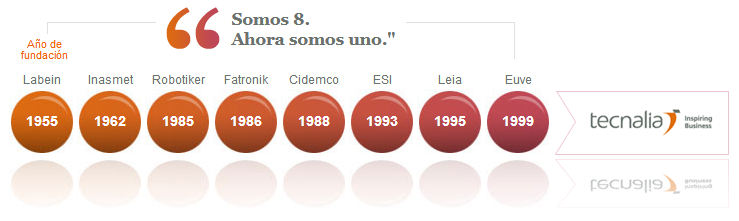
\includegraphics[scale=0.7]{Imagenes/tecnaliah}
		\caption[Empresas que conforman TECNALIA \textit{Research \& Innovation}, for L0F]{Empresas que conforman TECNALIA \textit{Research \& Innovation} \protect\footnotemark}
		\label{fig:tecnaliah}
	\end{figure}	  
\footnotetext{ https://www.tecnalia.com/es/tecnalia/historia.htm}
\par A su vez, TECNALIA junto con los centros tecnológicos, Azti y Neiker conforman a la Corporación Tecnalia, cuyo objetivo es contrubuir al desarrollo del entorno económico y social a través del uso y fomento de la innovación tecnológica, mediante el estímulo y difusión de la investigación, en un contexto internacional \footnote{http://www.tecnalia.es/}. La corporación Tecnalia nació en el año 2001, a través de la iniciativa de Inasmet, Labein y Robotiker, los cuales apostaron por unir esfuerzos e impulsar a Tecnalia de tal forma que puediera alcanzar niveles superiores de competitividad en el mercado. A raíz de esta unión otros centros tecnológicos se fueron incorporando con el pasar de los años (Figura \ref{fig:ctecnalia}), dando forma a lo que se conoce hoy como Corporación Tecnalia.\\ 
\begin{figure}[!h]
	\centering
		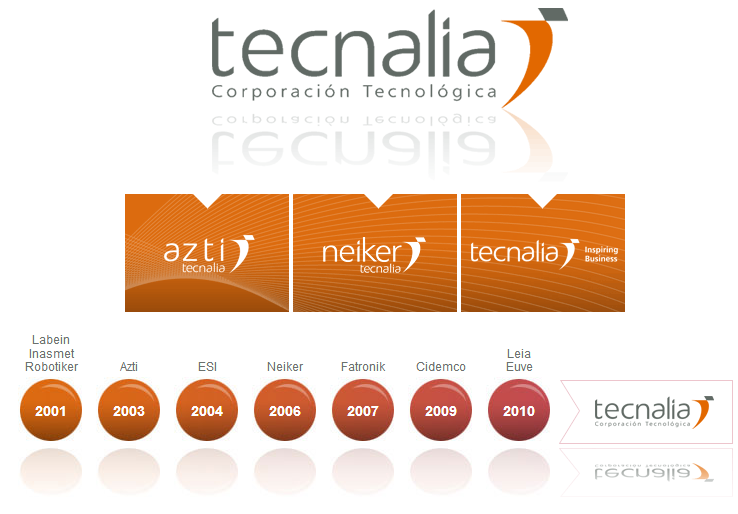
\includegraphics[scale=0.5]{Imagenes/ctecnalia}
		\caption[Empresas que conforman la Corporación Tecnalia,for L0F]{Empresas que conforman la Corporación Tecnalia \protect\footnotemark }
		\label{fig:ctecnalia}
	\end{figure}	  
\footnotetext{https://www.tecnalia.com/es/tecnalia/corporacion\-tecnalia.htm}
\section{Divisiones de TECNALIA \textit{Research \& Innovation} y Equipo de Automated Driving}
Dentro de la estructura de TECNALIA \textit{Research \& Innovation} se pueden encontrar 6 divisiones importantes:
\begin{itemize}
	\item Desarrollo sostenible.
	\item Tecnología de información y comunicación.
	\item Industria y transporte.
	\item Innovación y sociedad.
	\item Salud.
\end{itemize}
\par De estas divisiones se puede destacar la división de Industria y Transporte, la cual a su vez comprende varios focos de investigación, tales como: 
\begin{itemize}
	\item Tecnologías de fabricación  y trnasformación de materiales.
	\item Modelos predictivos de procesos de siderurgia y fundición .
	\item Tecnologías de materiales para transporte y espacio.
	\item Predicción, cotrol y mejora de características de los material.
	\item Homologación de materiales.
	\item Sistemas inteligentes de fabricación.
	\item Conducción autónoma.
\end{itemize}
\par De estos focos se resalta el de conducción autónoma, donde se desarrolló el presente trabajo. El mismo es un grupo multidisciplinario (Figura \ref{fig:equipo}) cuyo objetivo es  realizar investigaciones aplicadas a la conducción autónoma de vehículos eléctricos, esto, con el fin de poder realizar maniobras de forma segura, cómoda y eficiente en entornos urbanos e interurbanos. 
\begin{figure}[!h]
	\centering
		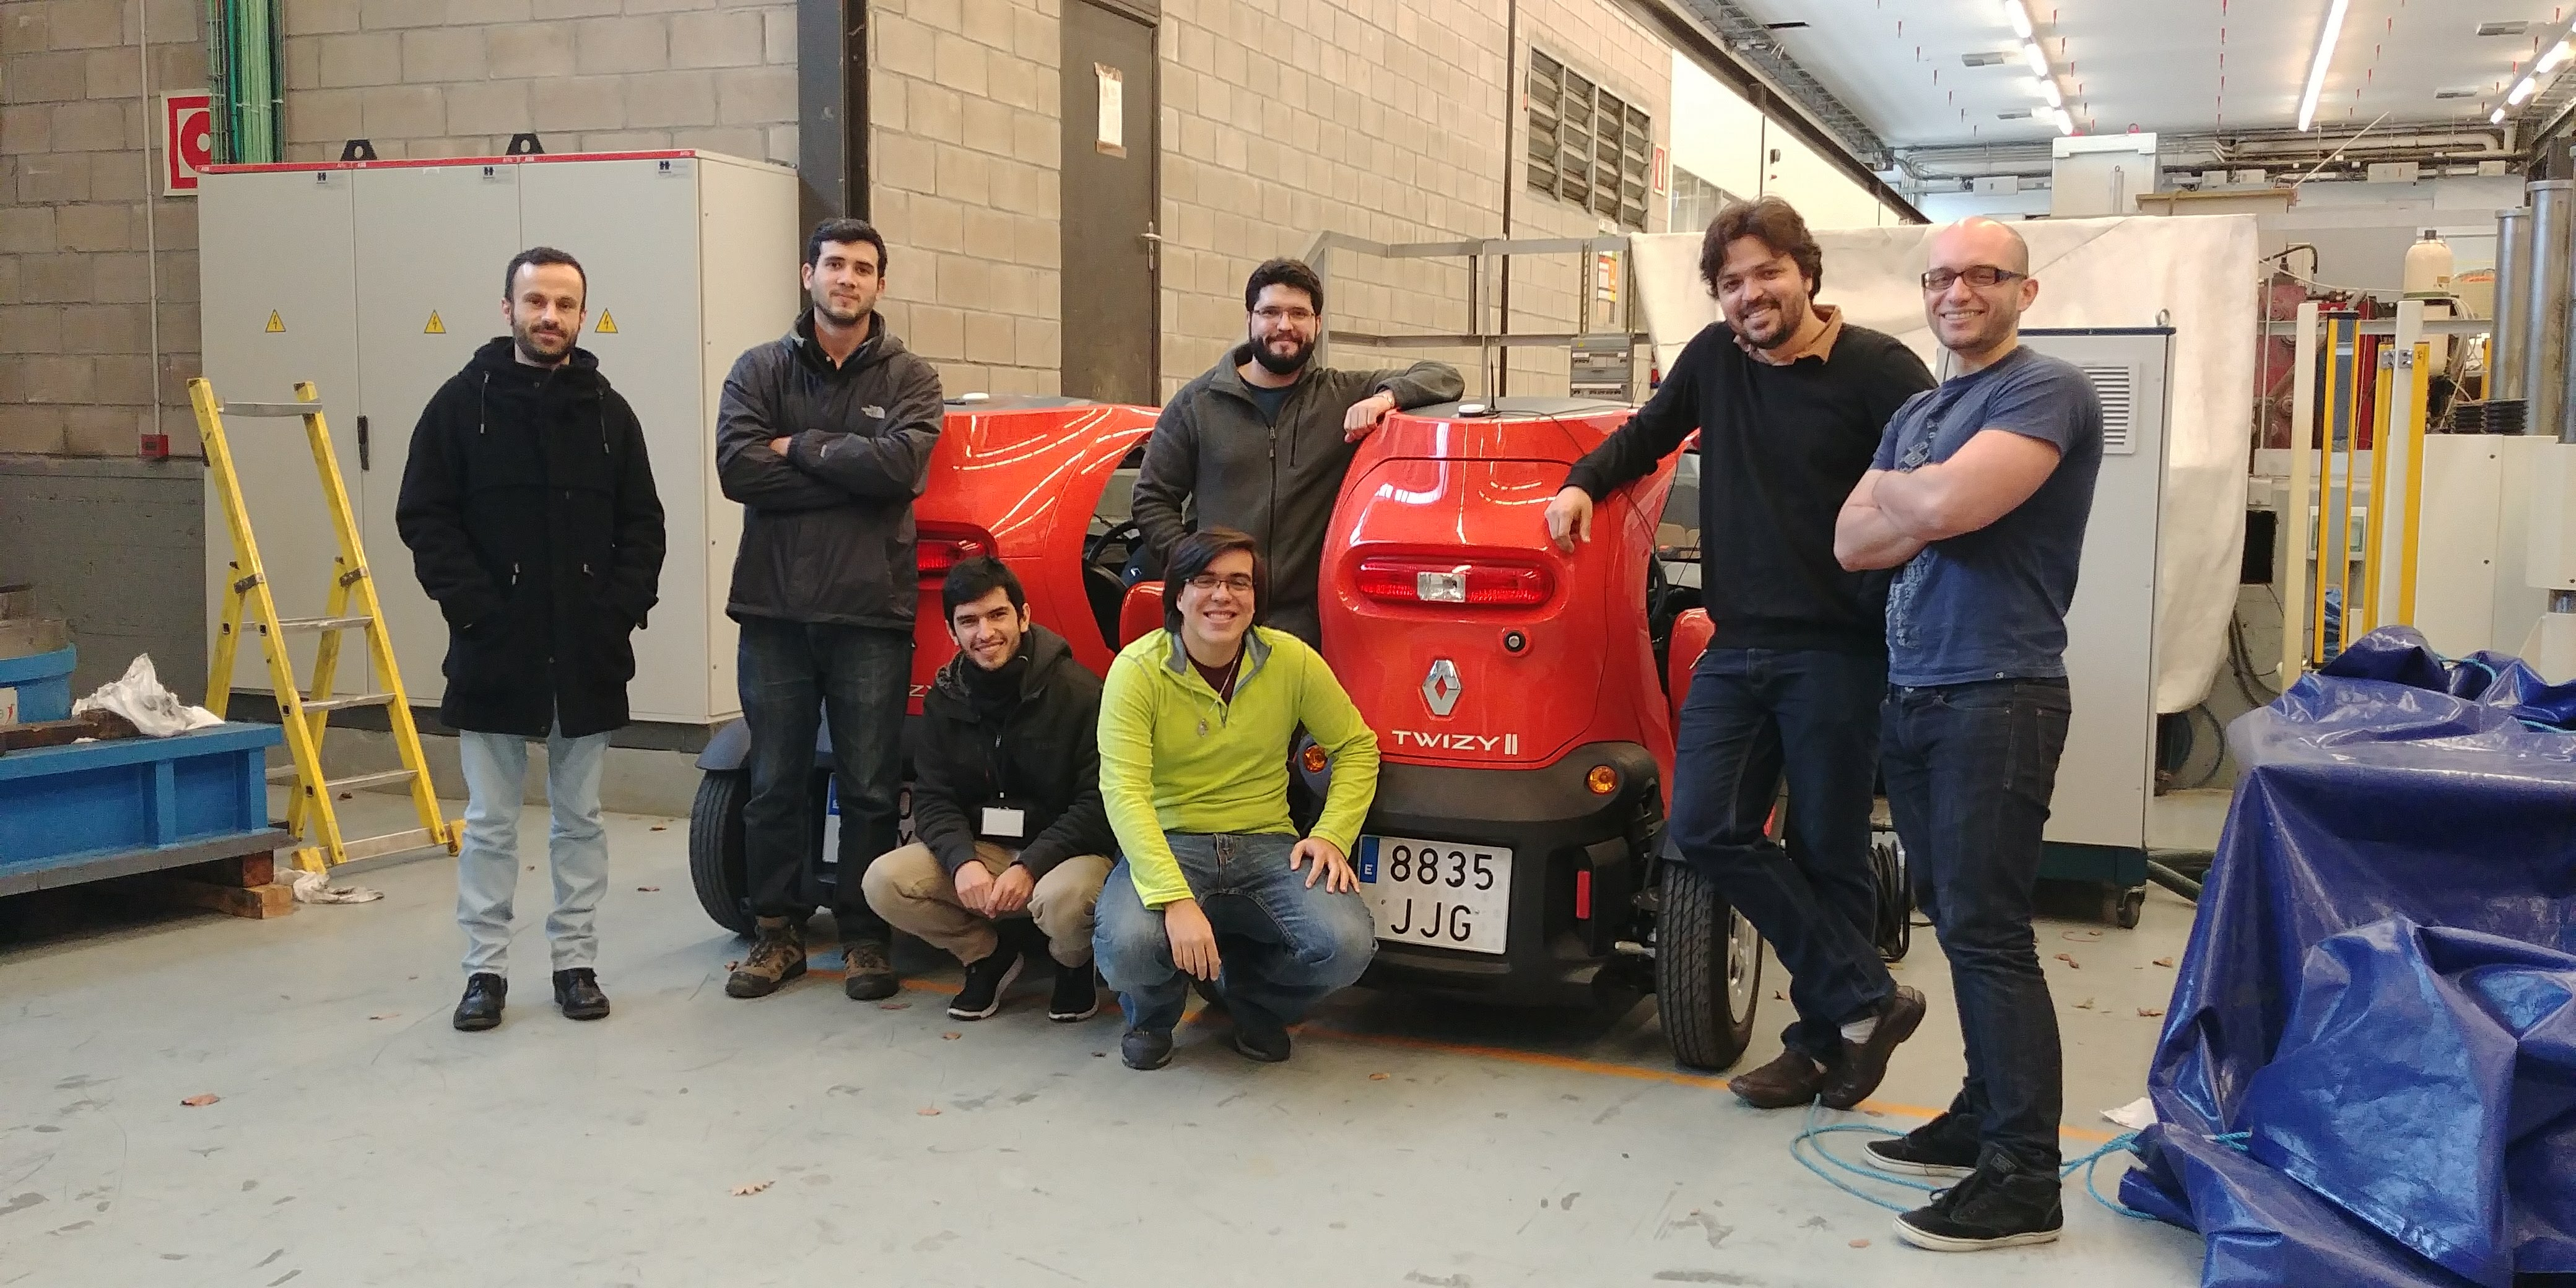
\includegraphics[scale=0.08]{Imagenes/equipo}
		\caption{Equipo de Automated Driving}
		\label{fig:equipo}
	\end{figure}	  
\subsection{Vehículos del Equipo}
Los vehículos utilizados por el equipo son dos Twizt Renault 80 (Figura \ref{fig:twizy}). Aparecieron por primera vez en el año 2009 en el salón del automóvil en Frankfurt, pero no fue si no hasta el 2011 que comenzó su producción \footnote{https://www.muyinteresante.es/innovacion/fotos/fotos-renault-twizy-coche-electrico-revolucionara-ciudades/fotos-parecido-smart\_\_\_1531}. Los Twizy disponen de un motor de 8 kW y 57 Nm, con una aceleración de 0 a 45 Km/h en 6,1 segundos, los mismos son vehículos eléctricos, que requieren una carga de 3 horas y 30 minutos, enchufados a una toma de 220 V, con 10 A\footnote{ http://www.renaulttwizy.org/renault-twizy-caracteristicas.php}.\\
\begin{figure}[!h]
	\centering
		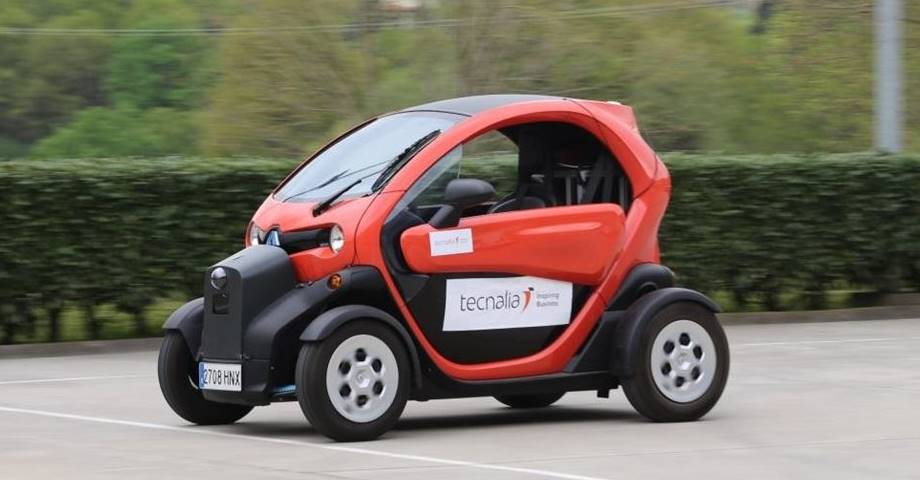
\includegraphics[scale=0.5]{Imagenes/twizy}
		\caption{Vehículo Twizy de TECNALIA}
		\label{fig:twizy}
	\end{figure}	  
\par Estos vehículos son instrumentados por la empresa española, Dirección de Tecnología Avanzada, DTA, la cual equipa los vehículos con actuadores y dispositivos electrónicos que permiten controlar los pedales y el volante del vehículo a través de Bus CAN. Esta comunicación es realizada a través de un PLC (del inglés, \textit{Programable Logic Contollers}) que sirve como interfaz entre la PC que implementa los algoritmos de conducción y los actuadores de vehículo. Cabe destacar que además de los componentes nombrados anteriormente los Twizy también fueron equipados con un GPS diferencial.\\  

\par A fines de este proyecto se resaltará el sistema de comunicación empleado en los Twizy, el cual consta de un router de la marca TP-Link conectado al CPU de cada vehículo (Figura \ref{fig:obus}), además de un dispositivo de red inalámbrico, empleado para conectar los vehículos a los routers.
\begin{figure}[!h]
	\centering
		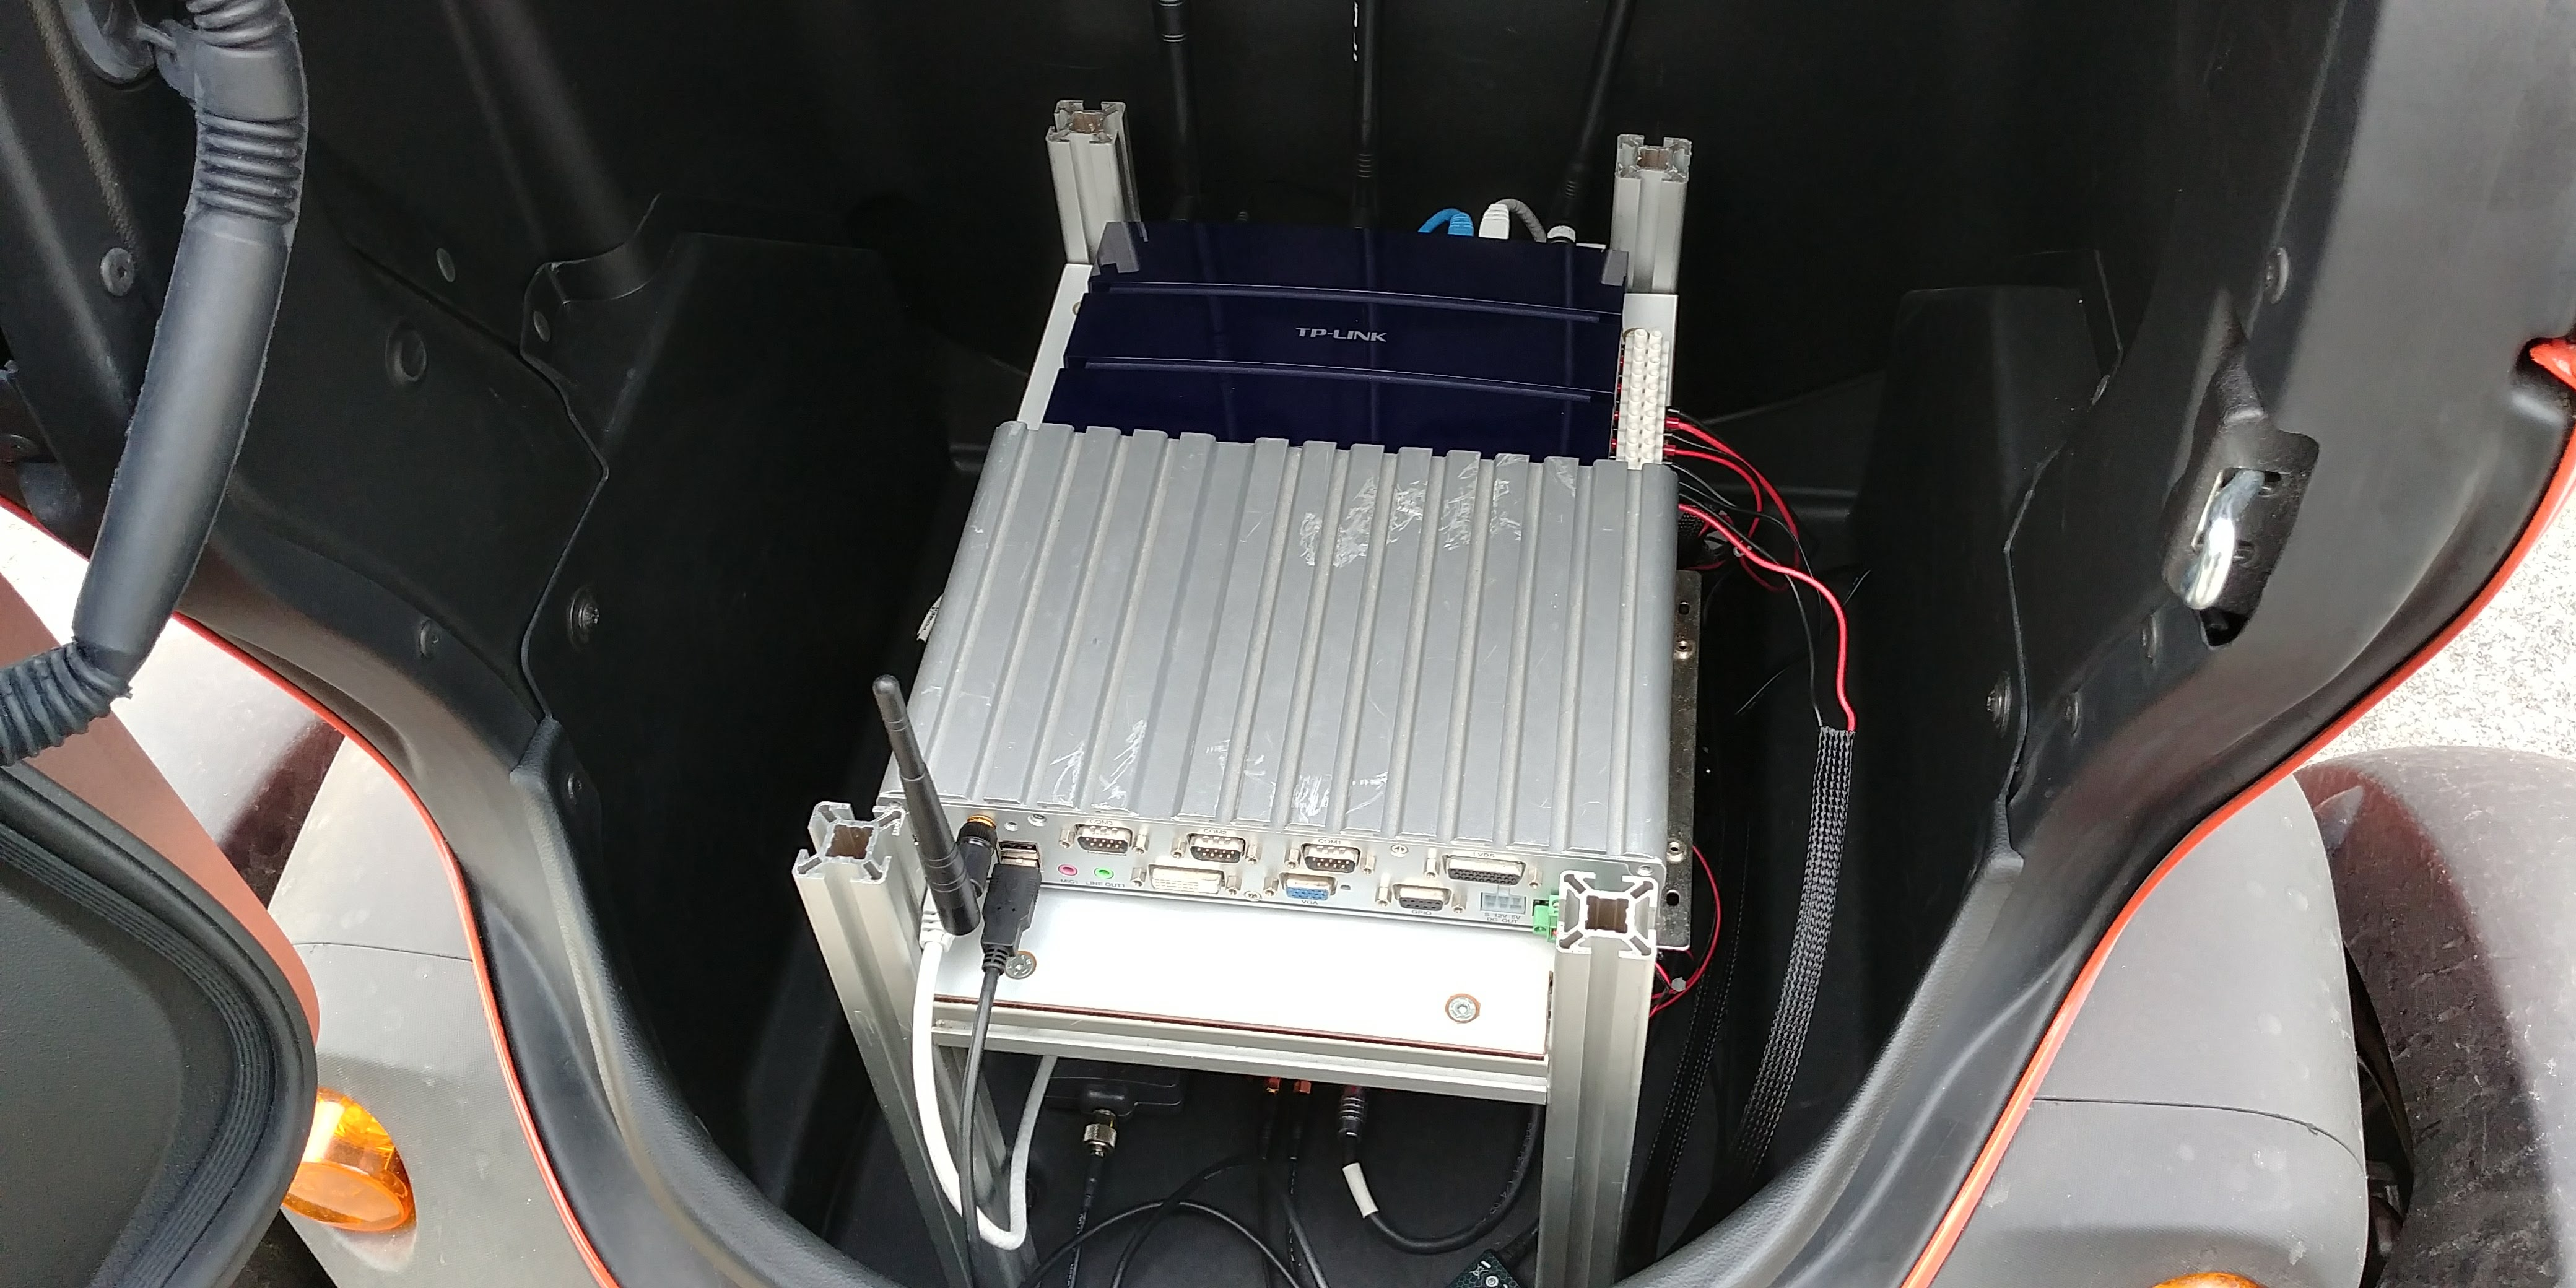
\includegraphics[scale=0.1]{Imagenes/obus}
		\caption{OBU del Twizy II}
		\label{fig:obus}
	\end{figure}	  

%%Estado del Arte: Fundamentos teóricos o Marco teorico
\chapter{Estado del Arte}\label{sec:capitulo3}
\thispagestyle{empty}
El presente capítulo establece las bases teóricas de este trabajo, de forma resumida y concisa, con el objetivo de familiarizar al lector con los conceptos necesarios para una efectiva comprensión de los temas a tratar. En este orden de ideas, se introducirán conceptos vinculados con las bases sobre las cuales estan hechas las comunicaciones hoy en día, tanto comerciales como vehículares, y de esta forma poder hablar con más criterio sobre los sistemas de comunicaciones comerciales y vehículares, describiendo los protocolos e instrumentos fundamentales para su funcionamiento.\\

\par Seguidamente, se expone la sección relacionada con los sistemas cooperativos, donde se dará a conocer toda la información de interés referente a estos sistemas, así como de los ADAS, para luego describir distintas maniobas cooperativas que se pueden realizar hoy en día. Por último se mencionará la estrategia de control implementada en la realización de las maniobras, dicha estrategia se basa en la lógica difusa, por lo que primero se procederá a definir la misma, para luego entender su utilización en el área de control.\\  
    
\section{Revisión Bibliográfica}

En esta sección se procederá a hacer un repaso a los campos de investigación relacionados a las redes de comunicación, los cuales serán de ayuda para un mejor entendimiento de los demás temas tratados en este trabajo.

\subsection{Modelo OSI}

Para efectuar una correcta comunicación entre vehículos, infraestructuras o simplemente entre dispositivos comerciales como por ejemplo unos routers, se deben tener ciertas normas que las rijan, es por esto que en esta sección se hará una breve introducción a la división de las normas de comunicación que afectan los distintos sistemas, así como la estructura lógica que deben poseer para que, sin importar las condiciones puedan interactuar entre si.\\

\par Propiamente el modelo de interconexión de sistemas abiertos, modelo OSI (del inglés, \textit{Open System Interconnection}) es una recomendación o normas de comunicaciones que deben de seguir los fabricantes para que todos los dispositivos puedan comunicarse entre ellos independientemente de la tecnología empleada \cite{anaya2016sistema}. Fue creado en el año 1980 por la organización internacional de normalización, ISO (del inglés, \textit{International Organization for Standardization}), siendo publicado oficialmente en el año 1983 por la unión internacional de telecomunicaciones, ITU (del inglés, \textit{International Telecommunications Union}).\\

\par El modelo está conformado por siete capas que definen las diferentes fases por las cuales los datos deben pasar para ir de un dispositivo a otro sobre una red de comunicaciones (ver figura \ref{fig:osi}). Sobre este esquema se han creado numerosos protocolos, los cuales cada vez están siendo más flexibles, reduciendo el número de capas y logrando transiciones de niveles no tan demarcadas, por lo que, el modelo OSI está quedando cada vez más obsoleto al pasar de los años, pero para efectos de los sistemas analizados en este trabajo la norma aún sirve como referente para su entendimiento, dicho esto se procederá a describir cada uno de los niveles.\\

\begin{figure}[hbp]
	\centering
		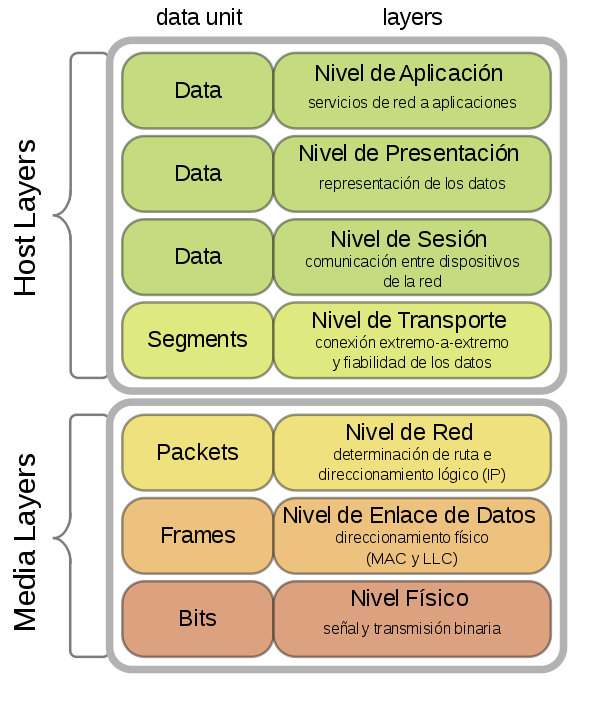
\includegraphics[scale=0.4]{Imagenes/osi}
		\caption{Torre OSI \cite{anaya2016sistema}}
		\label{fig:osi}
	\end{figure}	

\begin{itemize}
	\item Nivel físico: es el primer nivel presentado en el modelo, es el encargado de la topología de red y de las conexiones del dispositivo hacia la msima. Está más enfocado al medio físico y de como se transmite la inoformación en este.
	\item Nivel de enlace de datos: es el nivel encargado: del direccionamiento físico, del acceso al medio, de la distribución ordenada de las tramas y del control del flujo de datos.
	\item Nivel de red: se encarga de identificar el enrutamiento existente entre varias redes, es en este nivel donde se realiza el direccionamiento lógico y se establece la ruta que tienen que seguir los datos del origen hasta el receptor final.
	\item Nivel de transporte: es el encargado de realizar el transporte de los datos del dispositivo origen, al dispositivo destino, esto independientemente del tipo de red física empleada.
	\item Nivel de sesión: es el nivel encargado de mantener y controlar el enlace establecido entre los dispositivos.
	\item Nivel de presentación: en este nivel se traduce la información, de tal forma que distintos dispositivos puedan entender la información que reciben independiente de las diferentes representaciones internas que estos puedan tener.
	\item Nivel de aplicación: es el último nivel del modelo, responsable de ofrecer a las aplicaciones la posibilidad de acceder a los distintos servicios de los demás niveles, así como también definir los protocolos que utilizan estas aplicaciones para intercambiar los datos.
\end{itemize}

\subsection{Redes Ad-Hoc}
Las redes ad hoc, son redes inalámbricas que no requieren de ningún tipo de infraestructura fija ni administración centralizada, donde cada componente es una estación capaz de ofrecer servicios de encaminamiento, retransmitiendo paquetes de otras estaciones que no posean conexión inalámbrica directa. Estas redes son capaces de desplegarse tanto de forma autónoma como de forma combinada con las redes locales, y de esta manera gozar los beneficios de los servicios de internet \cite{orozco2012redes}. Vieron sus comienzos en los años 70, siendo conocidas con el nombre de radio paquetes, nombre que fue cambiado en los años 80 por el de redes ad-hoc, dicho cambio se produjo a raíz de ser implementadas en proyectos militares, los cuales las renombraron como se conoce actualmente(6). En la figura \ref{fig:adhoc} se puede encontrar un ejemplo de la distrubución del internet a través de una red ad-hoc.\\

\begin{figure}[hbp]
	\centering
		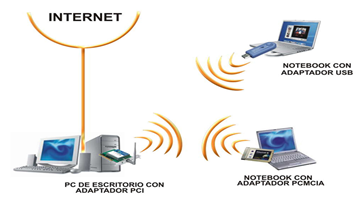
\includegraphics[scale=0.7]{Imagenes/adhoc}
		\caption[Red ad-hoc subordinada a internet]{Red ad-hoc subordinada a internet \protect\footnotemark}
		\label{fig:adhoc}
	\end{figure}	

\footnotetext{http://karolcasierra.blogspot.com/2013/04/red-ad-hoc-movil-caracteristicas-y.html}

\par Dentro de las características más resaltantes se puden encontrar:
\begin{itemize}
	\item Son nodos móviles, es decir los dispositivos de las redes ad-hoc pueden cambiar de posición a placer.
	\item Constan de una topología variable, ya que los dispositivos se pueden mover y formar nuevos elances con otros dispositivos, siempre y cuando pertenezcan a su área de cobertura.
	\item Tienden a realizar cambios de ruta, esto debido a su topología variable, lo cual produce que la ruptura de enlaces sea un problema frecuente, lo que origina que se varien las rutas constantemente.
	\item Poseen autonomía limitada causada por la portabilidad de los dispositivos, ya que estos vienen limitados en cuanto a la duración de la batería.
	\item Tienen limitaciones en los enlaces inalámbricos, ya que estos enlaces se caracterizan por tener un ancho de banda reducido, asi como, una disposición a comerter errores, defectos que se ven compensados por la cualidad de repetidor de nodos. 
	\item Gozan de la ausencia de infraestructura, esto debido a que no existe ningún tipo de entidad centralizada que rijan las conexiones, por lo cual los dispositivos pueden desempeñar los papeles de host o router en cualquier momento.
\end{itemize}

 Según su aplicación se pueden clasificar de la siguiente manera: 
\begin{itemize}
	\item Redes ad-hoc móviles, MANET's (del inglés, \textit{Moblie Ad-Hoc Networks}).
	\item Redes inalámbricas malladas.
	\item Redes de sensores.
	\item Redes ad-hoc vehiculares, VANET's (del inglés, \textit{Vehicular Ad-Hoc Networks}).
\end{itemize}

\subsection{Protocolos de Transporte}

Entre las capas expuestas anteriormete se encuentra la de transporte, pieza fundamental de la arquitectura del modelo. Desempeñando un papel crítico al proporcionar servicios de comunicación a los procesos de aplicación que se ejecutan en hosts diferentes. Dentro de estos protocolos se pueden destacar tres, dos para las comunicaciones entre componentes comerciales, e internet, UDP y TCP, y uno para las comunicaciones vehiculares, \textit{Geonetwork}.

\subsubsection{UDP}

El protocolo de datagrama de usuario, UDP (del inglés, \textit{User Datagram Protocol}) es un protocolo del nivel de transporte basado en el intercambio de datagramas El mismo permite el envío de dichos datagramas a través de la red sin que se haya establecido una conexión previa, esto debido a que los mismos incorporan sufiente información de direccionamiento. Además no posee confirmación ni control de flujo, lo que origina que los paquetes puedan adelantarse unos a otros y se pierdan en el camino. Este tipo de protocolo es mayormente empleado para servidores DHCP, BOOT y DNS, y demás servicios en los que el intercambio de paquetes de la conexión son mayores, o  no son rentables con respecto a la información trnasmitida (3). Entre las principales características se encuentra que:\\

 \begin{itemize}
	\item Es un protocolo mínimo de nivel de transporte orientado a los mensajes.
	\item Proporciona una sencilla interfaz entre la capa de red y la capa de aplicación.
	\item No otorga garantías para la entrega de sus mensajes.
	\item Es empleado cuando resulta más importante transmitir con velocidad que garantizar el hecho de que los mensajes lleguen completos, como es el caso de la transmisión de audio y video.
\end{itemize}

\subsubsection{TCP}
El protocolo de control de transmisión, TCP (del inglés, \textit{Transmission Control Protocol}) es un protocolo orientado para crear conexiones entre computadoras de una misma red. En este caso el protocolo garantiza que los datos serán entregados a su destino sin errores y en el mismo orden en el cual fueron transmitidos. TCP da soporte a muchas aplicaciones relacionadas al internet, como lo pueden ser: navegadores, intercambio de ficheros, proramas de mensajería entre otros (3). Entre las principales características se ecnuentra que: 

\begin{itemize}
	\item Es orientado a la conexión, es decir las computadoras se conectan para intercambiar datos, sincronizandose para manejar el flujo de paquetes y adaptarse a la congestión de red.
	\item Emplea la técnica cheksum, con la cual verifica que los paquetes no esten corruptos.
	\item El receptor regresa un acuse de recibo al transmisor indicando que ya llegaron los paquetes.
	\item En caso de se desborde el buffer receptor, el mismo descarta los paquetes, ocasionando que el transmisor reduzca la tasa de envío.
	\item En caso de que el mensaje no se reciva de forma adecuada e receptor puede pedir la retransmisión del mismo.
\end{itemize}

\section{Sistemas de Comunicación}

A continuación se presentan los fundamentos sobre los sistemas de comunicación analizados en este trabajo.\\ 

\subsection{Sistemas de Comunicación Comerciales}
Los sistemas de comunicación comerciales son aquellos elementos empleados para conectar distintos dispositivos, ya sean computadoras, celulares, televisores, etc. Son nombrado como comerciales, ya que son de acceso al público sin ninguna restricción. Estos sistemas hacen uso de los dispositivos de comunicación como lo son los routers, o enrutadores y los puntos de acceso, AP (del inglés, \textit{Access Point}) \cite{pellejero2006fundamentos}.\\

 \begin{itemize}
	\item Router: es un dispositivo que porporciona conectividad a nivel de red, o nivel tres del modelo OSI, cuyo principal objetivo consiste en enviar o encaminar paquetes de datos de una red a otra, es decir interconectar subredes (Figura \ref{fig:router}).

\begin{figure}[!h]
	\centering
		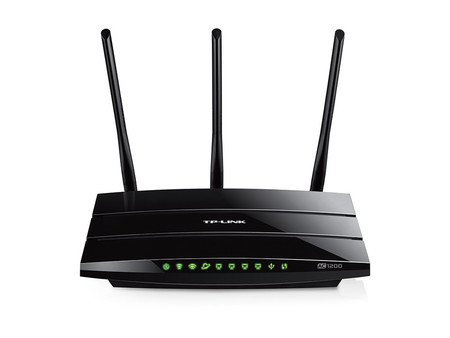
\includegraphics[scale=0.5]{Imagenes/router}
		\caption{Ejemplo de un router}
		\label{fig:router}
	\end{figure}	

	\item Punto de Acceso: es un dispositivo de red que interconecta equipos de comunicaciones inalámbricos, para formar una red, en la cual se conectan distintos elementos móviles o trajetas de red inalámbricas (Figura \ref{fig:pa}).

\begin{figure}[!h]
	\centering
		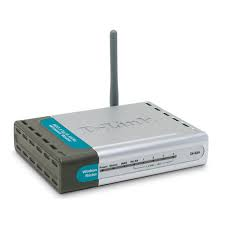
\includegraphics[scale=0.5]{Imagenes/pa}
		\caption{Ejemplo de un punto de acceso}
		\label{fig:pa}
	\end{figure}	
\end{itemize}   

\subsubsection{W-Lan}

Las redes WLAN (Figura \ref{fig:wlan}). se pueden definir como un sistema de comunicación que transmite y recibe datos utilizando ondas electromagnéticas, en vez de un cable trenzado o fibra óptica utilizado en las LAN, y que proporciona conectividad inlámbrica, dentro de un área de cobertura determinado, entre 10 m y 100 m\cite{varela2002redes}. Dentro de sus características más importantes se encuentran:\\

\begin{figure}[!h]
	\centering
		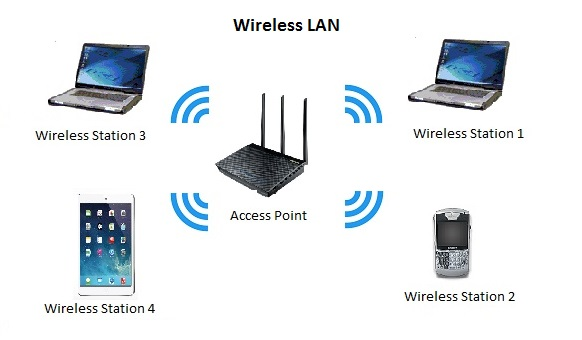
\includegraphics[scale=0.6]{Imagenes/wlan}
		\caption[Ejemplo de una WLAN, for L0F]{Ejemplo de una WLAN \protect\footnotemark}
		\label{fig:wlan}
	\end{figure}	
\footnotetext{http://tiposderedesgeograficamente.blogspot.com/}

\begin{itemize}
	\item Movilidad: permite transmitir información en tiempo real en cualquier lugar de la organización o empresa a cualquier usuario.
	\item Facilidad de instalación: al no usar cables, se evitan arduos trabajos de instalación de los mismos, por lo que se reduce el tiempo neceseario para poder emplear los servicios de red, además de proporcionar los servicios a múltiples usuarios de forma instantánea.
	\item Flexibilidad: puede llegar a donde no puede el cable, aumentando así el rango de cobertura. Además de ser más económica que los sistemas cableados.
\end{itemize}

Las WLAN poseen un gran número de escenarios en los cuales pueden ser empleados, siendo los mas destacados destacados:\\

\begin{itemize}
	\item Escenario residencial: una línea telefónica terminada en un router ADSL al cual se conecta un punto de acceso, para formar una red WLAN que de cobertura a varios dispositivos.
	\item Redes corporativas: una serie de puntos de accesos distruibuidos en varias áreas de la empresa que conforman redes autonómas.
	\item Acceso a internet desde distintos lugares: desde cafeterías hasta medios de transportes que poseen conexión via satelital, los cuales pueden proporcionar servicios de internet a los usarios conectados a su red.
	\item Usos corporativos e industriales: como interconexiones de máquinas y distintos dispositivos.   
\end{itemize}

\par Otro uso que, tomando en cuenta sus específicas condiciones no es tán común, como pueden ser cualquiera de los mencionados, es el uso en comunicaciones vehiculares, esto debido a que son conexiones con características muy particulares que una simple red WLAN no puede garantizar cumplir, a excepción de algunos casos, donde bajo ciertas condiciones se puede recrear este tipo de comunciaciones, como se va a mostrar más adelante en los siguientes capítulos.\\    

\par Las WLAN emplean principalmente las bandas industriales, científicas y médicas, ISM (del inglés, \textit{Industrial, Scientific and Medical}), que comprenden las frecuencias entre 902-928 MHz, 2.4-2.4835 GHz y 5.725-5.850 GHz. Estas bandas son de uso común y no requieren de licencia para utilizarlas. Debido a que estas frecuencias no requieren de licencia para operar las WLAN poseen un gran potencial de mercado logrando así competir con otros tipos de tecnologías de acceso, lo cual obliga que se desarrolle un marco regulatorio que permita el uso eficiente y compartido de las mismas. En este ámbito es donde entra el instituto de ingenieros eléctricos y electrónicos, IEEE (del inglés, \textit{Institute of Electical and Electronic Engineers}), el cual dasarrolló los estándares que rigen este tipo de red, estándares que se procederán a describir a continuación.

\subsubsection{IEE 802.11}  

Las redes WLAN cumplen con los estándares genéricos aplicables al mundo de las LAN cableadas, pero necesitan una normativa adicional que defina el uso y acceso de los recursos radioeléctricos. Estas normativas definen de forma detallada los protocolos para las capas física, de control de acceso al medio, MAC (del inglés, \textit{Media Acces Control}) y de control de enlace de datos, DLC (del inglés, \textit{Data Link Level}) que regulan la conexión vía radio\cite{camargo2009modelo}. El primer estándar donde se especificaron estas capas fue el IEEE 802.11 en el año 1997.\\

\par Este estándar especifica una frecuencia de operación de 2.4 GHz con velocidades de transmisión de 1 y 2 Mbps. Desde esta versón inicial el IEEE 802.11 WG (del inglés, \textit{Working Group}) ha llevado a cabo diferentes revisiones a través de varios grupos de trabajo especializados en distintas áreas.\\

 \par Antes de repasar cada uno de estos estándares se procederá a describir el esquema de las capas (Figura \ref{fig:ieee}), que es común para cada uno ellos.\\ 

\begin{figure}[H]
	\centering
		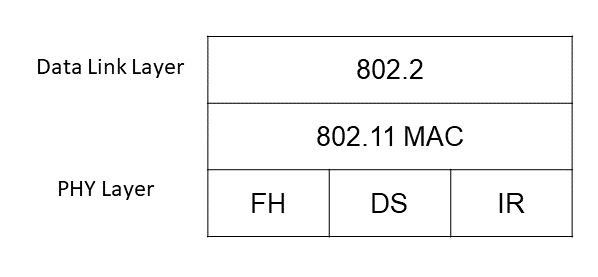
\includegraphics[scale=0.5]{Imagenes/ieee}
		\caption{Capas del IEEE 802.11 \cite{{pellejero2006fundamentos}}}
		\label{fig:ieee}
	\end{figure}	

\par Donde:

 \begin{itemize}
	\item La Capa física: define la modulación y la señalización característica de la transmisión de datos. Como se mencionó anteriormente estas redes operan en la banda de 2.4 GHz a excepción del IEEE 802.11 a que opera en la banda de 5 GHz, ocupando aproximadamente 83 MHz de ancho de banda. Para la transmisión y recepción de tramas se tienen tres opciones:
	\begin{itemize}
		\item Espectro expandido por secuencia diercta, DSS (del inglés, \textit{Direct Sequence Spread Spectrum})
		\item Espectro expandido por salto de frecuencia, FHSS (del inglés, \textit{ Frequency Hopping Spread Spectrum})
		\item Modulación por división ortogonal de frecuencias, OFDM (del inglés, \textit{Orthogonal Frequency Division 					Multiplexing})
	\end{itemize}	
	\item Capa MAC: es la capa de control del medio, para la cual se diseñó un mecanismo que puede reaccionar positivamente ante 		perturbaciones ambientales, variaciones en la potencia de la señal, y las repentinas conexiones y desconexioes en la red. Este 		mecanismo es conocido como, acceso múltiple por detección de portadora y prevención de colisiones, CSMA/CA (del inglés, \textit{Carrier Sense Multiple Acces with Collision Avoidance}), que funciona de la siguiente forma, si la estación que desea 			transmitir escucha el medio de transmisión, pero si el medio esta ocupado significa que otra estación está transmitiendo y por lo 		tanto debe de retrasar su transmisión hasta que se libere.
\end{itemize}

\par Ya conociendo la estructura básica de del IEEE 802.11 ahora se procede a hablar sobre cada uno de los estándares \cite{pellejero2006fundamentos}.

 \begin{itemize}
\item 802.11a: es un estándar también conocido como Wi-Fi5. Su misión es crear un estándar de WLAN en la banda de 5 GHz, capaz de alcanzar tasas de hasta 54 Mbps. Se publicó en el 1999.
\item  802.11b: es un estándar también conocido como Wi-Fi. Está pensado para WLAN en la banda de 2.4 GHz, con una tasa que alcanza los 11 Mbps. Fue publicada en el 1999.
\item  802.11c: provee de documentación a la 802.11 sobre procedimientos específicos MAC de la Organización Internacional para la Comisión Electrónica de Estandarización Internacional (ISO/IEC). Su trabajo está concluido.
\item  802.11d: su misión es definir nuevos requerimientos para la capa física para hacer funcionar la 802.11 en otros países donde no es posible implementar 802.11, por no tener la banda de 2.4 GHz libre o ser más corta.
\item  802.11e: este grupo trabaja en los aspectos relacionados con la calidad de servicio, QoS (del inglés, \textit{Quality of Service}). En el mundo de las redes de datos, calidad de servicio significa poder dar más prioridad de transmisión a unos paquetes de datos que a otros, dependiendo de la naturaleza de la información (voz, vídeo, imágenes, etc.).
\item  802.11f: básicamente, es una especificación que funciona bajo el estándar 802.11g y que se aplica a la intercomunicación entre puntos de acceso de distintos fabricantes, permitiendo el roaming o itinerancia de clientes.
\item  802.11g: pretende desarrollar una extensión de la 802.11b, \textit{higherspeed PHY}, capaz de mantener la compatibilidad con la 802.11b. El objetivo inicial de este era alcanzar al menos 20 Mbps y se ha conseguido llegar hasta los 54 Mbps.
\item  802.11h: una evolución del IEEE 802.11a que permite asignación dinámica de canales y control automático de potencia para minimizar los efectos de posibles interferencias. Este punto es una de las desventajas que tiene IEEE 802.11a frente a su competidor europeo HiperLAN/2 (que también opera en la banda de los 5 GHz).
\item 802.11i: este estándar permite incorporar mecanismos de seguridad para redes inalámbricas, ofrece una solución interoperable y un patrón robusto para asegurar datos. Mejora los mecanismos de autenticación y seguridad de la 802.11, como es WEP. El sistema sobre el que se está trabajando se conoce como TKIP (del inglés, \textit{Temporal Key Integrity Protocol}).
\item 802.1x: pretende mejorar los mecanismos de seguridad de la 802.11, con los protocolos de seguridad extendida, EAP (del inglés, \textit{Extensible Authentiticatiion Protocol}).
\end{itemize}

\subsection{Sistemas de Comunicación Vehicular}

Los sistemas de comunicación vehicular son los sistemas empleados para la conexión entre vehículos, infraestructuras y peatones, están compuestos básicamente de dos componentes, las unidades a bordo, OBU's (del inglés, \textit{On Board Untis}) y las unidades en vía, RSU's (del inglés, \textit{ Road Side Unit's}) (Figura \ref{fig:obursu}), las cuales tienen como finalidad dar soporte a las comunicaciones de las aplicaciones de diversas naturalezas. La principal diferencia entre ambas, es el propósito por el cual fueron diseñadas. Las OBU's están destinadas a los vehículos, por lo cual pueden cambiar su posición, mientras que las RSU's se encuentran en las infraestructuras, lo que implica que son estáticas.\\

\begin{figure}[!h]
	\centering
		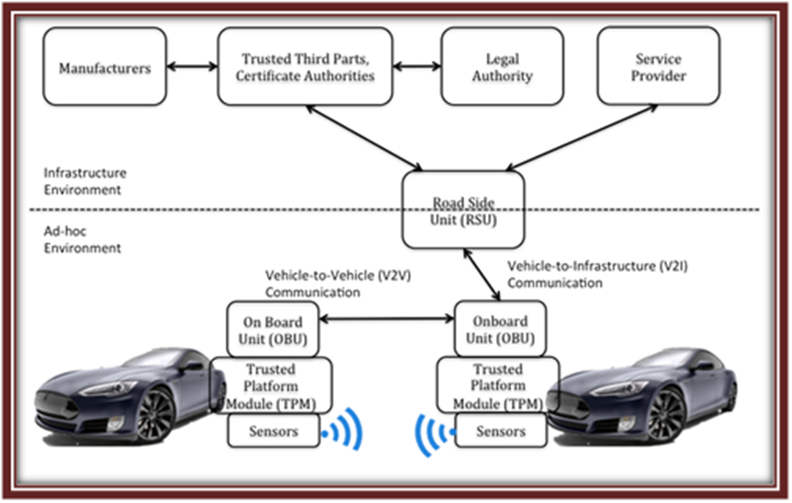
\includegraphics[scale=0.8]{Imagenes/obursu}
		\caption[Ejemplo de la comunicación entre las OBU's y las RSU's, for L0F]{Ejemplo de la comunicación entre las OBU's y las RSU's \protect\footnotemark}
		\label{fig:obursu}
	\end{figure}	
\footnotetext{https://www.cse.wustl.edu/\~jain/cse571-14/ftp/vanet\_security/index.html}

 \par El objetivo de estos sistemas es comunicar los distintos componentes que conforman los ITS, es por eso que se clasifican en cinco tipos\cite{da2014data} (Figura \ref{fig:v2x}):

\begin{itemize}
	\item Vehículo con vehículo, V2V (del inglés, \textit{Vehícle to Vehícle}): es el tipo de comunicación entre vehículos, la cual no necesita de una infraestructura fija que maneje la interacción entre los mismos, es usada por lo general en aplicaciones de seguridad, prevención de riesgos y para esparcir información. Debido a su natruraleza móvil este es un tipo de red ad-hoc vehícular, mejor conocida como VANET's.
	\item Vehículo con infraestructura, V2I (del inglés, \textit{Vehicle to Infrastructure}): es el tipo de comunicación entre vehículos e infraestructura, es usada para esparcir información, así como para recolección de data.
	\item Vehículo con peatón, V2P (del inglés, \textit{Vehicle to Pedestrian}): es el tipo de comunicación entre vehículos y peatones, que en este caso engloba tanto personas que se movilizan a pie, como en bicicleta. En general se utiliza en aplicaciones de prevención de riesgo, así como para la obtención de los servicios de internet por parte de los peatones.
	\item Arquitectura híbrida, V2X (del inglés, \textit{Vehicle to Everething}): es la combinación entre los escenarios planteados anteriormente, V2V, V2I, V2N y V2P. En este caso los vehículos intercambian información con las infrastructuras de forma multi salto o de un solo salto, dependiendo de las distancias.
	\item Vehículo con la red, V2N (del inglés, \textit{Vehicle to Network}): es el tipo de conexión entre los automóviles y los servidores de aplicaciones, el cual tiene como principal función dotar a los carros con los servicios de internet.
\end{itemize}

\begin{figure}[!h]
	\centering
		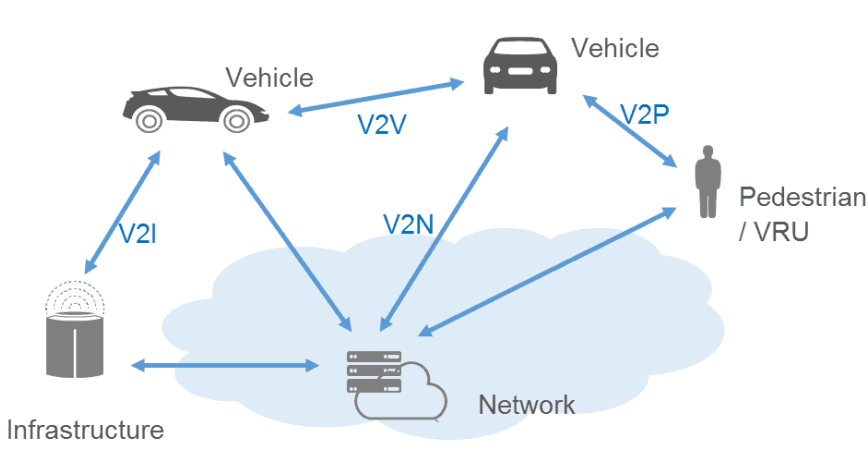
\includegraphics[scale=0.4]{Imagenes/v2x}
		\caption[Tipos de comunicaciones vehículares, for L0F]{Tipos de comunicaciones vehículares \protect\footnotemark}
		\label{fig:v2x}
	\end{figure}	
\footnotetext{http://www.traffictechnologytoday.com/news.php?NewsID=82371}

\subsubsection{Vanets}
El uso de las diversas tecnologías inalámbricas enfocadas a vehículos ha sido objeto de estudio desde los años 70, teniendo como uno de los proyectos pioneros el desarrollado por el ministerio de industria y comercio internacional de Japón, MITTI (del inglés, \textit{Ministry of International Trade and Industry}), que consistió en un sistema integral automovilístico de control de tráfico, CACS (del inglés, \textit{Comprehensive Automovile Traffic Control System}), cuyo objetivo fue reducir la congestión vehicular y disminuir el número de accidentes de tráfico, aportando a los conductores información sobre las vías y asistencia en caso de emergencias \cite{orozco2012redes}.\\

\par En 1986, el proyecto PROMETHEUS (del inglés, \textit{PROgraMme for Euripean Traffic withc Highest Efficiency and Unprecedented Safety}) conformada por 19 países de Europa, impulsó la investigación en comunicaciones móviles inalámbricas con la propuesta Prometheus SR-MRN (del inglés, \textit{Short-Range Mobile Radio Network}), y de esta forma sentó un precedente en el desarrollo de sistemas de conducción vehicular automatizados \cite{heistert}.\\

\par En la década de los 90 \cite{zeadally2012vehicular} surgieron varios proyectos como, PATH (del inglés, \textit{California Partners for Advanced Traffic and Higways}), ASV (del inglés, \textit{Advanced Safety Vehicle}) y PROMOTE CHAUFFEUR, que desarrollaron distintas áreas de la comunicación vehicular, tales como: estándares, arquitectura y diseño de la red, protocolos de enrutamiento, creación de aplicaciones y mejora en los aspectos de seguridad. Dichos progresos conllevaron que el concepto de VANET tomara relevancia en la comunidad científica,  produciendo de esta forma que se realizaran cada vez más proyectos buscando la optimización de este tipo de red. En la figura \ref{fig:vaneth} se pueden encontrar los distintos proyectos realizados desde su comienzos hasta el año 2010.\\

\begin{figure}[!h]
	\centering
		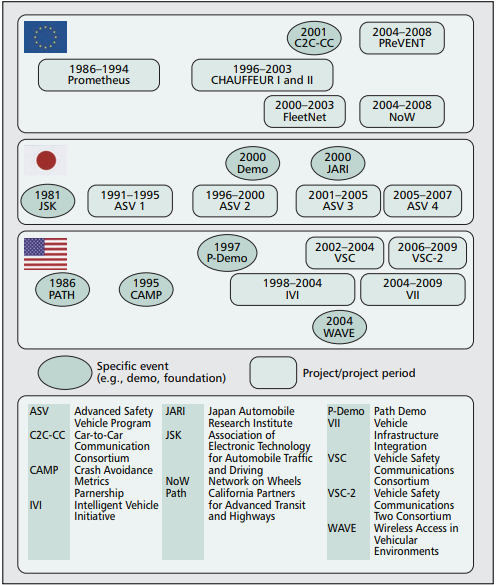
\includegraphics[scale=0.9]{Imagenes/vaneth1}
		\caption{Proyectos relacionados a las VANETS a lo largo de la historia \cite{hartenstein2008tutorial}}
		\label{fig:vaneth}
	\end{figure}	

\par De esta forma se puede decir que las VANET's son una derivación de las redes ad-hoc, donde cada vehículo se define como un nodo de la red capaz de intercambiar información con otros vehículos o con puntos de acceso estacionarios ubicados en las vías.\\

\par Al ser un derivado de las redes ad-hoc, las VANET's poseen las mismas características que estas, con la diferencia, que en este caso los nodos al ser vehículos varian su posición de forma más rápida, lo que produce desconexiones más frecuentes, ocasionando que el intercambio de datos se tenga que realizar de forma muy rápida, y sea propenso a sufrir interferencias de otros enlaces. Debido a estos inconveninetes este tipo de red se diseñó con la intención de que los mismos se afectaran lo menos posbile, así pues distintos entes realizaron sus propias especificaciones, pudiéndose resaltar tres: el ETSI, en Europa, la Comisión Federal de Comunicaciones de Estados Unidos, FCC (del inglés, \textit{Federal Communications Commision}) y la Asociación de Industrias y Negocios de Radio, ARIB, (del inglés, \textit{Association of Radio Industries and Businesses}) \cite{zeadally2012vehicular}. Estas especificaciones se pueden encontrar en la tabla \ref{tab:vanl}.\\

% Table generated by Excel2LaTeX from sheet 'Hoja1'
\begin{table}[htbp]
  \centering
\resizebox{\textwidth}{!}{
    \begin{tabular}{|c|p{14.07em}|p{16em}|c|}
    \toprule
    Característica & \multicolumn{1}{c|}{Japón} & \multicolumn{1}{c|}{Europa} & USA \\
    \midrule
    Tipo de comunicación & Half-duplex (OBU)/Full-duplex(RSU) \& Half-duplex & \multicolumn{1}{c|}{Half-duplex} & Half-duplex \\
    \midrule
    \multicolumn{1}{|p{8.715em}|}{Banda y radiofrecuencia} & Ubicado en la banda de 5.8 GHz, con un ancho de banda de 80 MHz \& Ubicado en la banda de 5.9 GHz & Ubicado en la banda de 5.9 GHz, con un ancho de banda de 20 MHz & \multicolumn{1}{p{12.57em}|}{Ubicado en la banda de 5.9 GHz,con un ancho de banda de 75 MHz} \\
    \midrule
    Canales & \multicolumn{1}{c|}{30 metros} & \multicolumn{1}{c|}{De 15 a 20 metros} & 1000 metros \\
    \midrule
    Tipo de modulación & 2-ASK, 4-PSK (ASK: modulación por desplazamiento de amplitud, del inglés, \textit{Amplitud-Shift Keying}, PSK: modulación por desplazamiento de fase, del inglés, \textit{Phase Shift Keying}) & OFDM & OFDM \\
    \bottomrule
    \end{tabular}}%
\caption{Comparativa de las especificaciones de las VANET's}
  \label{tab:vanl}%
\end{table}%

\par Para este trabajo las normas a considerar son las realizadas en Europa, ya que, el proyecto fue realizado en España, país que se rije bajo esta normativa.       

\subsubsection{DSRC}

Las comunicaciones de corto alcance, DSRC (del inglés, \textit{ Dedicated Short Range Communication}) son comunicaciones inalámbricas bidireccionales, de medio a corto alcance, que permiten una transmición de data a alta velocidad, lo cual es una cualidad muy importante a la de hora enviar los mensajes de seguridad y de las aplicaciones preventivas. Debido a su estructuración, la misma está diseñada específicamente para el uso en comunicaciones V2V y V2I. En Europa las DSRC están diseñadas bajo la arquitectura de acceso a comunicaciones terrestres móviles, CALM (del inglés, \textit{Communications Acces for Land Mobiles}) (Figura \ref{fig:calm}), las cuales están basadas en el modelo de capas OSI.\\

\begin{figure}[!h]
	\centering
		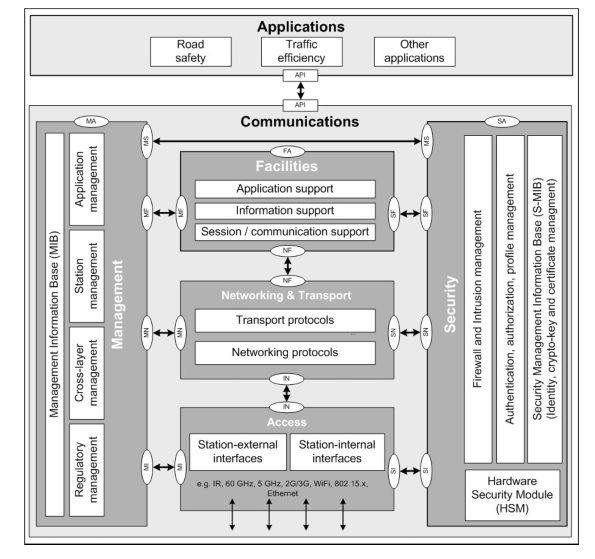
\includegraphics[scale=0.9]{Imagenes/calm}
		\caption{Arquitectura CALM \cite{anaya2016sistema}}
		\label{fig:calm}
	\end{figure}	

\par Esta arquitectura además de ser diseñada por el ETSI, también fue creada por varios entes europeos como lo son: la organización europea de estandarización, ESO's (del inglés, \textit{European Standardization Organizations}) y el comité europeo de estandarización, CEN (del inglés, \textit{European Committee for Standardization}). Unidos, realizaron la ISO/TC204WG16, que es un conjunto de documentos donde se detalla toda la información referente a las DSRC. En la Figura \ref{fig:layers} se puede observar una distribución de la arquitectura CALM, un poco más detallada, indicando las capas con sus respectivos contenidos y los documentos donde se hablan de las mismas \cite{festag2014cooperative}.\\

\begin{figure}[!h]
	\centering
		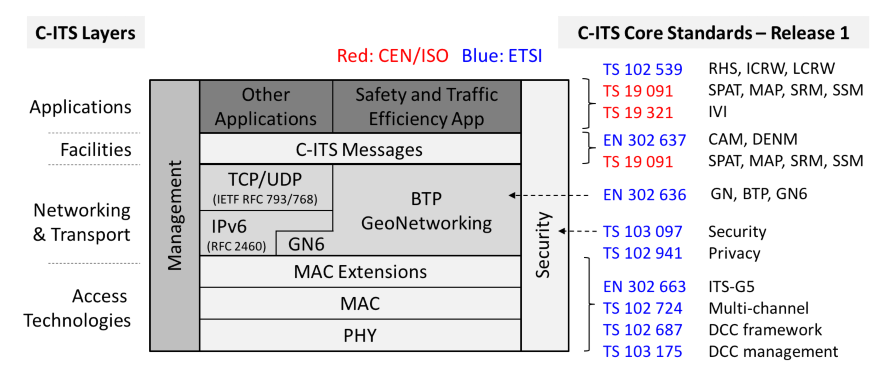
\includegraphics[scale=0.7]{Imagenes/layers}
		\caption{Capas de la arquitectura CALM, con los respectivos documentos donde se encuentran \cite{festag2014cooperative}}
		\label{fig:layers}
	\end{figure}	

\par Entonces, cada capa posee las siguientes especificaciones:

\begin{itemize}
	\item Capa de acceso: está basada en el estándar IEEE 802.11p, donde se poseen tres bandas de frecuencia de 5 GHz, distruibuidas como se muestra en la Figura \ref{fig:fisi}, donde los dos primeros canales se emplean para aplicaciones cualquieras, dejando los otros 5 para ellas aplicaciones de segurdad. Dichos canales de poseen un ancho de 20 MHz, mientras que los demás de 10 MHz. En esta capa se tienen dos niveles: el nivel físico y de MAC, siendo los equivalentes a los niveles 1 y 2 del modelo OSI.\\

\begin{figure}[!h]
	\centering
		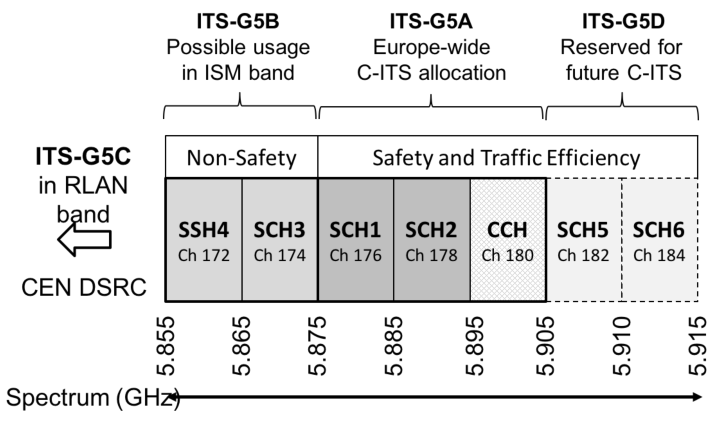
\includegraphics[scale=0.7]{Imagenes/fisi}
		\caption{Distribución de canales en la capa de acceso \cite{festag2014cooperative}}
		\label{fig:fisi}
	\end{figure}	

	\subitem Nivel físico: es en donde se da la transmisión física, la cual emplea, al igual que el estándar IEEE 802.11a una OFDM con 52 subportadoras, de las cuales 48 son para data, las mismas poseen una separación de 10 MHz, con una duración de símbolos de 8 ms, que deja un retardo de 1.6 ms para rangos de comunicaciones menores a 1 km. Los enlaces se producen obviando los procedimientos de negociación, como el escaneo del canal, la autenticación y asociación, lo que genera que se produzcan conexiones más rápidas y directas, reduciendo así, el retraso por control de paquetes. Este tipo de enlace es conocido como esquema de encriptación autenticada, OCB (del inglés, \textit{ Offset Codebook Mode}).
	\subitem Nivel MAC: en este nivel se introduce el mismo esquema especificado en los estándares IEE 802.11, el CSMA/CA, optando por el servicio de calidad conocido como EDCA (del inglés, \textit{Enhanced Distributed Channel Access}), el cual asigna prioridades a los canales, dependiendo de ciertos parámetros y condiciones, basados en la clase del tráfico, es decir, si son mensajes de rutina o de eventualidades. Además de estas características, la capa MAC también cuenta con: un \textit{"gatekeeper"}  y un operador multi canal, MCO (del inglés, \textit{Multi-Channel Operator}), donde el \textit{gatekeeper} asegura que las capas superiores puedan transmitir los paquetes dentro de los límites estabecidos por las prioridades y el MCO controla los transceptores para cambair de canales según se necesite.
	\item Capa de red y transporte: es donde se lleva a cabo el transporte de los mensajes, está compuesta por dos protocolo de enrutamiento, \textit{Geonetworking}, e IPv6. Esta capa corresponde a las capas 3 y 4 del modelo OSI.
	\subitem \textit{Geonetworking}: es un protocolo de enrutamiento que provee el transporte de paquetes en una red ad-hoc sin necesidad de una infraestructura que coordine las conexiones. Emplea la posición geográfica para asignar las direcciones a cada vehículo conectado a la red y de esta forma identificarlos,  pudiendo así, efectuar una comunicación eficiente. Para poder realizar esta identificación se envía un paquete a cada nodo en un área determinada descrita por alguna figura geométrica. En conjunto \textit{Geonetworking} maneja cinco formas de envío de paquetes, \textit{geo-unicast},  \textit{geo-broadcast},  \textit{geo-anycast}, \textit{single-hop broadcast} y \textit{topologically-scoped broadcast}, siendo las dos últimas, formas sin direccionamiento geográfico. En el caso del \textit{geo-broadcast} los paquetes son usados para la distribución de mensajes de eventos relacionados al conductor, mientras que los mensajes periódicos de estatus del vehículo son enviados empleando el \textit{single-hop broadcast}.
	\subitem En la pate superior se encuentra las BTP, las cuales permiten un transporte de paquetes similar al de UDP, entre esta capa y la de servicios, además de permitir la transmisión de paquetes de paquetes IPv6 sin modificaciones, cumpliendo con los requisitos de las conexiones vehiculares.  
	\subitem IPv6: es el protocolo de internet empleado para las conexiones con las estructuras de IP fija y celulares. Para poder realizar esta conexión utiliza los protocolos de UDP, TCP. 
	\item Capa de servicios: es en esta capa donde se clasifican los mensajes recibidos y envíados. Basicamente los mensajes se pueden agrupar en dos tipos, los CAM (del inglés, \textit{Cooperative Awareness Message}) y los DENM, (del inglés, \textit{Decentralized Environmental Notification Message}). Esta capa corresponde a las capas  5 y 6 del modelo OSI. 
	\subitem CAM: son mensajes periódicos que proveen la información de estatus del vehículo a los demás ITS cercanos. Su transmisión se activa cuando el conductor se encuentra en una situación segura. Este tipo de mensajes esta compuesto por una cabezera que contiene la información del tipo de mensaje y dirección del transmisor. En pro de reducir el tamaño de estos mensajes, el contenido siguiente a la cabezera varia según la frecuencia en la cual son enviados, es decir los mensajes de alta frecuencia contienen la data dinámica como lo puede ser posición, velocidad, aceleración, etc, mientras que los de frecuencia baja contienen información del rol del vehículo. El período de envío de estos mensajes depende las reglas impuestas por los productores de los módulos de comunicación, siendo el mínimo tiempo permitido 100 ms, y el máximo 1 s.
	\subitem DENM: son mensajes de advertencia, que se generan cuando ocurre un evento no común, como lo puede ser un accidente de tráfico, una falla en los vehículos, etc. A diferencia de los CAM estos mensajes se transmiten en una área determinada, siendo retransmitidos a su vez para poder alcanzar la mayor cobertura posible. Los DENM están compuestos por una cabezera que contiene el tipo del evento, tiempo en que se detectó, posición etc. seguidamente del cuerpo, donde se da la completa descripción del evento. Estos mensajes son transmitidos a bajas frecuencias, inferiores a la de los CAM. 
	\item Capa de aplicaciones: Es la capa final, donde se clasifican las aplicaciones a las que estan destinados los mensajes. Básicamente la aplicaciones son cuatro: Seguridad vial, servicios locales, servicios de internet y eficiencia del tráfico. Esta capa corresponde a la séptima y última capa del modelo OSI.
\end{itemize}



\section{Sistemas Cooperativos}



\begin{wrapfigure}{r}{10cm}
	\begin{center}
		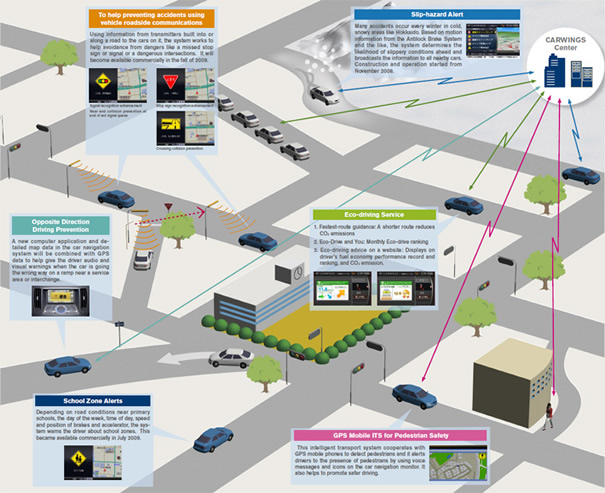
\includegraphics[scale=0.5]{Imagenes/cits}
		\caption[Ejemplo de algunos C-ITS]{Ejemplo de algunos C-ITS \protect\footnotemark}
		\label{fig:cits}
	\end{center}
\end{wrapfigure}
\footnotetext{https://www.nissan-global.com/EN/TECHNOLOGY/OVERVIEW/its.html}


Los sistemas inteligentes de transporte cooperativos, C-ITS (del inglés, \textit{Cooperative Intelligent Transport Systems}) (Figura \ref{fig:cits}), se definen como aquellos sistemas de seguridad, eficiencia y comodidad en el entorno vial, basados en el intercambio de información entre vehículos y/o insfrasestructura mediante comunicaciones inalámbricas. Incluso se puede extender al intercambio de información a usuarios que no están en el interior de un vehículo, es decir, el vehículo se encuentra conectado a un entorno cooperativo, lo que posibilita que además de poseer datos propios pueda obtener datos de su entorno.\\

\par  En pro de los avances en este área el 30 de noviembre del 2016 el Unión Europea adoptó la estrategia europea en C-ITS \footnote{https://ec.europa.eu/transport/themes/its/ } , iniciativa que tiene como objetivo facilitar la convergencia entre las inversiones y los marcos de trabajo en toda la EU, con la finalidad de poder ver estos sistemas para el 2019. En el mismo se pretende que en el 2018, se aseguren todos los aspectos legales para porporcionar certeza a los inversores públicos y privados, así como a distintos entes internacionales. Esta iniciativa consta de tres fases, siendo la primera (2014-2016), el acondicionamiento de las infraestructuras en las vías y prueba de las DSRC, la segunda (2016-2017), las primeras pruebas tangibles de estos sistemas en la sociedad y la tercera (2017-2019), la implementación definitiva de los mismos.\\

\par A través de los C-ITS se pueden realizar distintas maniobras cooperativas que pueden facilitar el trabajo en situaciones complejas, además de ayudar al conductor cuando el mismo no se encuentre en condiciones de poder reaccionar correctamente.           


\subsection{Maniobras Cooperativas}


Las investigaciones llevadas a cabo para el control de vehículos autónomos en maniobras cooperativas están en la vanguardia de los ITS. Ejemplos de estas son: maniobras de intersecciones, ACC, adelantamientos, platoonig, entre otras, descritas a continuación:

\subsubsection{ACC}

Permite fijar una velocidad de conducción y mantenerla de forma automática sin necesidad de la intervención del conductor, manteniendo una distancia de seguridad con el carro de adelante. Para poder calcular esta distancia se pueden emplear distintos dispositivos, como lo pueden ser radares, telémetros láser, o comunicaciones V2V, donde los vehículos transmiten su velocidad y posición  al resto de los vehículos \cite{van2006impact}. Cuando se emplean las comunicaiones V2V el ACC pasa a ser llamado control de crusero adaptativo cooperativo, CACC (del inglés, \textit{Cooperative Adaptative Cruise Control}) (Figura \ref{fig:acc2}) .\\  

\begin{figure}[!h]
	\centering
		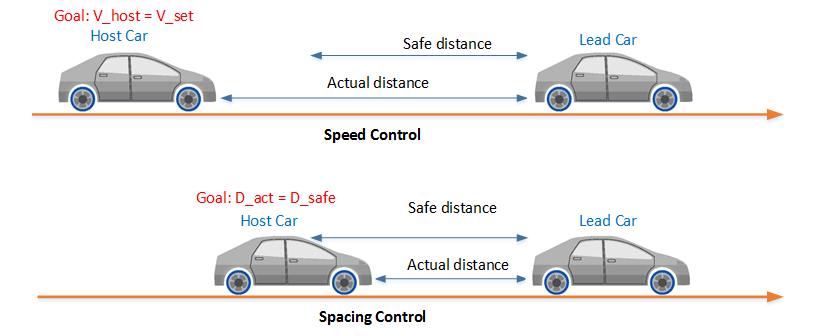
\includegraphics[scale=0.7]{Imagenes/acc2}
		\caption[Ejemplo de un CACC]{Ejemplo de un CACC \protect\footnotemark}
		\label{fig:acc2}
	\end{figure}	

\footnotetext{https://cecas.clemson.edu/cvel/auto/systems/DSRC.html}

\subsubsection{Stop And Go}

Permite acelerar y desacelerar los vehículos, cuando sea necesario, aumentando así el confort al manejar, seguridad del conductor y reducir los riesgos de colisiones. Para cumplir estos objetivos el vehículo toma acción sobre el acelerador y freno, por lo general en situaciones en el que el carro que está al frente realiza un frenado de emergencia o en momentos que se presente tráfico en la vía. Existen distintos métodos de predicción para saber cuando se debe frenar y cuando se debe acelerar, siendo las comunicaciones V2V, el método más efectivo, donde a través de la velocidad y posición del vehículo delantero se puede establecer un criterio de cuándo realizar estas acciones \cite{marzbanrad2015prediction}. En la figura \ref{fig:stg} se pueden apreciar los dos casos, cuando se frena (a) y cuando acelera (b).\\

\begin{figure}[!h]
	\centering
		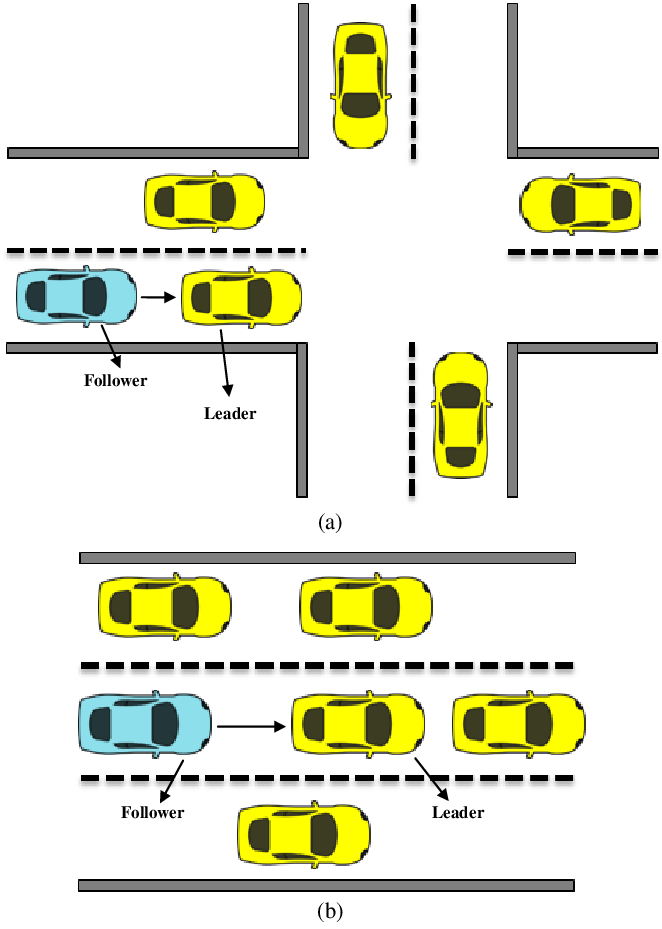
\includegraphics[scale=0.8]{Imagenes/stg}
		\caption{Ejemplo de un Stop and Go \cite{marzbanrad2015prediction}}
		\label{fig:stg}
	\end{figure}	

 
\subsubsection{Control Lateral}

Permite controlar el volante dependiendo de la posición del vehículo delantero, es decir controla el moviento lateral, tomando en cuenta las acciones del carro que tenga adelante, y de esta forma realizar la conducción del vehículo que permita al conductor descansar en momentos de mucho cansancio. Para lograr esta forma de conducción se emplean las comunicaciones V2V, en donde el vehículo delantero transmite su posición y dirección, para que el carro seguidor ajuste su posición con respecto a esta. En la figura \ref{fig:cl} se puede ver un ejemplo del control lateral en un cambio de canal.\\


\begin{figure}[!h]
	\centering
		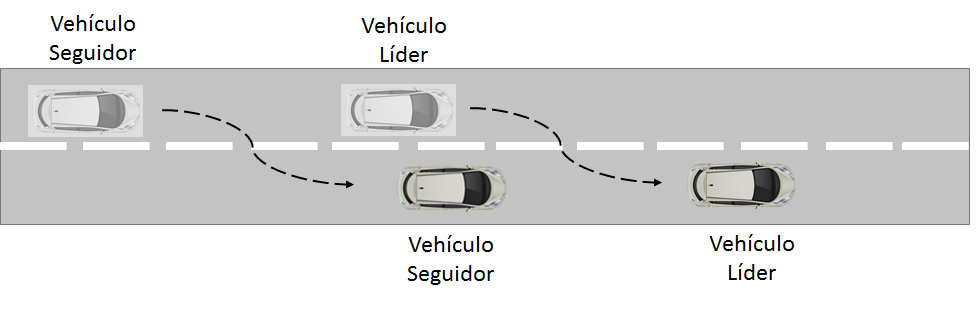
\includegraphics[scale=0.6]{Imagenes/cl}
		\caption{Ejemplo de un Contol Lateral}
		\label{fig:cl}
	\end{figure}	

 

\subsubsection{Platoonig}

Permite que un grupo de vehículos puedan viajar a una distancia segura, y a altas velocidades. En esta maniobra el carro líder fija la velocidad y dirección del grupo, enviándo mediante comunicación V2V, su velocidad, posición y dirección a los demás integrantes del grupo, para que los mismos se ajusten tomando como referencia estos datos. Con esta forma de conducción se reducen los riesgos de colisiones, así como una optimización de la cantidad de vehículos en las autopistas. En la Figura \ref{fig:plat} se puede apreciar un ejemplo de Platooning, donde el vehículo líder es un camión que guía a los demas carros.\\

\begin{figure}[!h]
	\centering
		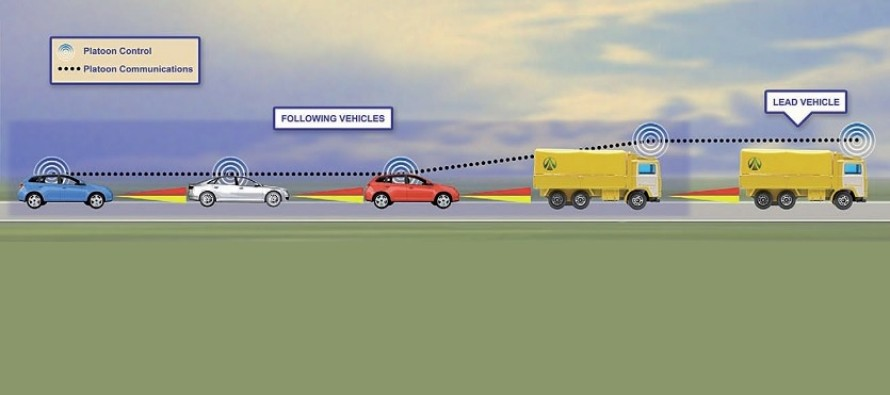
\includegraphics[scale=0.6]{Imagenes/plat}
		\caption[Ejemplo de un Platooning]{Ejemplo de un Platooning \protect\footnotemark}
		\label{fig:plat}
	\end{figure}	

 \footnotetext{http://www.driverlesstransportation.com/platooning-1157}


\section{Lógica Borrosa}

La lógica borrosa se puede definir como una lógica multivaluada que permite representar matemáticamente la incertidumbre y la impresición, proporcionando herramientas formales para su tratamiento. Básicamente, cualquier problema del mundo se puede resolver a través de un conjunto de variables de entradas, las cuales proporcionan un valor adecuado de variables de salidas. El término fue acuñado por primera vez en 1974 por Lofti A. Zadeh, donde la presentó como una forma de procesamiento de información en la que los datos podrían tener asociados un grado de pertenencia parcial a conjuntos. Además describió el concepto de conjunto difuso y su función de pertenencia asociada, la cual toma valores en el intervalo unitario, y siendo en la década de los 90 que se introdujeron los conceptos restantes, variable linguistica y de reglas if-then \cite{morcillo2011logica}.\\

\par Para que la lógica borrosa pueda lograr su objetivo, se establecen conjuntos difusos que proporcionan la imprecisión de forma cuantitativa al cual será sometido el valor. Dichos conjuntos se manifiestan a través de funciones de membresía o pertenencia las cuales entregan el grado de pertenencia de un valor hacia un tributo establecido.\\

\par Para ejemplificar mejor estos conceptos, se procederá a describir el caso de la altura en los hombres. Según la lógica clásica se definen dos conjuntos, hombres altos y hombres bajos, quienes se constituyen de hombres mayor a 1.8 m y menor a dicho valor, es decir cualquier hombre cuya estatura sea 1.79 m será considerado como bajo, y uno de 1.81 m, como alto. En la lógica difusa no solo se tienen dos conjuntos estrictamente definidos, si no que se tienen conjutos intermedios, los cuales permiten una transición entre un caso y el otro, es decir un hombre puede tener una estatura de 1.78 m con un grado de certeza de 0.8 y bajo con un grado de certeza de 0.2, mientras que en el caso de un hombre de 1.60 m de estatura, este puede pertenecer al conjunto de hombres bajos con 0.9 grados y al de hombres altos con 0.1 grados. Dicha comparación puede ser mejor apreciada en la figura \ref{fig:hombres}.\\

\begin{figure}[!h]
	\centering
		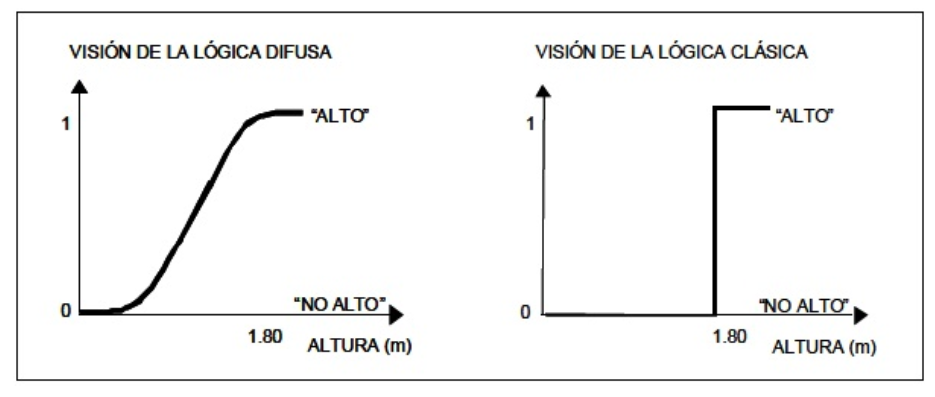
\includegraphics[scale=0.7]{Imagenes/hombres}
		\caption{Lógica clásica vs Lógica difusa \cite{fuzzy}}
		\label{fig:hombres}
	\end{figure}	

\subsection{Control Borroso}

Los controladores borrosos surgen en los años 60, como una herramienta empleada en el control de procesos complejos de cualquier tipo, permitiendo dar valores intermedios entre dos extremos a una variables que se desea manipular, y con esto hacer posible que la lógica humana sea empleada de manera directa.\\

\par Estos controladores reciben entradas analógicas debido a su rango no discreto y se clasifican por el grado de membresía de sus conjuntos, los cuales corresponden a reglas implementadas que aplican la lógica humana para determinar de que forma los conjuntos difusos o sus combinaciones, definen la(s) salida(s) del controlador. En la figura \ref{fig:fuzzy} se puede encontrar un esquema de la representación de estos controladores.\\ 

\begin{figure}[H]
	\centering
		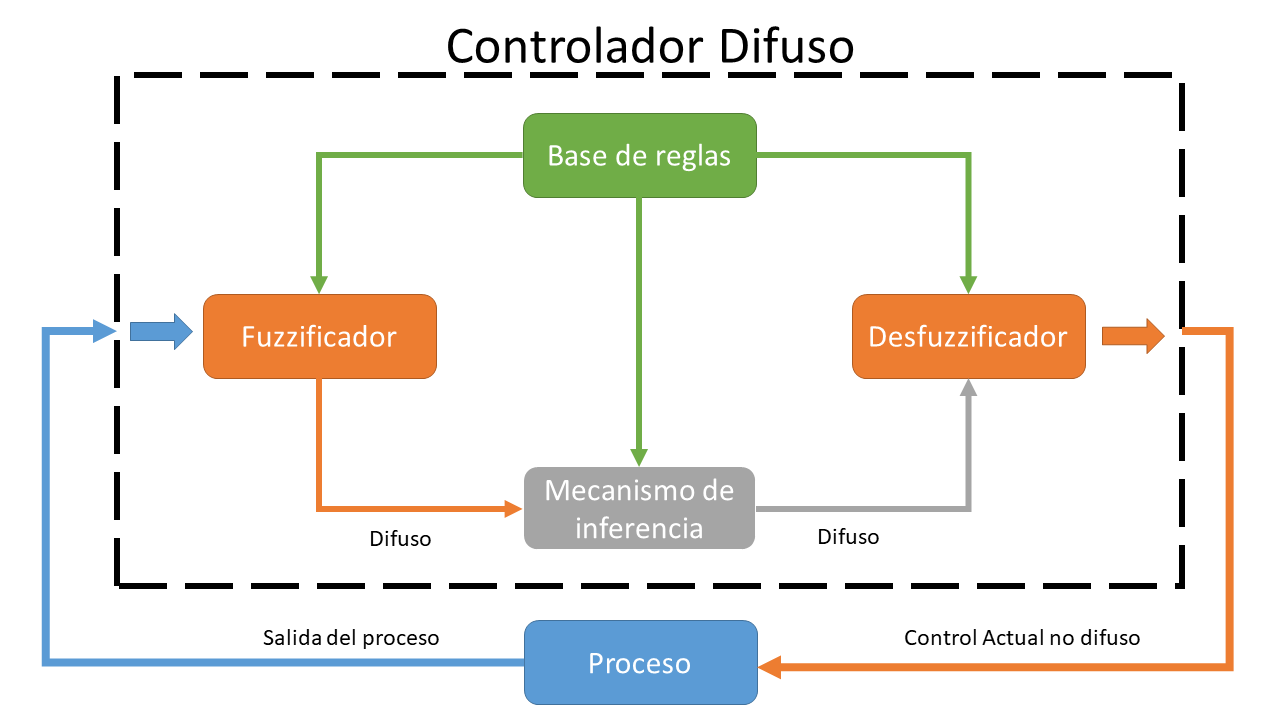
\includegraphics[scale=0.5]{Imagenes/fuzzy}
		\caption{Esquema de un controlador borroso}
		\label{fig:fuzzy}
	\end{figure}	

\par Como se puede apreciar los controladores borrosos están compuestos por varias etapas, los cuales consisten en \cite{fuzzy}:

\begin{itemize}
	\item Fuzzyficación: Esta estapa consiste en transformar la(s) variable(s) de entrada en un grado de pertenencia que cuantifica el grado de membresía de los determindos conjuntos difusos. Es en este proceso donde las funciones de membresía son aplicadas, más comunmente tienen foma de trapezoides, triángulos, gaussianas, etc. Definiendo de esta forma el grado de transición de pertenencia entre un conjunto y otro, permitiendo así, que la etapa de inferencia pueda interpretar la entrada de forma correcta 
	\item Inferencia: Es en esta etapa que se representa verdaderamente la lógica del controlador, es donde se evaluan las entradas "fuzzyficadas" de la etapa anterior, a través de condiciones definidas,  las cuales permiten calcular la salida del mismo. La base de reglas está constituida por una serie de condiciones que consideran la(s) entrada(s) y establecen cuantitativamente salidas difusas que posteriormente serán interpretadas por la etapa final. Dentro de esta fase se pueden encontrar dos métodos importantes, Mamdani y Takagi-Sugeno, que consisten en \cite{jang1996input}:
	\subitem Mamdani: es posiblemente el método más empleado, propuesto por Ebrahim Mamdani en 1975, este método busca obtener un único número que represente el resultado, a través de la evaluación de los grados de pertenencia en las reglas propuestas. En el caso de de que una regla tenga multiples antecedentes se utilizan los operadores AND u OR, dependiendo de lo que se busque, en el caso del operador AND se suele usar la T-Norma estándar del mínimo y para el OR la T-Conorma estándar del máximo. Finalmente con el resultado de esta evaluación se aplica un recorte o escalado a las funciones de salida para unificarlas, y así obtener el valor.
	\subitem Takagi-Sugeno: este método emplea los mismos principios que Mamdani, con la única diferencia que, para obtener el valor de salida no se emplean funciones de pertenencia, sino que se asignan valores númericos a las reglas, reduciendo el coste computacional con respecto a mandani, pero perdiendo la representación del conocimiento humano.     
	\item Desfuzzycación: Es la última etapa que realiza el controlador, es donde se estalece(n) la(s) salida(s) del mismo, a partir de las reglas evaluadas en la etapa procedente. Dependiendo del método de inferencia empleado se pueden utilizar técnicas como el centro de gravedad o centro promediados para el caso de Mamdani, o funciones ponderadas para el caso de Takagi-Sugeno.    
\end{itemize}


\section{Resumen}

En el presente capítulo se presenta el estado del arte, donde primero se resumieron algunos puntos de importancia para entender, cómo están estructurados los sistemas de comunicaciones actualmente, como lo son el modelo de capas OSI y las redes ad-hoc, así como tambien los protocolos de transporte que se emplean hoy en día.\\

\par De igual forma se presentó una descripción extensa de los protocolos de comunicación, tanto vehiculares, como comerciales. Donde también se explicó el cómo surgió cada uno, sus componentes y sus usos.\\

\par Finalmente se mencionaron los C-ITS y de cómo estos pueden ayudar con distintos problemas que se presentan a la hora de conducir. Para luego dar a conocer algunas maniobras que se pueden realizar con estos sistemas, más específicamente las que se realizaron en este trabajo, y para cerrar se describieron los fundamentos sobre los cuales estan basados los controladores borrosos, controladores empleados para el desarrollo de las maniobras cooperativas presentadas.      







%%Arquitectura de Control
\chapter{Plataformas Experimentales}\label{sec:capitulo4}
\thispagestyle{empty}
En este capítulo se explican las plataformas experimentales utilizadas para el desarrollo y validación de los algoritmos propuestos en el presente trabajo, las cuales fueron: Matlab y Dynacar. Donde la herramienta de Matlab fue empleada para la realización de los códigos,  y conjunto a su entorno de simulación, Simulink se implementaron los bloques que conforman la arquitectura de control de los vehículos, más específcamente los relacionados a las comunicaciones V2V y maniobras cooperativas, para luego ser utilizdos y validados en el simulador Dynacar. Es por esto que a continuación se detallará de mejor forma cada una de estas plataformas.\\
\section{Software Matlab}
MATLAB\footnote{https://la.mathworks.com/products/matlab.html/} es una herramienta de software matemático que ofrece un entorno de desarrollo integrado, IDE (del inglés, \textit{Integrated Development Environment}), que cuenta con diversas prestaciones como la manipulación de matrices, implementación de algoritmos, creación de interfaces gráficas de usuario, GUI (del inglés, \textit{Graphical User Interface}) y la comunicación con programas en otros lenguajes y otros dispositivos de hardware. Debido a su capacidad de desempeño asíncrono permite manejar fuentes heterógeneas de datos, como sensores, sistemas de comunicación, etc, sin nunguna restricción. Teniendo en cuenta estas cualidades, el MATLAB permite a ingenieros e investigadores utilizar las ventajas de un software eficiente y fácil de usar en aplicaciones que necesitan desarrollos rubustos y de procesamiento rápido.\\
\par En este trabajo se empleó la versión 2016a \footnote{https://la.mathworks.com/company/newsroom/mathworks-announces-release-2016a-of-the-matlab-and-simulink-product-families.html/} de MATLAB, disponible desde el 21 de marzo de 2016, la cual cuenta con numerosas mejoras con respecto a sus antecesoras, como por ejemplo: la inclusión y correción de distintos toolbox relacionados al área de control, así como también el perfeccionamiento en las técnicas de depuración de código. Este IDE posee cuatro ventanas, como se muestra en la figura \ref{fig:ide}.\\

\begin{figure}[!h]
	\centering
		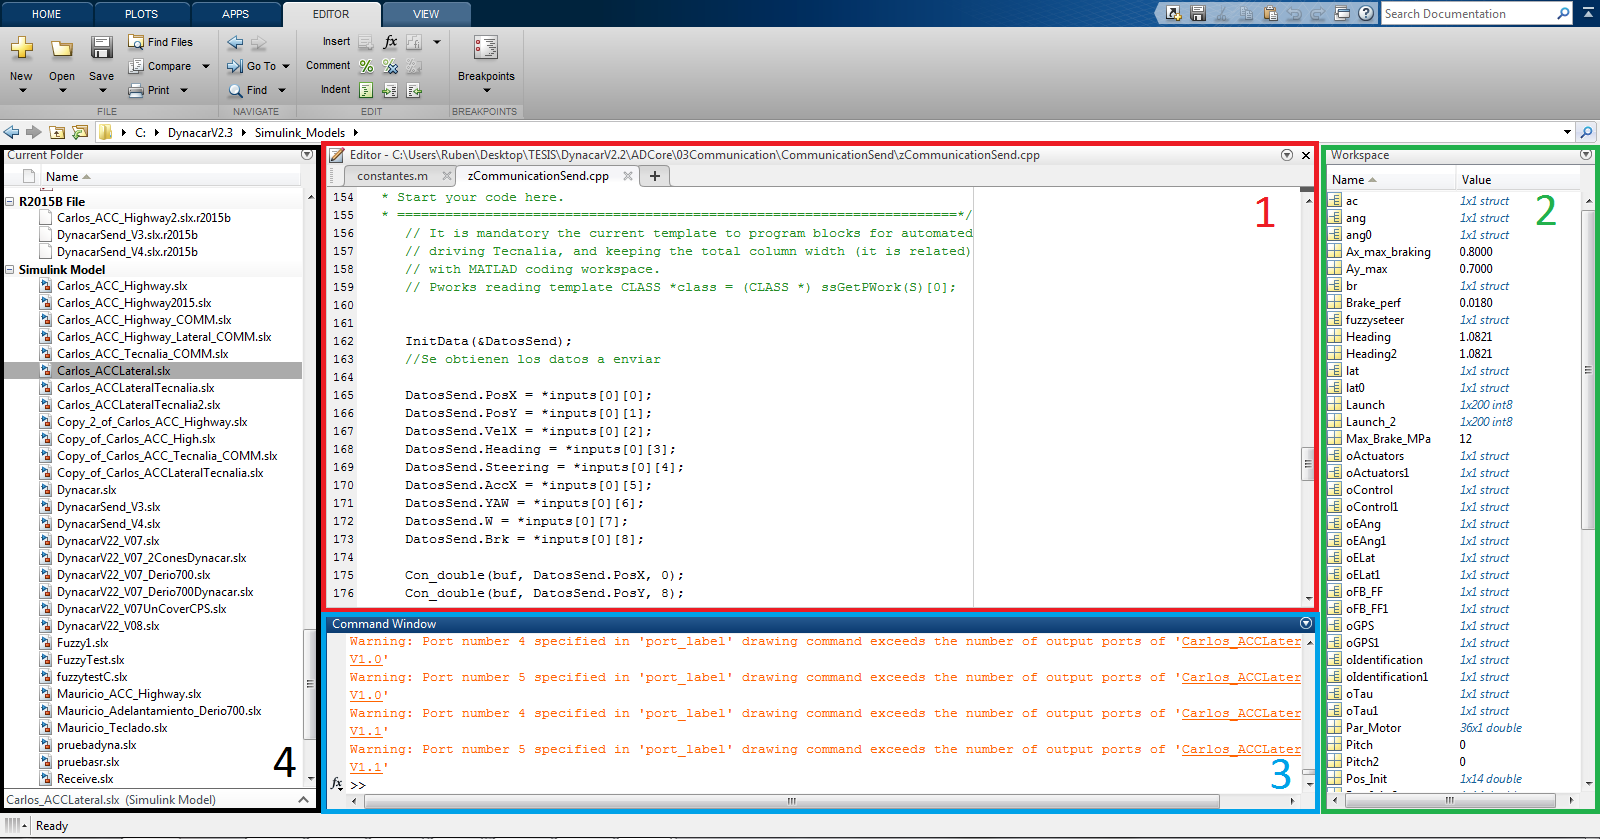
\includegraphics[scale=0.3]{Imagenes/ide}
		\caption{IDE de MATLAB}
		\label{fig:ide}
\end{figure}	 
\par Donde:\\
\begin{enumerate}
    \item Editor de texto: es donde se crean programas y funciones, para luego ser compiladas y ejecutadas. 
    \item Espacio de trabajo: es donde se muestran todas las variables y estructuras creadas, las cuales pueden ser manipuladas tanto con la ventana de comandos como con el editor de texto.
    \item Ventana de comandos: es donde se pueden escribir y ejecutar líneas de código directamente.
    \item Carpeta actual: es donde se muestra la carpeta actual, con sus respectivos archivos.
\end{enumerate}
\par Este software emlea su propio lenguaje de programación, el lenguaje M, pero a través de compiladores como Mingw32, se pueden utilizar otros lenguajes como C o C++. Lo que da paso a la utilización de otras características como lo son el uso de las S-Function, funciones de suma importancia en el esquema de Dynacar, ya que permiten crear bloques de simulink, empleando algoritmos realizados en lenguajes como C, C++ y Fortran.\\
\par Para la realziación de los bloques del sistema de comunicación se empleron las S-Function, conjunto a la libreria de Sockets para Windows de lenguaje C. Libreria que permite el uso de los sockets, que son enlaces punto a punto, que permiten comunicar una computadora con otra. Dichos enlaces pueden ser de dos tipos: Stream Sockets y Datagram Sockets, siendo basados cada uno en los protocolos de trasnporte TCP y UDP respectivamente. Ya habiendo explicado el software MALTAB, ahora se procederá a descrbir la herramienta, Simulink
\subsection{Simulink}
Simulink es una herramienta de MATLAB hecha para modelar, simular y analizar sistemas dinámicos. Soporta tanto sistemas lineales como no lineales, modelando tiempo continuo, tiempo discreto o en forma mixta. Estas características resultan favorables para la implementación de la arquitectura de control por medio de bloques. En la figura \ref{fig:sim} se puede ver la interfaz gráfica de Simulink, interfaz que se basa en una amplia biblioteca de componentes con entradas y salidas que se pueden interconectar entre sí. Este editor gráfico permite crear y gestionar bloques jerárquicos, es decir se puede tener diagrama principal y dentro del mismo tener diagramas secundarios, cualidad de gran utilidad para la independización de los módulos de comunicación.\\ 

\begin{figure}[!h]
	\centering
		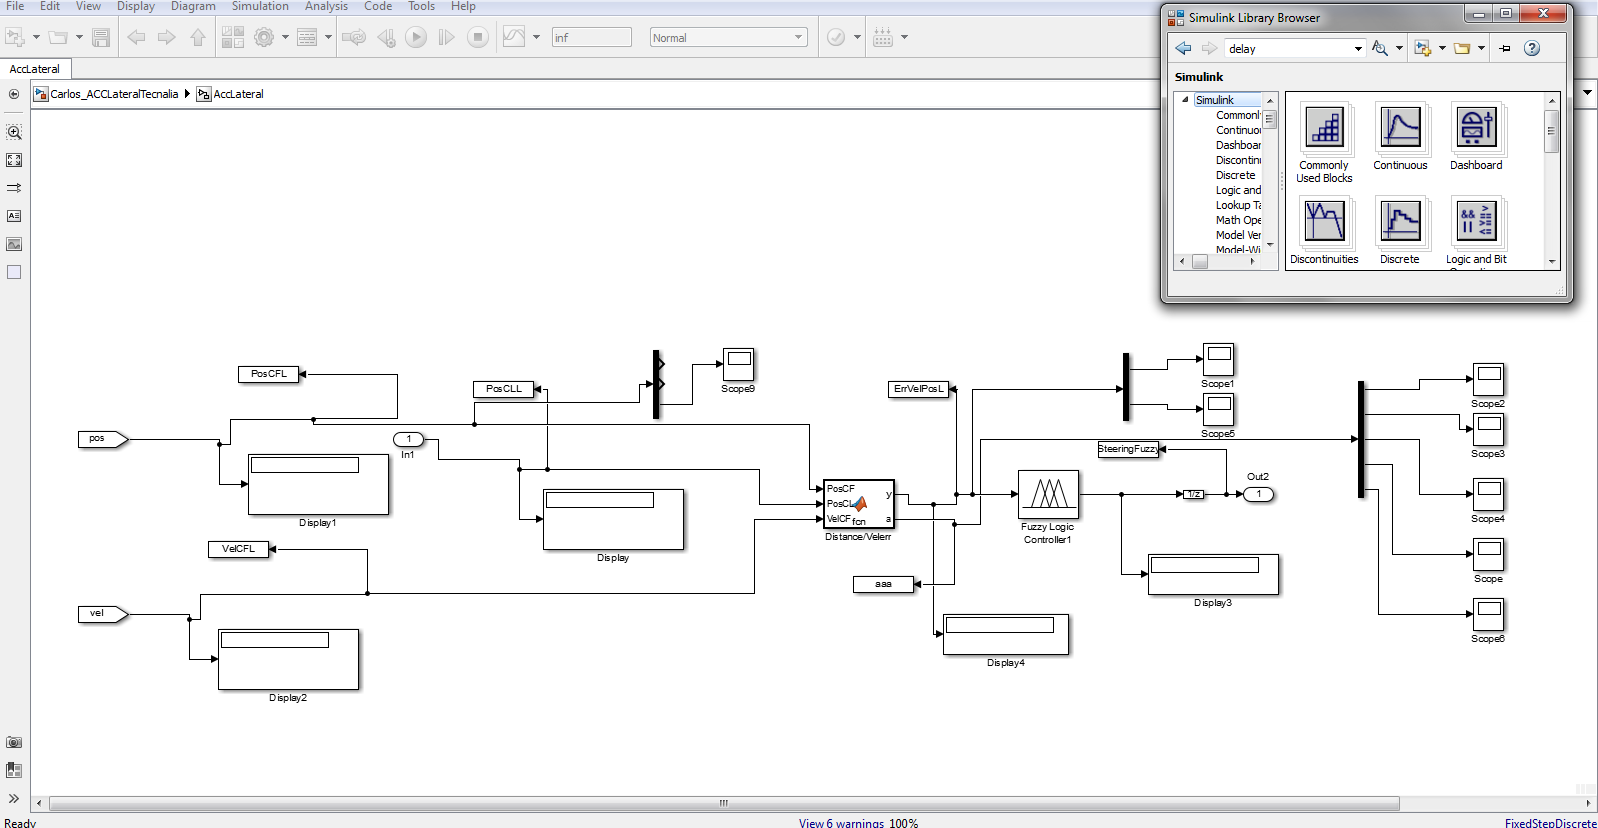
\includegraphics[scale=0.3]{Imagenes/sim}
		\caption{IDE de Simulink}
		\label{fig:sim}
\end{figure}	
\section{Simulador Dynacar}
Dynacar\footnote{http://www.dynacar.es/en/home.php es software}, desarrollado por Tecnalia en la pataforma de LabVIEW, es un software que permite a los ingenieros diseñar y probar modelos completos de vehículos en un ambiente completo y personalizable. Dynacar está compuesto de tres módulos:
\begin{itemize}
	\item Código de la dinámica de vehículos en LabVIEW: son los agoritmos necesarios para el software de prueba, los mismos son ejecutables en tiempo real, y poseen ya, una biblioteca de carros y escenarios de prueba básicos.
	\item Interfaz gráfica de usuario: es la interfaz que permite realizar la parametrización de los vehículos y escenarios (Figura \ref{fig:ste}).
	\item Entorno visual 3D: es el módulo que permite la visualización de las pruebas y del simulador de manejo real del vehículo en el entorno virtual.
\end{itemize}

\begin{figure}[!h]
	\centering
		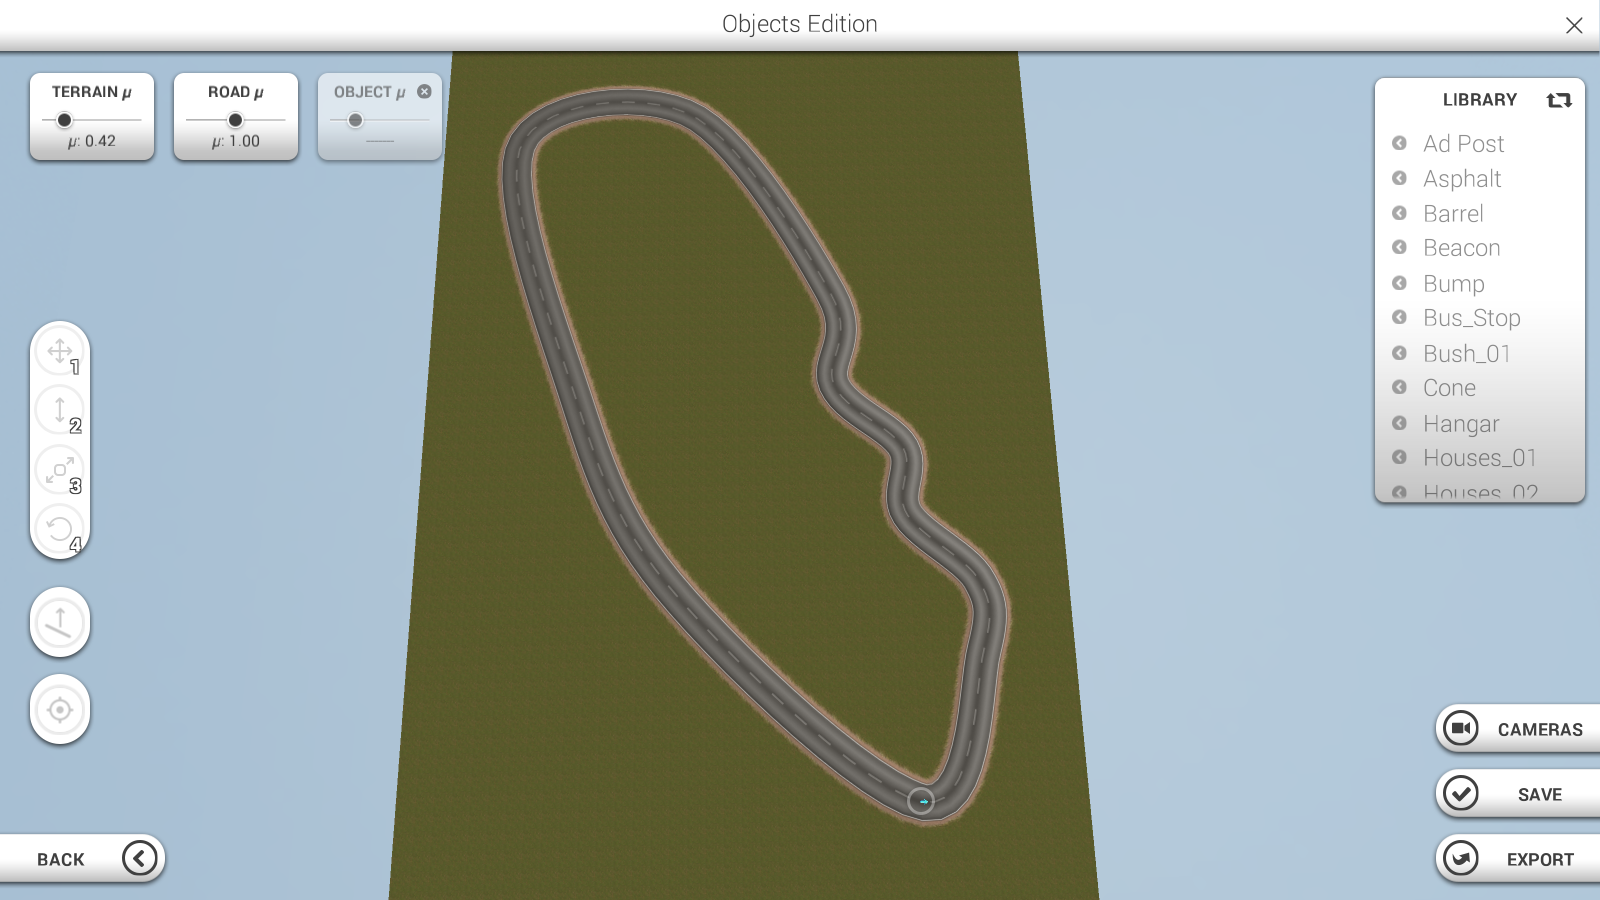
\includegraphics[scale=0.3]{Imagenes/ste}
		\caption{Interfaz gráfica de usuario para la creación de escenarios}
		\label{fig:ste}
\end{figure}	


\par Para poder modelar los vehículos en el simulador, es necesario aportar los siguientes datos:

\begin{itemize}
	\item Masa del vehículo e inercia.
	\item Parámetros de suspensión.
	\item Propiedades de la derección del vehículo.
	\item Características de la aerodinámicas del vehículo.
	\item Propiedades de los neumáticos.
	\item Motor, caja de cambios y propiedades de la transmisión.
	\item Detalles de los actuadores.
\end{itemize}
\par Este simulador se hizo con el objetivo de poder detectar fallos en la ejecución de las maniobras de forma sencilla, y de esta manera poder conocer cuáles son los aspectos que se necesitan ser revisados. Para conseguir este objetivo la plataforma ofrece el entorno visual, el cual se comunica mediante socket de UDP con otras aplicaciones, las cuales envían una trama de datos, con las características del vehículo. En dicho entorno se pueden observar en tiempo real la velocidad lineal en Km/h y la velocidad angular en RPM las ruedas. Además de de estos datos también muestra las acciones sobe los actuadores medidos en porcentajes,junto con la dirección de los vehículos, como se puede apreciar en la Figura \ref{fig:simu}.\\\\\\\\   

\begin{figure}[!h]
	\centering
		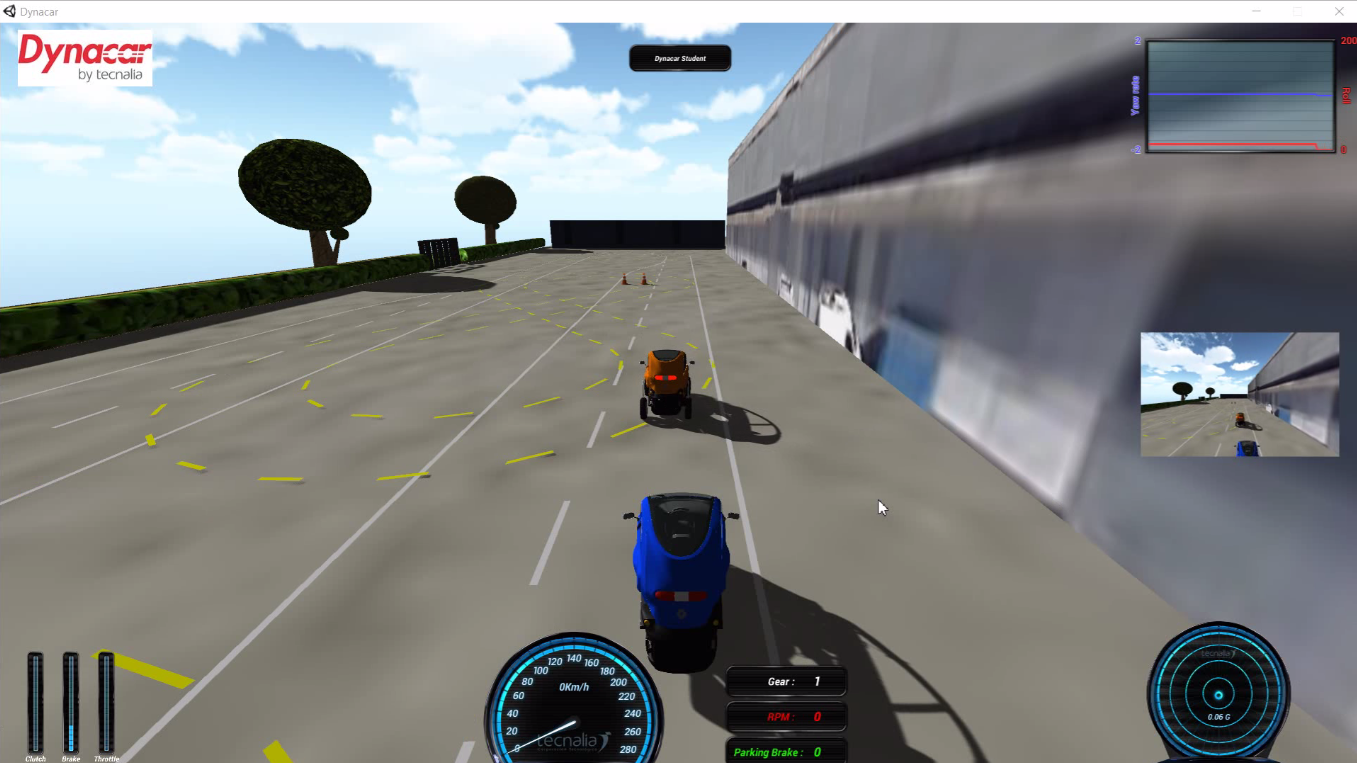
\includegraphics[scale=0.45]{Imagenes/simu}
		\caption{Simulador Dynacar}
		\label{fig:simu}
\end{figure}	

\subsection{Plataformas de Prueba}

A continuación, se presenta una breve descripición de la automatización e instrumentación del Twizy, que corresponde a la plataforma real, así como una explicación de la plataforma virtual, a través de modelos matemáticos.

\subsubsection{Plataforma Real}

Como fue comentado en la sección 2.2.1 para las pruebas reales se emplea el Renault Twizy 80, un vehículo eléctrico, capaz de alcanzar una velocidad máxima de 80 Km/h, el cual ha sido instrumentado de tal forma que el control del volante y de los pedales es realizado a través de una red de bus CAN. Una descripción más detallada de las características físicas del vehículo se puede encontrar en la tabla \ref{tab:cart} \cite{twizyman}\\

\begin{table}[H]
  \centering
\resizebox{\textwidth}{!}{
    \begin{tabular}{|p{16.93em}|c|}
    \toprule
    \multicolumn{1}{|c|}{Características} & Valores \\
    \midrule
    Masa (Kg) & 611.500 \\
    \midrule
    Centro de gravedad X, Y, Z (m) & -0.928, 0, 0.488 \\
    \midrule
    Ancho entre ruedas (m) & 1.686 \\
    \midrule
    Distancia entre el centro de las ruedas delanteras con las traseras & 1.094 \\
    \midrule
    Inercia Ix, Iy, Iz (Kg-m2) & 243.175, 430.166, 430.166 \\
    \midrule
    Radio de las ruedas delanteras (m) & 0,265 \\
    \midrule
    Radio de las ruedas traseras (m) & 0,281 \\
    \midrule
    Torque máximo (N-m) & 57 \\
    \midrule
    Caballos de fuerza (hp) & 11 \\
    \bottomrule
    \end{tabular}}%
  \caption{Características físicas del Twizy 80}
  \label{tab:cart}%
\end{table}%



\par Esta plataforma se puede dividir en tres sistemas manejados por diferentes dispositivos electrónicos y actuadores (Tabla \ref{tab:sen}), los cuales son controlados por un PLC \cite{marcanolow}:

\begin{itemize}
\item Volante: es manejado por un motor de paso, el cual es controlado por señales moduladas por ancho de banda, PWM (del inglés, \textit{Pulse-Width Modulation}). 
\item Acelerador: es controlado por la unidad de control del motor, ECU (del inglés, \textit{Engine Control Unit}), la cual recibe una señal de voltaje analógica entre 0 y 10 VDC. 
\item Freno: es manejado a través de un actuador mecánico lineal.
\end{itemize} 

% Table generated by Excel2LaTeX from sheet 'Hoja1'
\begin{table}[H]
  \centering
\resizebox{\textwidth}{!}{
    \begin{tabular}{|c|c|}
    \toprule
    Data de la Inercia y Posición & \textit{GNSS-aided IMS + Base Station} \\
    \midrule
    OBU   & Fanless - i7-6700TE - 32 GB RAM \\
    \midrule
    \multirow{2}[4]{*}{Sistema de Frenado} & Actuador Lineal - 750 N \\
\cmidrule{2-2}          & Driver de 20 A del Motor DC \\
    \midrule
    \multicolumn{1}{|c|}{\multirow{3}[6]{*}{Sistema del Volante}} & Motor paso a paso híbrido de alto torque \\
\cmidrule{2-2}          & Encóder magnético con CANopen \\
\cmidrule{2-2}          & Driver de 20-80 V del motor paso a paso \\
    \bottomrule
    \end{tabular}}%
  \caption{Sensores y dispositivos electrónicos}
  \label{tab:sen}%
\end{table}%

\subsubsection{Plataforma Virtual}

Dynacar, además del ya descrito Visor 3D, incorpora un modelo multi-cuerpo \cite{cuadrado2013multibody} con el cual se pueden representar los vehículos virtualmente. Dicho modelo hace uso de de coordenadas relativas, así como también ecuaciones semi-recursivas del movimiento, basado en la transformación de la velocidad. Las suspensiones son consideradas como macro-articulaciones, cuyo comportamiento es descrito usando las estructuras de tablas de consulta.\\ 

\par Como se puede apreciar en la figura \ref{fig:mult}, las coordenadas cartesianas del chasis se encuentran en el medio del ancho de las ruedas delanteras (C), los ángulos de navegación  que proveen la orientación de las reudas con respecto al chasis se encuentran en los nudillos (K), y por último, las expresiones cinemáticas para las macro-articulaciones consideran, tanto la posición, como la velocidad y aceleración de las ruedas (W).\\

\begin{figure}[!h]
	\centering
		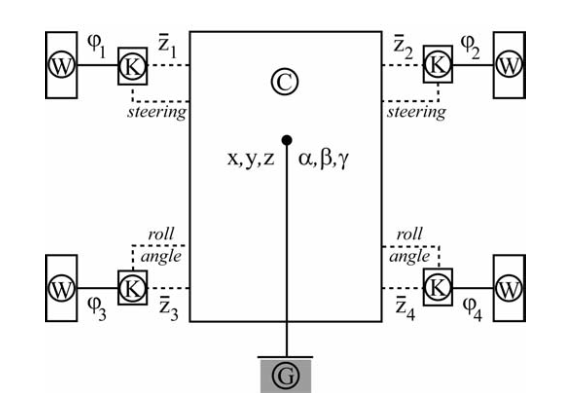
\includegraphics[scale=0.7]{Imagenes/mult}
		\caption{Modelo multi-cuerpo de Dynacar \cite{cuadrado2013multibody}}
		\label{fig:mult}
\end{figure}	      


\subsection {Arquitectura de control}
La arquitectura de control utilizada está compuesta por seis bloques representativos de cada módulo de interés dentro de la conducción automatizada (Figura \ref{fig:fram}), estos son: Adquisición, Percepción, Control, Comunicación, Desición y Actuación. Esta arquitectura ha sido utilizada en distintas aplicaciones de conducción autónoma, como por ejemplo, en \cite{lattarulo2017complete} y \cite{sriranjanlateral}. Siendo en el primero, usada para probar distintas metodologías, con el fin de validar distintos algoritmos de control y de planificación de ruta, mientras que para el segundo es implementada en autentificación de distintos algortimos de control lateral. Cada módulo es detallado a continuación:

\begin{figure}[!h]
	\centering
		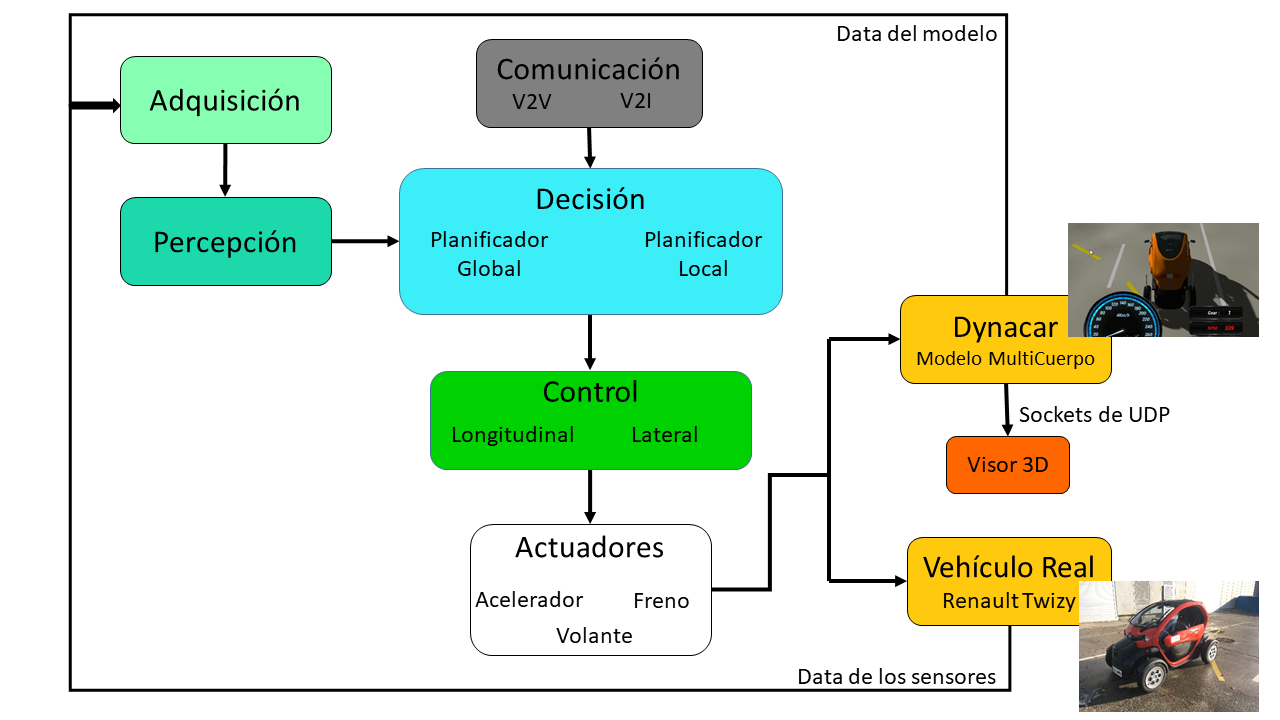
\includegraphics[scale=0.4]{Imagenes/fram}
		\caption{Arquitectura de control}
		\label{fig:fram}
\end{figure}	

\begin{itemize}
	\item Adquisición: es el bloque responsable de generar las señales de posición, velocidad, y demás información referente a la dinámica del vehículo. Estos datos son obtenidos a través del modelo multi-cuerpo que representa el vehículo simulado. En el caso de los vehículos reales este bloque reune y realiza las tareas de pre-procesamiento de la información proveniente de distintos dispositivos, como lo son: los distintos sensores, la unidad de medición inercial, IMU (del inglés, \textit{Intertial Measurement Unit}), el GPS diferencial, entre otros.  
	\item Comunicación: es el módulo encargado de simular las comunicaciones V2X, característica importante para la prueba de maniobras más complejas. Esta plataforma es de gran utilidad para simular las interacciones de los vehículos con las infraestructuras. En este bloque se enfocó el presente trabajo, incorporando a la arquitectura un bloque para enviar la trama de datos, la cual consta de la posición,velocidad, ángulo de dirección, tiempo y el valor de los actuadores, así como un bloque de recepción de datos. Además de los ya mencionados se agregó un bloque con el cual se puede observar en el visor 3D, el vehículo con el cual se esta realizando la comunicación.    
	\item Percepción: es el módulo responsable de recolectar la data de los módulo de adquisición, armando así un paquete con la información y los parámetros de configuración del vehículo, el cual es trasladado a los bloques de decisión y control. Dentro de la información a envíar, se pueden destacar: la estimación del ego-vehicle, la detección y/o clasificación de objetos, detección de carril, y la detección de señales de tráfico. 
	\item Decisión: es el bloque encargado de generar la ruta por donde se va a transitar, para lo cual el módulo se divide en dos sub módulos, el planificador global y el planificador local.
	\begin{itemize}
	\item Planificador global: es el encargado de generar la ruta que va a seguir el vehículo (Figura \ref{fig:gp}). Para crear la ruta el bloque considera la información tanto del punto de partida como del punto de llegada, así como también la información proveniente del bloque de HMI, que puede cambiar el camino de forma dinámica. Esta ruta tiene que ser lo suficientemente precisa para que el planificador local pueda generar trayectoria suave, que, además tome en cuenta escenarios urbanos, como intersecciones, rotondas, etc.

\begin{figure}[!h]
	\centering
		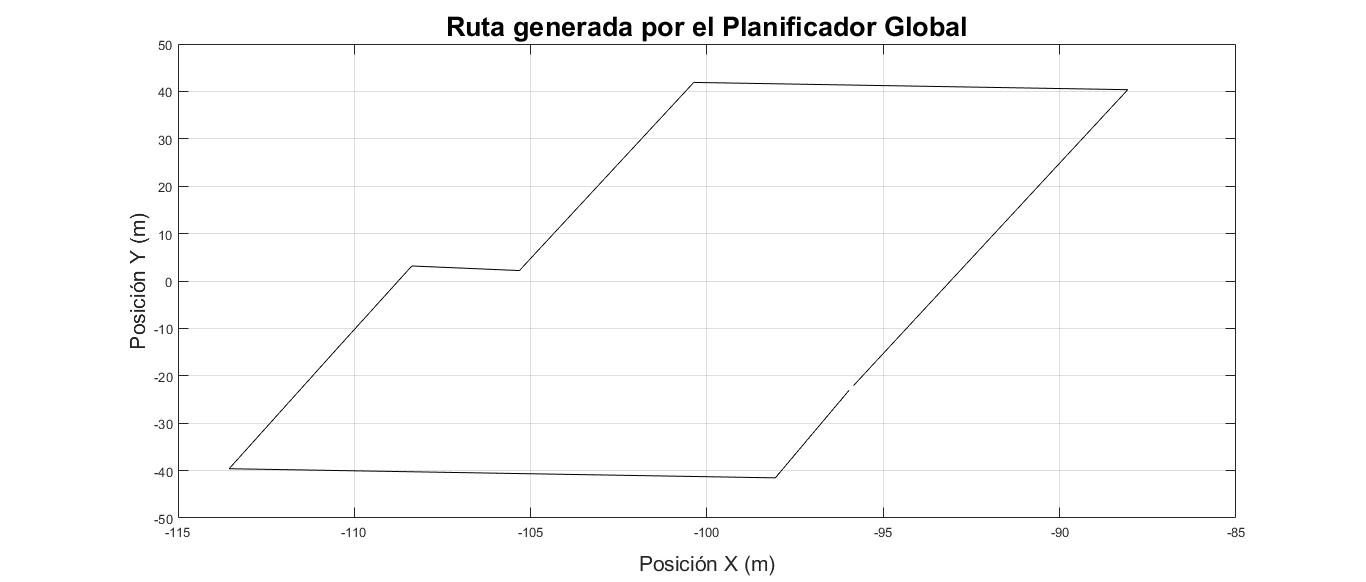
\includegraphics[scale=0.45]{Imagenes/gp}
		\caption{Ejemplo de una ruta generada por el Planificador Global.}
		\label{fig:gp}
\end{figure}	      

	\item Planificador local: basado en la información proveniente del planificafor global, este bloque genera una trayectoria suave empleando curvas paramétricas (Figura \ref{fig:pl}), como es demostrado en \cite{rastelli2014dynamic}. El objetivo es suavizar el cambio de la curvatura entre segmentos rectos y curvas. Este bloque considera la posibilidad de cambiar la trayectoria en caso de que ocurra un escenario ineseperado, como, evasión de objetos, incorporación, entre otros. Para generar este suavizado se emplean por ejemplo las curvas de bezier, como es demostrado en \cite{gonzalez2016review}, las cuales son de fácil implementación y de bajo coste computacional.

\begin{figure}[!h]
	\centering
		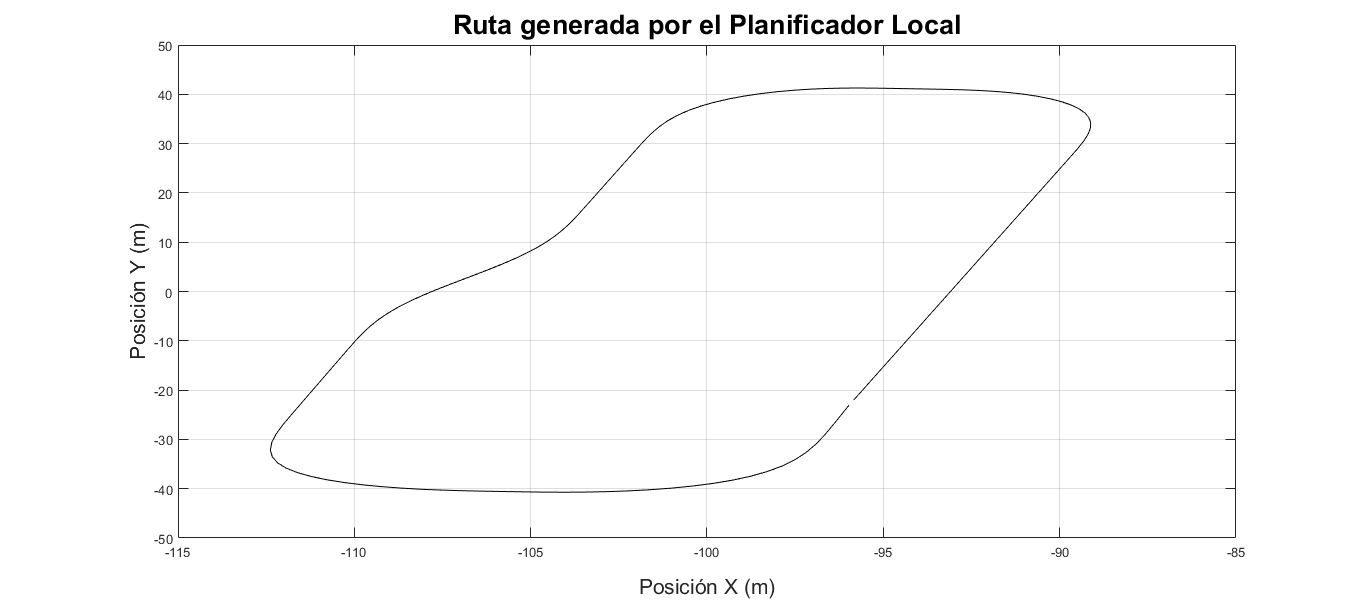
\includegraphics[scale=0.45]{Imagenes/pl}
		\caption{Ejemplo de una ruta generada por el Planificador Local.}
		\label{fig:pl}
\end{figure}	      

	\item \textit{ Buffer} de planificación: es el arreglo empleado para comunicar el bloque de desición con el de control. El mismo pretende optimizar e incrementar el tiempo de respuesta del cálculo de las leyes de control, en caso de detectarse una trayectoria irreal, como un generada con un objeto en frente del vehículo, la mismas es removida antes de enviarse al módulo de control. El \textit{Buffer} está compuesto por: el valor de identificación del punto, tipo de punto, coordinadas X-Y, máxima velocidad del segmento, curvatura y la orientación del segmento.    
	\end{itemize}
	\item Control: es el bloque encargado de realizar el control longitudinal (aceleración y freno) y el control lateral (Volante). Para cumplir este objetivo el módulo recibe el \textit{buffer} de planificación del bloque de desición, con el cual se puede emplear un controlador PID para el control longitudinal, y un controlador basado en la lógica difusa como el mostrado en \cite{perez2013trajectory}, para el control lateral, basado en la utilización del error lateral y error angular. 
	\item Actuadores: es el bloque encargado de normalizar las salidas del módulo de control, con el fin de poder tener señales de acción reales sobre el acelerador, freno y volante. Estas señales son posteriormente enviadas a los respectivos módulos de el vehículo real (actuadores) y virtual (modelo multicuerpo).
\end{itemize} 

\par En la figura \ref{fig:dyna} se puede apreciar la implementación de esta arquitectura en la herramienta Simulink, donde se observan los bloques bien divididos, con sus respectivas conexiones. De este diagrama se resalta el bloque de DynacarJam, el cual es el puente entre el diagrama y el visor 3D, ducho bloque recibe el valor de los actuadores y del volante, entregando un vector con todos los valores necesarios para el movimiento del vehículo en el simulador, siendo el equivalente, el bloque de Twizy V1.0, el cual cumple la función de puente entre Simulink y el vehículo.  	
   
\begin{figure}[!h]
	\centering
		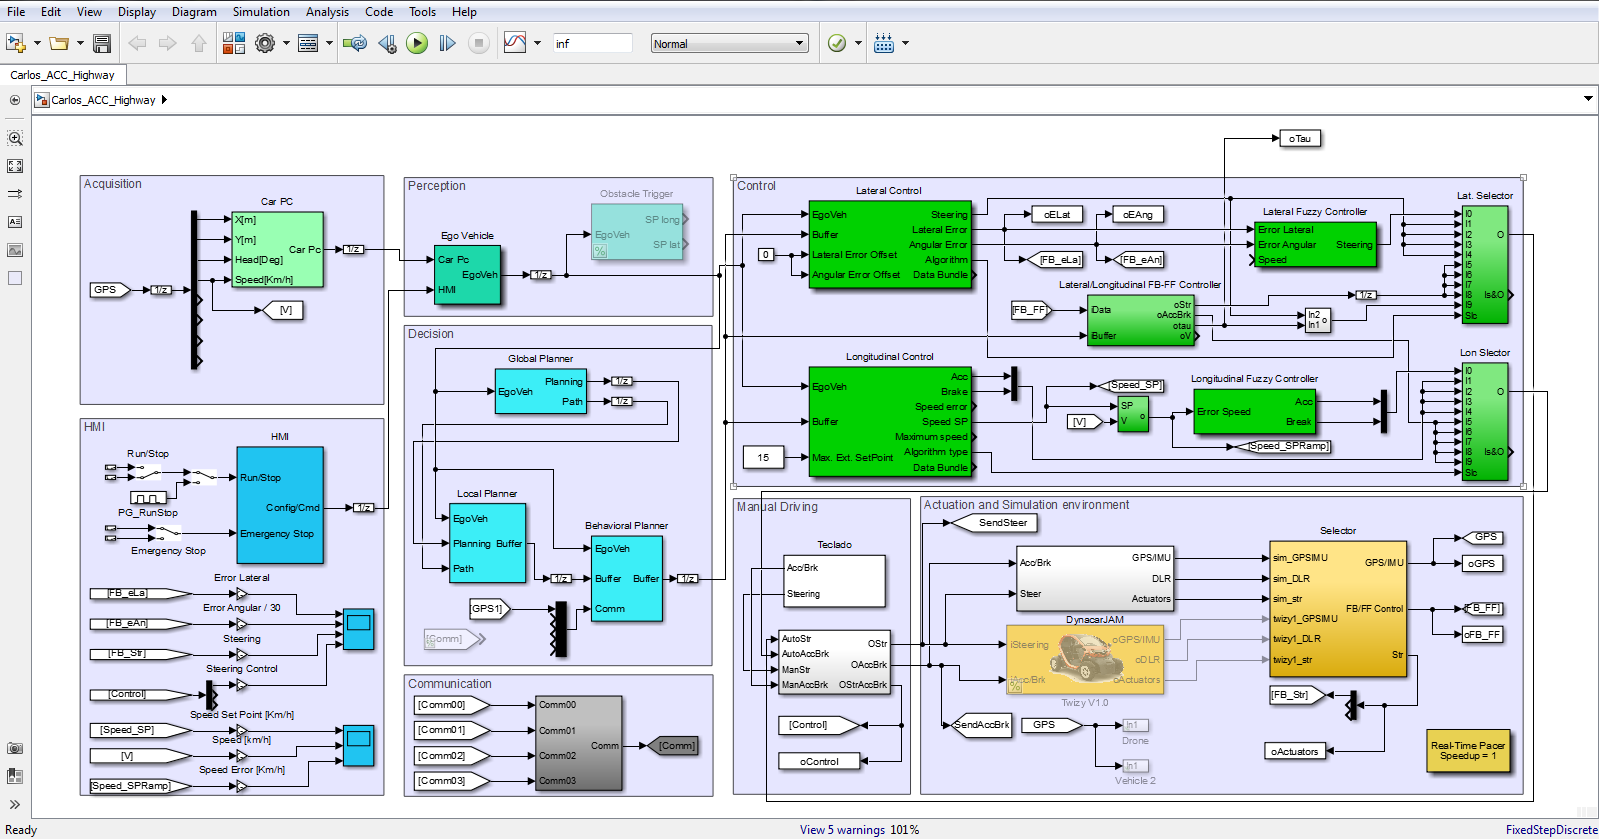
\includegraphics[scale=0.35]{Imagenes/dyna}
		\caption{Arquitectura de control implementada en Simulink}
		\label{fig:dyna}
\end{figure}	
\section{Resumen}
En el capítulo 4 se presentaron las plataformas experimentales empleadas en el transcurso del trabajo. Dentro de estas plataformas se encuentra MATLAB, del cual se resaltaron sus características más importantes, así como los beneficios de poder programar en otros lenguajes. Posteriormente se habló sobre la herramienta Simulink, que debido a su cualidad asíncrona se adapta perfectamente para implementar la arquitectura de control, tanto para el simulador Dynacar, como para los vehículos Twizy. Además, se presentó el simulador Dyancar como una forma de validar los algoritmos propuestos y los sistemas diseñados para vehículos autónomos. Cabe destacar que el mismo provee un entorno 3D, de gran utilidad para monitorear en tiempo real la respuesta de los vehículos en distintas situaciones, así como sus características.\\
\par Finalmente se presentó de forma muy breve la arquitectura de control establecida para la validación de los modelos, en el simulador Dynacar, describiendo cada bloque, así como las conexiones entre cada uno. Además se mostró la implementación de esta arquitectura en Simulink, resaltando la diferencia entre el diagrama empleado en Dynacar y el utilizado en los Twizy.     


%%Plataformas experimentales
\chapter{Sistema de Comunicación}\label{sec:capitulo5}
\thispagestyle{empty}

%\section{Desarrollo del Sistema de Comunicación}
%\subsection{S-Function}
%\subsection{Librería de Socket}
En el presente capítulo se describe el sistema de comunicación implementado en el simulador Dynacar, describiendo la composición de cada bloque, de envío, de recepción y de envío al visor 3D, así como la prueba del mismo a distintas tasas de envío, tanto haciendo uso del visor, como sin hacer uso de este, y de esta forma comprobar si el sistema es válido para las situaciones presentadas.\\

\par No obstante, primero se darán las razones por las cuales se optó por el sistema de comunicación comercial en vez, del vehicular, comparando los estándares de cada uno, y los beneficios que pueda tener uno sobre el otro, en las condiciones presentes en Tecnalia. Posteriormente se tocará el tema de los protocolos de transporte, con el objetivo de conocer cual es el más idóneo para el presente trabajo, para finalmente realizar una descripicón detallada del mensaje a enviar.  


\section{Análisis del Sistema de Comunicación}
Debido a lo complicado y costoso que puede llegar a ser desarrollar un sistema de comunicación vehicular, el presente trabajo propone una alternativa que consiste en emlpear elementos comerciales para realizar las conexiones entre los carros. Sin embargo, como se expuso anteriormente las comunicaciones vehiculares son complejas y requieren de que se cumplan una cierta cantidad de condiciones para efectuarse de manera efectiva, es por esto, que a continuación se compararán ambos sistemas con el fin de demostrar que en ciertos escenarios se puede emular la comunicación vehicular con sistemas comerciales.

\subsection{Sistema de Comunicación Comercial Vs Sistema de Comunicación Vehicular}

Los sistemas de comunicación vehicular hacen uso de los estandares ITS-G5 en Europa. ITS-G5, basan sus capas físicas y MAC en el estándar IEEE 802.11p, descrito en el capítulo 3. A su vez, la norma IEEE 802.11p está realizada bajo la convención IEEE 802.11a, también descrita en el capítulo 3. Ambos estándares emplean la técnica de transmisión OFDM, con la principal diferencia que la IEEE 802.11p hace uso de un ancho de banda de 10 MHz para cada canal, siendo este la mitad que el de IEEE 802.11a. Dicho cambio tiene como finalidad, hacer el sistema más robusto ante el desvanecimiento de las señales, así como aumentar la tolerancia ante los efectos de las señales multitrayecto, que se pueden presentar en los ambientes vehiculares \cite{lin2010comparison}. Las demás diferencias, con respecto a la capa física se pueden encontrar listadas en la tabla \ref{tab:ieeec}.\\   


\begin{table}[htbp]
  \centering
\resizebox{\textwidth}{!}{
    \begin{tabular}{|c|c|c|}
    \toprule

    Parámetro & IEEE 802.11 a & IEEE 802.11 p \\ 
    \midrule

    Tasa de bits & 6,9,12,18,24,36,48,54 & 3, 4, 5, 6, 9, 12, 18 , 24, 27 \\ 
    \midrule

    Tipo de modulación & BPSK, QPSK & BPSK, QPSK \\ 
    \midrule

    Generación del código & 1/2, 2/3, 3/4 & 1/2, 2/3, 3/4  \\ 
    \midrule

    Número de subportadoras & 52    & 52 \\ 
    \midrule

    Duración de los símbolos & 4 us  & 8 us \\ 
    \midrule

    Duración del preámbulo & 16 us & 32 us \\ 
    \midrule

    Espaciado de las subportadoras & 0.3124 MHz & 0.15625 MHz \\ 
    \bottomrule
    \end{tabular}}%
\caption{Comparación entre las capas físicas de los estándares IEEE 802.11p e IEEE 802.11a}
  \label{tab:ieeec}%
\end{table}%

\par Ahora bien, en el caso de la capa MAC ambos stándares emplean el mismo mecanismo de filtrado de mensajes, CSMA/CA, con la diferencia que la IEEE 802.11p, además de usar este mecanismo utiliza el QoS, EDCA, que define cuatro clases distintas de tráfico o categorias de acceso, las cuales poseen diferentes prioridades \cite{milanes2012intelligent}:

 \begin{enumerate}
\item AC\_VO, del inglés \textit{Voice Acces Category}.
\item AC\_VI, del inglés \textit{Video Acces Category}.
\item AC\_BE, del inglés \textit{Best-Effort Acces Category}.
\item AC\_BK, del inglés \textit{Background Acces Ctegory} 
\end{enumerate}

\par Entonces, dependiendo de la prioridad asignada a cada paquete, el mismo será colocado en la cola correspondiente a su categoria de acceso, en el caso de las comunicaciones vehiculares, sí la categoria AC\_VI no es usada, la AC\_VO será priorizada, protegiéndola de cualquier interferencia. Sin embargo, a pesar de esta clasificación, se puede presentar una gran cantidad de pérdida de paquetes, así como un alto delay, al encontrarse bajo circusntancias de tráfico pesado.\\ 

\par En cambio, si se tiene un tráfico ligero y, dependiendo de los mensajes a emplear (emergencias, frenado de emergencia, etc) se puede utilizar la categoria de AC\_VO sin ninguna penalización de delay, y de pérdida de paquetes. Así mismo, para el caso de mensajes periódicos de tipo CAM se tiene el canal de control, CCH (del inlgés, \textit{Control CHanel}), canal donde se pueden enviar y rebicibir los mensajes sin ninguna prioridad asignada, asegurando que se envíen cada 100 ms.\\ 

\par Así pues, el presente trabajo propone un sistema de comunicación comercial donde se tiene un tráfico ligero, más específicamente 2 vehículos, ya sean virtuales o reales, el cual presenta una capa física parecida a la vehicular, es decir, tiene la misma división de canales, con la diferencia de poseer más ancho de banda, lo cual resulta en una menor robustez ante desconexiones abruptas, problema que no se presenta si los individuos están conectados en la misma red.\\
\par En el caso de la capa MAC de los vehículos, se tiene que poseen un variedad de prioridades para reducir el delay de los mensajes y la congestión de conexiones. Sin embargo, sí se emplea el canal CCH, se pueden enviar y recibir mensajes sin tomar en cuenta las prioridades asignadas. Como en el sistema propuesto solo se tienen dos carros, y se estan enviando mensajes del tipo CAM, la comunicación se realiza de forma directa, sin necesidad de que se clasifiquen los mensajes según su prioridad, emulando de esta forma la capa MAC vehicular, en este escenario. El único defecto que se puede presentar es que al no organizar los mensajes, y emplear la misma banda de frecuencia que distintos dispositivos como por ejemplo, los celulares, el sistema es propenso a sufrir interferencias, que puedan generar desconexiones, así como un alto tráfico de mensajes.\\

\par Ya habiendo descrito lo correspondiente a la capa de acceso, ahora se va hablar sobre las capas de transporte, servicios y aplicaciones. En el caso de la capa de trasnporte propuesta se plantean los protocolos UDP o TCP, esto con la asunción de que los vehículos pertenencen a la misma red, por lo que no se necesita nungún tipo de algoritmo de enrutamiento basado en la posición geográfica. Caso similar a la conexión entre vehículos y distintas aplicaciones como el internet.\\

\par Para la capa de servicio, solo se tienen mensajes de tipo CAM, ya que son los necesarios para realizar las maniobras planteadas, a diferencia de los sistemas de comunicación vehicular que poseen tanto mensajes de tipo CAM, como DENM. Para los mensajes CAM, el sistema vehicular plantea una tasa de envío de 100 ms, mientras que en el sistema propuesto se tiene una tasa de envío, entre 1 y 5 ms, rango explicado en el punto 5.2.4. De la misma forma, la tasa de envío en el caso de las comuniaciones V2V es de 10-50 ms.\\

\par Finalmente, en la capa de aplicaciones, al no manejarse mensajes de tipo DENM no se poseen aplicaciones que clasificar, solo las maniobras elavoradas, por lo cual esta capa puede ser descartada a efectos de este trabajo.\\
	            
\subsection{UDP Vs TCP}
\par Para comprender mejor las diferencias existentes entre ambos protocolos, se presenta la tabla \ref{tab:udptcp}, donde se muestra punto por punto las características más reslatantes de ambos protocolos.\\  

% Table generated by Excel2LaTeX from sheet 'Hoja1'
\begin{table}[H]
  \centering
\resizebox{\textwidth}{!}{
    \begin{tabular}{|c|c|c|}
    \toprule
    Característica & TCP   & UDP \\
    \midrule
    Conexión & Es un protocolo orientado a conexiones & \multicolumn{1}{p{16.93em}|}{Es un protocolo que no está orientado a conexiones} \\
    \midrule
    Velocidad de transferencia & \multicolumn{1}{p{18.715em}|}{Debido a su composición presenta una velocidad de transmisión lenta} & \multicolumn{1}{p{16.93em}|}{Debido a su composición posee una velocidad de transmisión rápida} \\
    \midrule
    Uso   & \multicolumn{1}{p{18.715em}|}{Es más orientado a aplicaciones que requieren confiabilidad alta y donde el tiempo de transmisión no es crítico} & \multicolumn{1}{p{16.93em}|}{Es útil en aplicaciones que necesitan trnasmisión rápida.  Es m;as orientado a servidores que reciben una gran cantidad de peticiones de un alto número de clientes} \\
    \midrule
    Orden de los paquetes & \multicolumn{1}{p{18.715em}|}{Reordena paquetes de data en el orden especificado} & \multicolumn{1}{p{16.93em}|}{No posee un orden inherente y los paquetes de data son indeendientes uno del otro. En caso de necesitar un orden, el mismo se tiene que manejar en el nivel de aplicación} \\
    \midrule
    Confiabilidad & \multicolumn{1}{p{18.715em}|}{TCP ofrece garantía absoluta de que la data transferida llegará intacta y en el mismo orden en que fue enviado} & \multicolumn{1}{p{16.93em}|}{No hay garantías de que los paquetes de data lleguen de forma efectiva} \\
    \midrule
    Tamaño de la cabezera & Emplea 20 bits & Emplea 8 bits \\
    \midrule
    Peso  & \multicolumn{1}{p{18.715em}|}{Requiere tres paquetes para establecer una conexión antes de transmitir. TCP maneja confiabilidad y control de congestión } & \multicolumn{1}{p{16.93em}|}{No hay ordenamiento de mensajes ni de conexiones de verificación.} \\
    \midrule
    Verificación de errores & Posee verificación & \multicolumn{1}{p{16.93em}|}{Posee verificación de errores, pero no opciones para recuperar/coregir los mismos} \\
    \midrule
    Reconocimiento & Reconocimiento segmentado & No hace reconocimiento \\
    \midrule
    Verificación en 3 tiempos & SYN, SYN-ACK, ACK & No posee verificación \\
    \bottomrule
    \end{tabular}}%
\caption{Comparación entre los protocolos de transporte TCP y UDP}
  \label{tab:udptcp}%
\end{table}%

\par Repasando la tabla anterior se comprende que el protocolo UDP, es de más utilidad cuando se trata de transmisiones de alta velocidad. Esto se debe a que UDP no está orientado a conexiones, por lo que no posee reconocimiento de paquetes, verificiación de tres tiempos, ni orden inherente en los paquetes, lo que a su vez produce que los mesajes se puedan perder en el camino o lleguen de forma desordenada, mientras que el protocolo TCP  está orientado a garantizar que las conexiones se realicen efectivamente, por lo que si ejecutan reconocimiento, verificación en tres tiempos y ordena los paquetes, con el defecto de que la velocidad de envío de paquetes es muy lenta.\\
\par Entonces, tomando en cuenta estas características, se escogió el protocolo UDP, ya que a pesar de que se pueda correr el riesgo de pérdida de paquetes, la velocidad de envío que proporciona es mayor que la de TCP, por lo que garantiza que los mensajes se puedan enviar dentro de los márgenes que exigen los sistemas de comunicación vehicular. Además al estar orientado a las conexiones, TCP tiene que pasar por todo el proceso de enlace cada vez que se conecten los dispositivos, lo que implica que, si se llega a perder la comunicación, la reconexión de los vehículos no se realiza de forma automática, acción que dificulta un enlace efectivo entre carros. Dicha característica es frecuente en las VANET's por lo cual no se puede correr el riesgo de este problema. Este conflicto no se presenta con el protocolo UDP, que no posee verificiación de conexión, por lo que envía y recibe conestantemente los paquetes sin importar si el enlace está presente.\\

\subsection{Descripción del Mensaje a Enviar}
Para la elección del mensaje se usó como guía el expuesto por la sociedad de ingenieros de automoción, SAE (del inglés,\textit{ Society of Automotive Engineers}), en su documento SAE J2735 \cite{park2011integrated} (Figura \ref{fig:men1}).\\

\begin{figure}[!h]
	\centering
		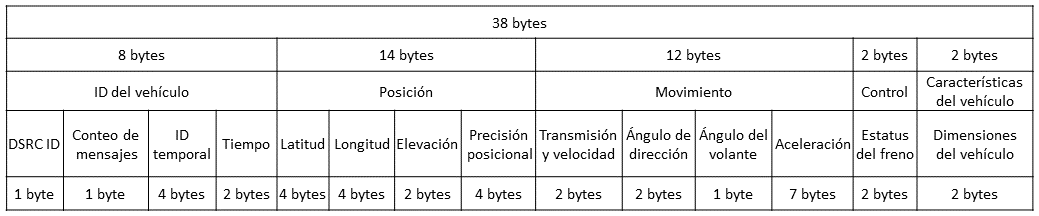
\includegraphics[scale=0.6]{Imagenes/men1}
		\caption{Mensaje propuesto por la SAE}
		\label{fig:men1}
	\end{figure}	
\par Ell mensaje que se propone es una versión más simplificada del mostrado anteriormente, tomando las siguientes consideraciones:

\begin{itemize}
\item Campo de ID del vehículo: debido a que solo se está trabajando con dos vehículos bajo una misma red, no se necesita ningún tipo de identificación por parte de ambos, es por esto que se remueve completamente el campo, a excepción del tiempo, el cual es enviado en segundos.
\item Campo de posición: debido a que el simulador trabaja es con las coordenadas X e Y, se sustituyeron la latitud y la longitud por estas, además al no trabajarse con la elevación, la misma fue eliminada, así como también la precisión posicional.
\item Campo de movimiento: en este campo solo se removió la transmisión, debido a que no es empleada.
\item Control: no posee ningún cambio.
\item Características del vehículo: debido a que los vehículos usados poseen los mismos atributos físicos, se removió este campo, ya que no hay necesidad de enviar datos que ya conocidos por ambos carros.
\end{itemize}
\par Además de estos cambios, debido a que en simulink se trabaja con variables del tipo double, los datos a enviar poseen una longitud de 8 bytes. Así pues, el mensaje empleado puede ser visto en la figura \ref{fig:mem2}.

\begin{figure}[!h]
	\centering
		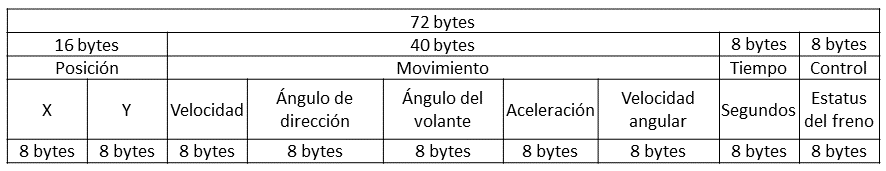
\includegraphics[scale=0.6]{Imagenes/mem2}
		\caption{Mensaje propuesto}
		\label{fig:mem2}
	\end{figure}	  

\section{Implementación en Dynacar}
Como se comentó en secciones anteriores, el sistema de comunicación se programó empleando las S-function, conjunto a la libreria de sockets de Windows, todo esto en los entornos de MATLAB y Simulink. Así pues, se diseñaron tres bloques, uno para enviar la data a otros vehículos, uno para recibir la data de otros vehículos y por último uno para envíar la data del vehículo con el cual que es está realizando la comunicación al Visor 3D de Dynacar. 
\subsection{Módulo de Envío}
Es el módulo encargado de realizar el envío de la data (Figura \ref{fig:send}), posee como entradas:
\begin{itemize}
\item Posición X, Y, ángulo de dirección y velocidad.
\item Ángulo del volante.
\item Tiempo
\item Velocidad angular.
\item Acelerador y Freno.
\end{itemize}

\begin{figure}[!h]
 \centering
  \subfloat[Bloque de envío]{
   \label{fig:a}
    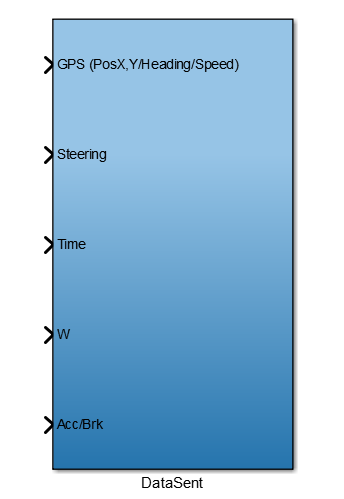
\includegraphics[scale=0.3]{Imagenes/send}}
  \subfloat[Interior del Bloque de envío]{
   \label{fig:v}
    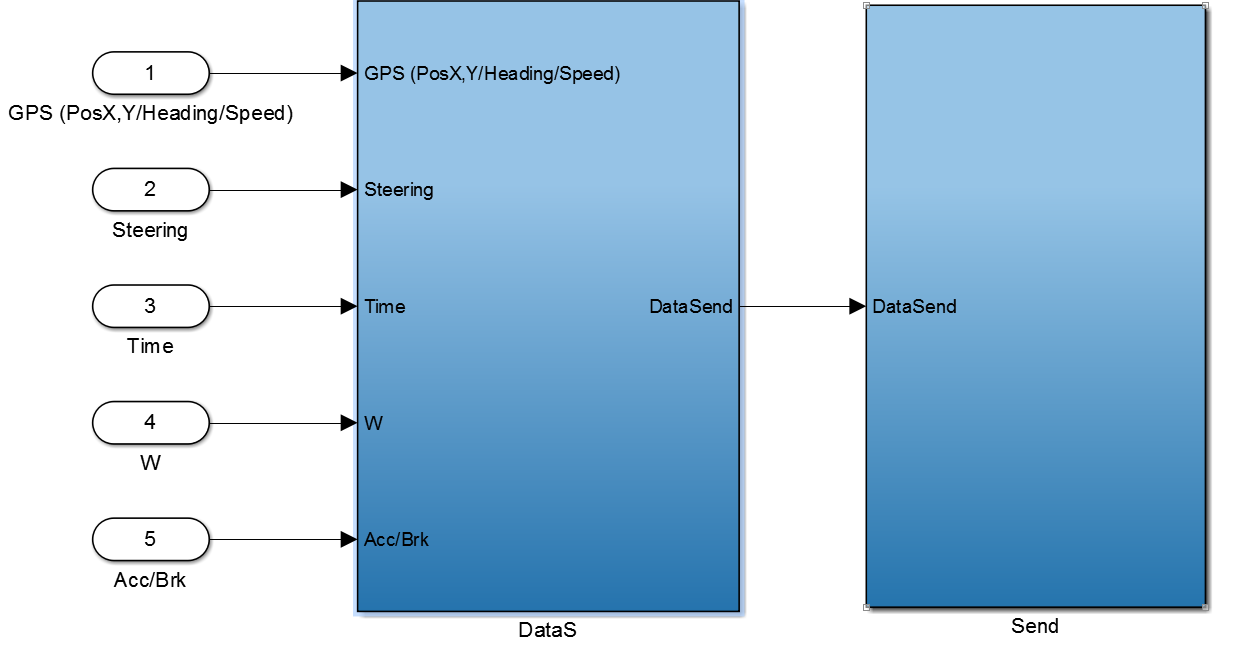
\includegraphics[scale=0.2]{Imagenes/send1}}\\
  \subfloat[Sub-modelo Send]{
   \label{fig:x}
    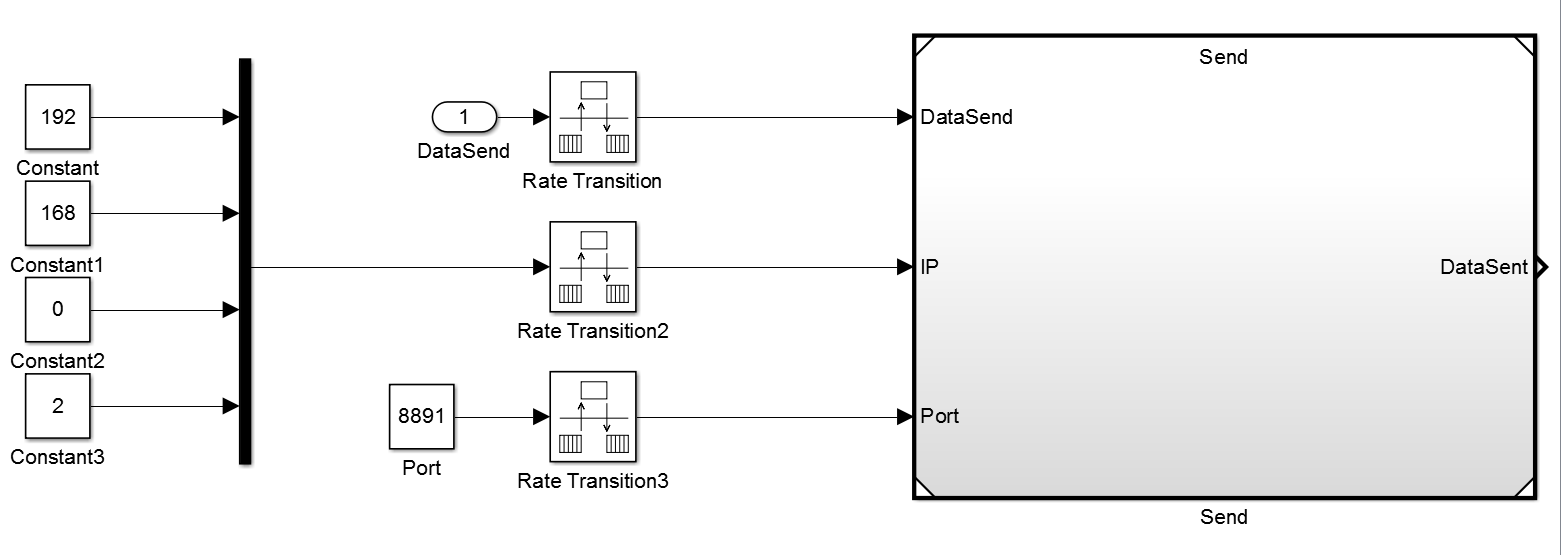
\includegraphics[scale=0.2]{Imagenes/send2}}
 \caption{Estructura del módulo de send}
 \label{fig:send}
\end{figure}

\par Dentro del mismo se encuentra la S-function realizada, que además de recibir los datos a enviar, recibe el IP y el puerto con el cual se va a efectuar la comunicación, datos necesarios para enlazar la computadora con su destino. Una vez activo, dicho bloque siempre estará enviando información, a pesar de que se pueda perder la conexión. Cabe resaltar, que para variar la tasa de envío, se empleó la modalidad de sub-modelos de Simulink, donde en un diagrama principal, se pueden tener bloques secundarios que funcionen a distintos tiempos de muestreo, lo que permite cambiar la tasa, independientemente del esquema principal.          
\subsection{Módulo de Recepción}
Es el bloque encargado de recibir la data proveniente del otro vehículo (Figura \ref{fig:rec}), posee como salidas:

\begin{itemize}
\item Posición X, Y y ángulo de dirección.
\item Velocidad
\item Ángulo del volante.
\item Aceleración.
\item Tiempo.
\item Velocidad angular.
\item Freno.
\end{itemize}

\par Dentro del mismo se encuentra la S-function realizada, que recibe como parámetro, el puerto por el cual se va a obtener la data. Debido a la configuración de los sockets, los mismos están programados para bloquearse hasta recibir información, lo cual perjudica el comportamiento del programa, es por esto que los sockets se configuraron de tal forma que el tiempo de espera sea mayor o igual al tiempo de muestreo del diagrama de simulink, siendo este 1 ms para el simulador y 10 ms para los vehículos. Cabe resaltar, que de la misma forma que para el bloque de envío, se se varía la tasa de recepción a través de un sub-modelo.   

\begin{figure}[!h]
 \centering
  \subfloat[Bloque de recepción]{
   \label{fig:a}
    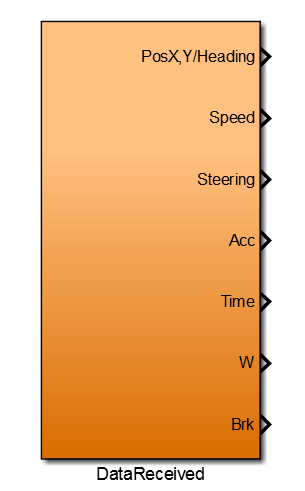
\includegraphics[scale=0.3]{Imagenes/rec2}}
  \subfloat[Interior del Bloque de recepción]{
   \label{fig:v}
    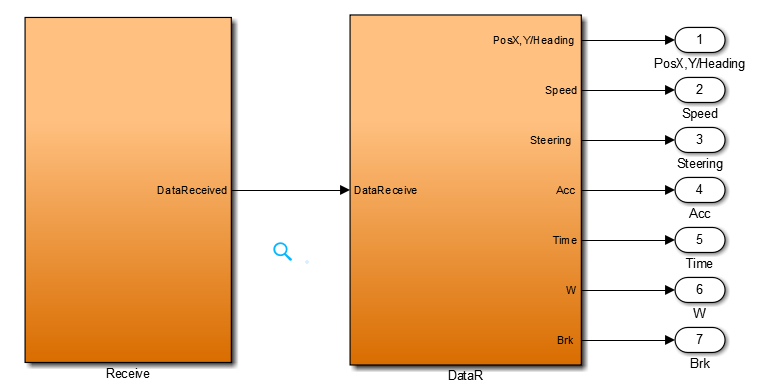
\includegraphics[scale=0.3]{Imagenes/rec1}}\\
  \subfloat[Sub-modelo Receive]{
   \label{fig:x}
    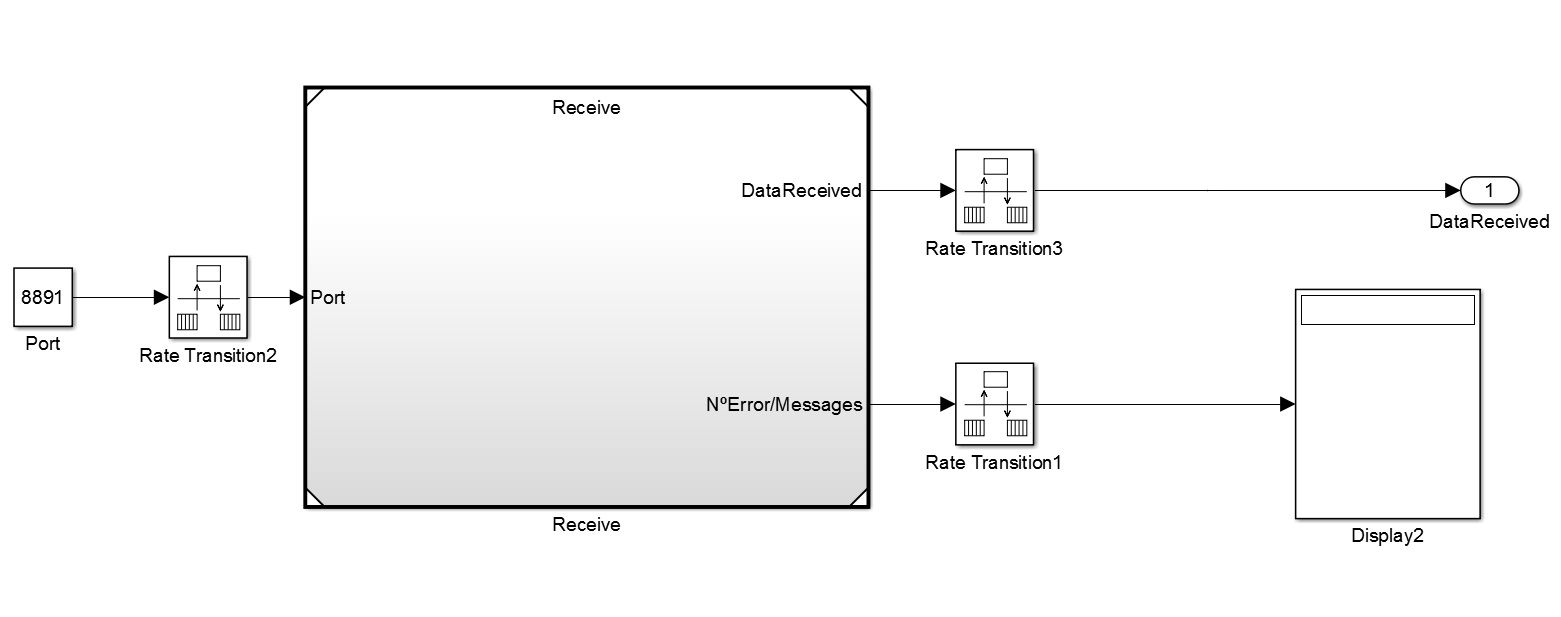
\includegraphics[scale=0.2]{Imagenes/rec3}}
 \caption{Estructura del módulo de recepción}
 \label{fig:rec}
\end{figure}

\subsection{Módulo de Envío al Visor 3D}
Es el módulo encargado de realizar el envío de la data proveniente del vehículo con el cual se está realizando la comunicación (Figura \ref{fig:send}), posee como entradas:

\begin{itemize}
\item Posición X, Y y el ángulo de dirección.
\end{itemize}
\begin{figure}[!h]
 \centering
  \subfloat[Bloque de envío al Visor 3D]{
   \label{fig:a}
    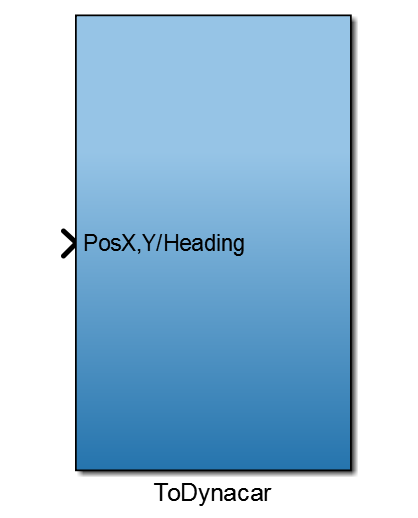
\includegraphics[scale=0.3]{Imagenes/sendtd}}
  \subfloat[Interior del Bloque de envío al Visor 3D]{
   \label{fig:v}
    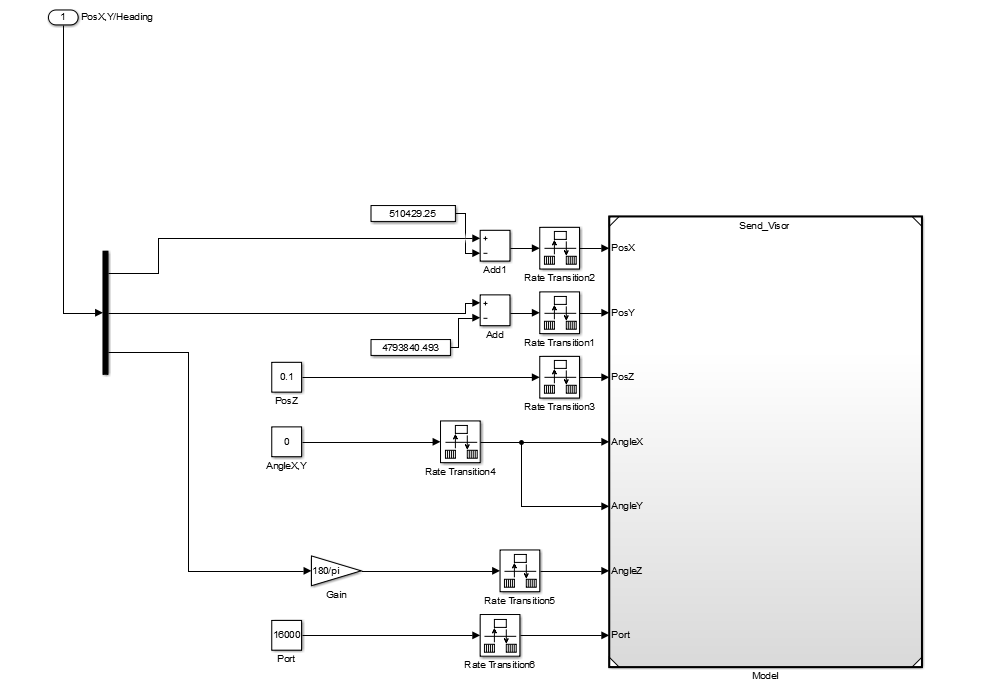
\includegraphics[scale=0.3]{Imagenes/sendtd1}}\\
 \caption{Modelo de envío de información al Visor 3D}
 \label{fig:rec}
\end{figure}

\par Dentro del mismo se encuentra la S-function realizada, que recibe como entrada, el puerto al cual se va a enviar la información, debido a que es una comunicación interna, entre Simulink y el Visor 3D la IP se fija en 127.0.0.1, la cual es empleada cuando se quiere enviar información localmente, o recibir información de cualquier dispositivo. Además el bloque recibe los ángulos con respecto a los otros ejes y la posición en Z, valores que se establecen como 0, debido que no se presenta ningún tipo de movimiento en estos ejes. De la misma forma que para los bloques anterior se realizó un sub-modelo, con el cual se varia la tasa de envío, dicha tasa se fijó en 5 ms para minimizar el coste computacional, y no presentar efectos de retraso con respecto al esquema principal de Dynacar.  

\subsection{Prueba del Sistema de Comunicación a Distintas Tasas de Envío}

Debido a la probablidad de pérdida de paquetes que se puede presentar al utilizar el protocolo UDP, se procede a observar el comportamiento de uno de los módulo que emplee los datos provenientes del vehículo con el cual se está conectado, más específicamente se observa el módulo del ACC, y como responde el controlador ante los mensajes perdidos y las diferentes tasas de envío.\\
 \par Más concretamente, se realizaron 6 pruebas por cada tasa de envío considerada, siendo estas 1 ms, 5 ms, 10 ms, 15, ms 25 ms, 50 ms y 100 ms, de las cuales se reportó la cantidad total de mensajes envíados y mensajes perdidos. Cabe destacar que se este conjunto de pruebas se hicieron tomando en cuenta los efectos que pueda producir el visor 3D.
\subsubsection{Pruebas sin el Visor 3D}  

\begin{itemize}
\item 1 ms
\begin{figure}[H]
	\centering
		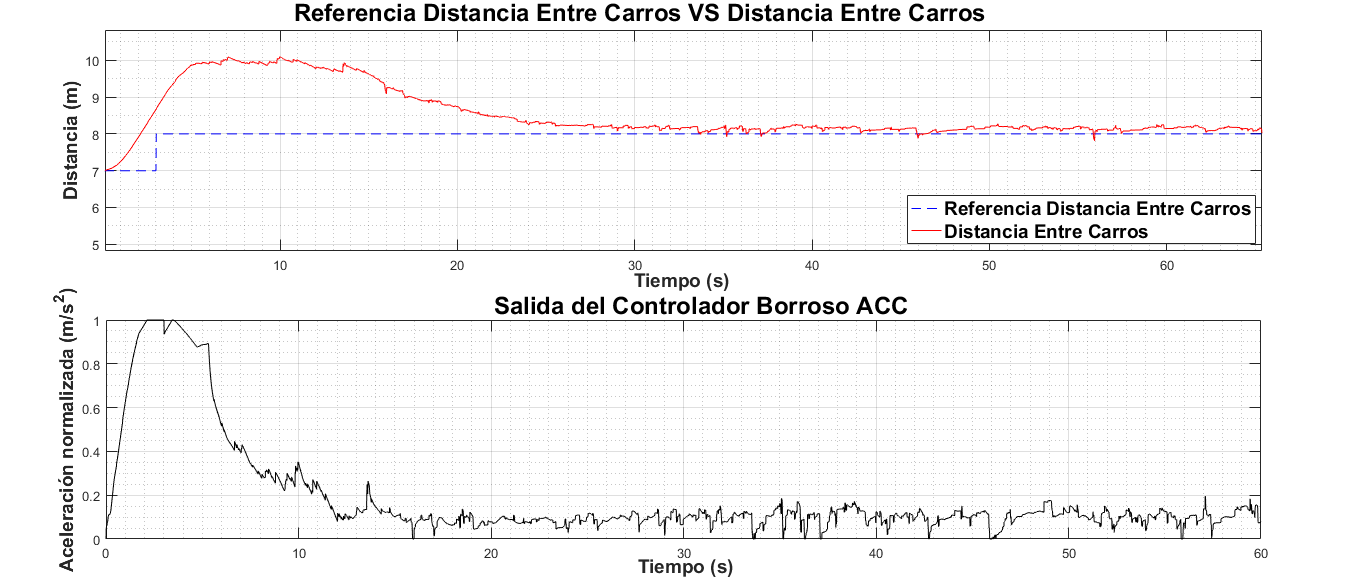
\includegraphics[scale=0.49]{Imagenes/1cv}
		\caption{Gráfica del comportamiento del controlador con una tasa de envío de 1 ms}
		\label{fig:sv1}
\end{figure}
\item 5 ms\\
\begin{figure}[H]
	\centering
		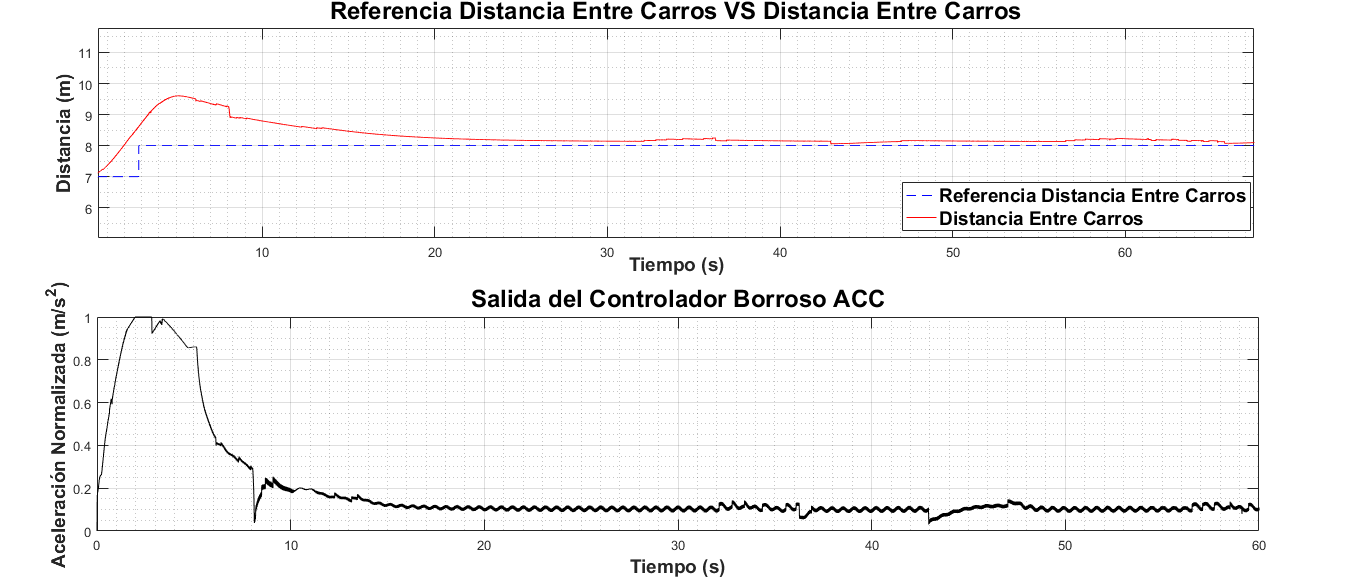
\includegraphics[scale=0.49]{Imagenes/5cv}
		\caption{Gráfica del comportamiento del controlador con una tasa de envío de 5 ms}
		\label{fig:sv5}
\end{figure}	
\item 10 ms
\begin{figure}[H]
	\centering
		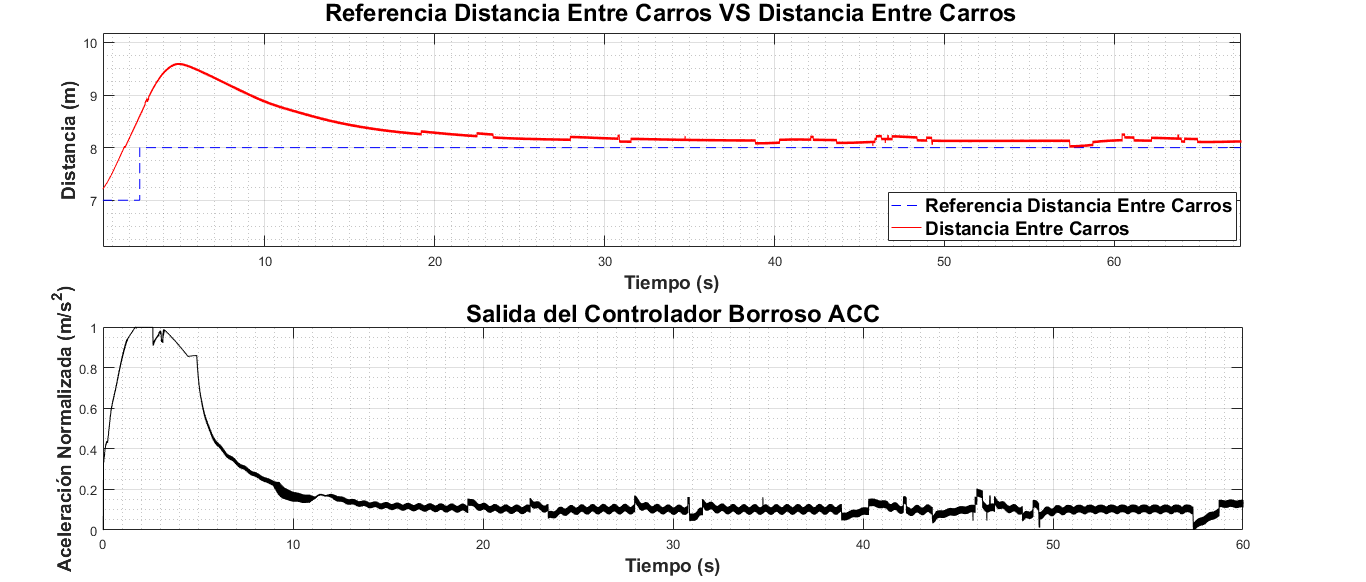
\includegraphics[scale=0.495]{Imagenes/10sv}
		\caption{Gráfica del comportamiento del controlador con una tasa de envío de 10 ms}
		\label{fig:sv10}
\end{figure}	
\item 15 ms
\begin{figure}[H]
	\centering
		\includegraphics[scale=0.49]{Imagenes/15sv}
		\caption{Gráfica del comportamiento del controlador con una tasa de envío de 15 ms}
		\label{fig:sv15}
\end{figure}	
\item 25 ms
\begin{figure}[H]
	\centering
		\includegraphics[scale=0.49]{Imagenes/25sv}
		\caption{Gráfica del comportamiento del controlador con una tasa de envío de 25 ms}
		\label{fig:sv25}
\end{figure}	
\item 50 ms
\begin{figure}[H]
	\centering
		\includegraphics[scale=0.49]{Imagenes/50cv}
		\caption{Gráfica del comportamiento del controlador con una tasa de envío de 50 ms}
		\label{fig:sv50}
\end{figure}	

\item 100 ms
\begin{figure}[H]
	\centering
		\includegraphics[scale=0.49]{Imagenes/100cv}
		\caption{Gráfica del comportamiento del controlador con una tasa de envío de 100 ms}
		\label{fig:sv100}
\end{figure}	  	  
\end{itemize}

\par Observando las figuras \ref{fig:sv1}, \ref{fig:sv5}, \ref{fig:sv10}, \ref{fig:sv15}, \ref{fig:sv25}, \ref{fig:sv50}, \ref{fig:sv100} se puede apreciar que a medida que se aumenta la tasa de envío, aumenta el ruido en el controlador, lo cual es producto de la diferencia entre el procesamiento de data a 1 ms del esquema principal del simulador, con la proveniente del bloque de recepción. Con el fin de contrastar de  mejor forma este efecto, se realizó un acercamiento a las figuras \ref{fig:sv5} y \ref{fig:sv50}, siendo este mostrado en la imagen \ref{fig:comp}:   

\begin{figure}[H]
 \centering
  \subfloat[Acercamiento de la figura \ref{fig:sv5}]{
   \label{fig:cinco}
    \includegraphics[scale=0.22]{Imagenes/zoom5}}
  \subfloat[Acercamiento de la figura \ref{fig:sv50}]{
   \label{fig:cincuenta}
    \includegraphics[scale=0.23]{Imagenes/zoom50}}\\
 \caption{Comparación entre la figuras \ref{fig:sv5} y la figura \ref{fig:sv50}}
 \label{fig:comp}
\end{figure}

\par Se puede observar en la figura \ref{fig:cinco} que efectivamente se tiene un período de 5 ms, que corresponde a la tasa de envío establecida, la cual produce una variación a la salida del controlador al estabilizarce de $ \pm 0.015$, lo que equivale a una acción del 1.5 \% sobre los actuadores, valor que posteriormente, por como están configurados el freno y el acelerador se divide a la mitad, teniendo así, un valor final del 0.75 \%, acción que puede ser considerada como despreciable. A diferencia, da la figura \ref{fig:cincuenta}, en la cual se presenta un período de 50 ms, que genera una variación de $ \pm 10 \% $, que se traduce al final en un 5 \%, dicho valor se puede ver aumentado hasta un 25 \% cuando se pierde un paquete. \\  

\par A continuación se presenta la tabla \ref{tab:tabcv}, donde se presenta la relación de menseajes totales, con mensajes perdidos. En la misma se observa que a medida de que aumenta la tasa de envío se reduce la cantidad de mensajes perdidos, así como la probabilidad de ocurrencia. De las tasas probadas se destaca la de 1 ms, la cual presenta la mayor cantidad de mensajes perdidos, efecto que se debe, a que el número de procesos manejados por el simulador al mismo tiempo, afecta de manera negativa el rendimiento de la PC, interfierendo con la recepción de data. Esto produce que se exceda con mayor frecuencia el tiempo de espera establecido sin recibir ningún paquete y de esta forma se perjudican los módulos que hacen uso de estos datos, como es apreciado en la figura \ref{fig:sv1}, donde la señal del error de la distancia tarda más tiempo (28 s) en apegarse a la referencia, a diferencia de las demás tasas (20 s). \\

\begin{table}[htbp]
  \centering
\resizebox{\textwidth}{!}{
% Table generated by Excel2LaTeX from sheet 'Hoja1'
  \begin{tabular}{|l|l|l|l|}
    \toprule
    \multicolumn{1}{|p{9.43em}|}{Tiempo de envío (ms)} & \multicolumn{1}{p{10.5em}|}{Cantidad de mensajes} & \multicolumn{1}{p{10.07em}|}{Mensajes perdidos} & \multicolumn{1}{p{8.785em}|}{\% De mensajes perdidos} \\
    \midrule
    1     & 81457 & 1909  & 2,34 \\ 
    \midrule
    5     & 16258 & 62    & 0,38 \\ 
    \midrule
    10    & 8154  & 45    & 0,55 \\ 
    \midrule
    15    & 5435  & 15    & 0,27 \\ 
    \midrule
    25    & 3260  & 13    & 0,41 \\ 
    \midrule
    50    & 1648  & 7     & 0,45 \\ 
    \midrule
    100   & 813   & 1     & 0,18 \\ 
    \bottomrule
    \end{tabular}}%
  \caption{Prueba del sistema de comunicación a distintas tasas de envío sin emplear el Visor 3D}
  \label{tab:tabsv}%
\end{table} %

\par Tomando en cuenta los resultados arrojados por las pruebas realizadas, se elijió como tasa de envío, 5 ms, ya que es la que presenta menos delay, y si bien, posee mayor perdida de paquetes que las demás tasas, no se ve afectada fuertemente, a diferencia de por ejemplo la de 25 ms, que puede generar a la salida del controlador una señal errada de más del 20 \%, tras un paquete perdido. Además, como no coincide con el tiempo de muestreo del simulador, se reducen los efectos del rendimiento del computador sobre la recepción de paquetes, mostrando así, un comportamiento más que aceptable, teniendo en cuenta las dificultadas presentadas.         

\subsubsection{Pruebas con el Visor 3D}  

A continuación, al igual que en el punto anterior, se pueden observar las gráficas del comportamiento del controlador ante las tasas de envío de 1 ms, 5 ms, 10 ms, 15 ms, 25 ms, 50 y 100 ms, pero esta vez usando el Visor 3D, el cual, además de aumentar la cantidad de procesos que tiene que ejectutar la computadora, se comunica con Simulink mediante sockets de UDP, lo que genera un mayor tráfico de paquetes, aumentando la probabilidad de que se pueda perder un paquete.   

\begin{itemize}
\item 1 ms
\begin{figure}[H]
	\centering
		\includegraphics[scale=0.5]{Imagenes/1sv}
		\caption{Gráfica del comportamiento del controlador con una tasa de envío de 1 ms}
		\label{fig:cv1}
\end{figure}
\item 5 ms
\begin{figure}[H]
	\centering
		\includegraphics[scale=0.48]{Imagenes/5sv}
		\caption{Gráfica del comportamiento del controlador con una tasa de envío de 5 ms}
		\label{fig:cv5}
\end{figure}	
\item 10 ms
\begin{figure}[H]
	\centering
		\includegraphics[scale=0.49]{Imagenes/10cv}
		\caption{Gráfica del comportamiento del controlador con una tasa de envío de 10 ms}
		\label{fig:cv10}
\end{figure}	
\item 15 ms
\begin{figure}[H]
	\centering
		\includegraphics[scale=0.48]{Imagenes/15cv}
		\caption{Gráfica del comportamiento del controlador con una tasa de envío de 15 ms}
		\label{fig:cv15}
\end{figure}	
\item 25 ms
\begin{figure}[H]
	\centering
		\includegraphics[scale=0.49]{Imagenes/25cv}
		\caption{Gráfica del comportamiento del controlador con una tasa de envío de 25 ms}
		\label{fig:cv25}
\end{figure}	
\item 50 ms
\begin{figure}[H]
	\centering
		\includegraphics[scale=0.48]{Imagenes/50sv}
		\caption{Gráfica del comportamiento del controlador con una tasa de envío de 50 ms}
		\label{fig:cv50}
\end{figure}	
\item 100 ms
\begin{figure}[H]
	\centering
		\includegraphics[scale=0.47]{Imagenes/100sv}
		\caption{Gráfica del comportamiento del controlador con una tasa de envío de 100 ms}
		\label{fig:cv100}
\end{figure}	  	  
\end{itemize}

\par Observando las figuras \ref{fig:cv1}, \ref{fig:cv5}, \ref{fig:cv10}, \ref{fig:cv15}, \ref{fig:cv25}, \ref{fig:cv50}, \ref{fig:cv100} se puede apreciar que empeoran su comportamiento con respecto a las pruebas hechas sin el visor 3D, sobre todo con la tasa de 1 ms, la cual no llega ni a apegarse a la referencia. Sin embargo la señal de la distancia si logra alcanzar la referencia, con el mismo tiempo (20 s), con las demás tasas, viendo empeorado, de esta forma solo el comportamiento del controlador, haciéndolo más suseptible ante un paquete perdido.\\      

\par De la misma forma se reportaron las estadíticas relacionadas a la cantidad de mensajes perdidos, datos que pueden ser apreciados en la tabla \ref{tab:tabcv}. 

\begin{table}[htbp]
  \centering
\resizebox{\textwidth}{!}{
% Table generated by Excel2LaTeX from sheet 'Hoja1'
    \begin{tabular}{|c|c|c|c|}
    \toprule
    \multicolumn{1}{|p{9.43em}|}{Tiempo de envío (ms)} & \multicolumn{1}{p{10.5em}|}{Cantidad de mensajes} & \multicolumn{1}{p{10.07em}|}{Mensajes perdidos} & \multicolumn{1}{p{8.785em}|}{\% De mensajes perdidos} \\
    \midrule
    1     & 81457 & 14124 & 17,34 \\
    \midrule
    5     & 16258 & 272   & 1,67 \\
    \midrule
    10    & 8154  & 132   & 1,62 \\
    \midrule
    15    & 5435  & 89    & 1,64 \\
    \midrule
    25    & 3260  & 54    & 1,64 \\
    \midrule
    50    & 1648  & 27    & 1,66 \\
    \midrule
    100   & 813   & 3     & 0,33 \\
    \bottomrule
    \end{tabular}}%
  \caption{Prueba del sistema de comunicación a distintas tasas de envío empleando el Visor 3D}
  \label{tab:tabcv}%
\end{table}%

\par De los datos obtenidos de la tabla \ref{tab:tabcv} se puede contemplar que la pérdida de paquetes es 4 veces mayor, que cuando no se usa el visor, a excepción de las tasas de 1 ms y 100 ms, siendo iguales para la útltima y 8 veces mayor para la primera, valor muy elevado, que, como se observa en la figura \ref{fig:cv1}, evita que se pueda cumplir el objetivo del controlador. Si bien la pérdida de paquetes aumentó en gran medida con respecto a las pruebas anteriores, estas probabilidades son menores al 2 \%, lo cual aún no genera un impacto lo suficientemente negativo como para no emplear alguna de estas tasas. Por lo que de la misma forma se elijío como tasa de envío la de 5 ms, ya que es la que muestra la mejor respuesta, en comparación con las demás. \\ 

\par Finalmente, se probó un último escenario, en donde la comunicación se realiza en una sola dirección, es decir un vehículo solo envía información, mientras que el otro solo recibe. Dicho escenario es el presentado en los Twizys, donde uno solo envía información (semi-automatizado), y el otro la recibe (completamente automatizado), siendo este último el encargado de realizar las maniobras. \\  

\par Para esta prueba solo se observó el comportamiento con una tasa de 1 ms, debido a que es el tiempo de muestreo del simulador, siendo 10 ms el equivalente de los vehículos. El resultado puede ser visto en la figura \ref{fig:sr}, donde en promedio, se tuvieron 361 mensajes perdidos de 81457 mensajes, representando de esta forma el 0.44 \%, disminuyendo considerablemente la cantidad de paquetes perdidos con respecto a las pruebas de las comunicaciones bidireccionales. Dicho esto se considera factible emplear una tasa de envío igual al tiempo de muestro del simulador cuando se presenta un escenario de comunicación unidireccional. 
\
\begin{figure}[H]
	\centering
		\includegraphics[scale=0.4]{Imagenes/1svc}
		\caption{Gráfica del comportamiento del controlador con una tasa de envío de 1 ms}
		\label{fig:sr}
\end{figure}	  	  

\section{Resumen}
En el capítulo 5 se presentó el sistema de comunicación implementado, argumentando el uso de dispositivos comerciales, para lo cual se realizó una exhaustiva comparación entre los protocolos de las WLAN y las VANET's. De dicha comparación se obtuvo que bajo circunstancias de bajo tráfico, donde los vehículos están ya conectados en una misma red, y se envían mensajes periódicos el sistema de comunicación comercial puede emular al vehicular.\\
\par Posteriormente, se realizó una comparación entre los protocolos de transporte UDP y TCP, que arrojó como resultado, que el más idonio es el protocolo UDP, ya que por su velocidad de transporte y no necesitar un enlace de conección fijo, puede cumplir con los requerimientos de las comunicaciones vehiculares. Luego se planteó el mensaje a usar, el cual está basado en el propuesto por la SAE.\\
\par Finalmente, se describió los bloques que conforman el sistema de comunicación implementados en Dynacar, para después observar la respuesta del sistema ante distintas tasas de envío, y las pérdidas de paquetes. De dichas pruebas se obtuvo que para ambos casos, con el Visor 3D y  sin el Visor 3D, la mejor tasa de envío es la de 5 ms, y en el caso de emplear comunicaciones unidireccionales es viable emplear una tasa igual al tiempo de muestreo del simulador, siendo 1 ms para Dynacar y 10 ms para los vehículos.      
%%Resultados experimentales
\chapter{Maniobras Cooperativas}\label{sec:capitulo6}
\thispagestyle{empty}

En el presente capítulo se describen las maniobras coperativas realizadas, ACC, Control Lateral, \textit{Stop and Go} y ACC con Control Lateral. Explicando para las dos primeras maiobras, el algoritmo de control realizado, así como su implementación en Dynacar, ambos basados en la lógica difusa.\\

\par Posteriormente se describen las pruebas realizadas, así como sus resultados, teniendo para el ACC y el \textit{Stop and Go}, pruebas de desempeño a bajas y medias velocidades, y para el Control Lateral, tanto con el ACC, como sin el mismo, pruebas con distintos tipos de curvas, más específicamente las presentadas en el escenerio de TECNALIA \textit{Research \& Innovation}.  


\section{ACC Longitudinal}
Como se expuso anteriormente , esta maniobra busca mantener la velocidad del vehículo, tomando en cuenta la velocidad del carro que tiene al frente, así como guardar cierta distancia con respecto al mismo. Para conseguir esto, se realizó un controlador difuso\cite{perez2013cooperative} que recibe como entradas los errores de velocidad y de distancia, y como salida, las respectivas acciones sobre los actuadores.  

\subsection{Algoritmo de Control}

Para comprender mejor las consideraciones empleadas para desarrollar el algoritmo, se presenta la Figura \ref{fig:acce}, en donde, se tienen tres distancias, $ D_{L-S}$, $ D_{S}$ y D. Siendo $D_{L-S}$ la distancia actual entre los vehículos, $D_{S}$ la distancia de seguridad establecida, que a efectos del presente trabajo posee un valor de 7 m, y finalmente D, la distancia ideal a la cual deberían de estar los vehículos.\\

\begin{figure}[!h]
	\centering
		\includegraphics[scale=0.5]{Imagenes/acce}
		\caption{Caractrísticas del ACC implementado}
		\label{fig:acce}
	\end{figure}	 

\par Entonces, teniendo en cuenta que se trabaja con la velocidad y la posción X y Y, de los vehículos, los errores son calculados de la siguiente forma:

\begin{itemize}
\item Error de Velocidad: para el cálculo del error de velocidad, basta con solo la resta de las mismas.
\begin{equation} \label{eq: errvel}
E_{Vel} = V_{L} - V_{S}
\end{equation}
\par Error, que si resulta positivo, quiere decir que la velocidad del vehículo líder es mayor a la del seguidor, por ende el carro seguidor deberá acelerar, mientras que si es negativo la velocidad del vehículo seguidor es mayor a la del líder, por lo que el carro deberá frenar. Siempre y cuando la distancia entre los vehículos no sea muy grande, caso en el cual el vehículo seguidor deberá acelerar para alcanzarlo sin importar la velocidad del vahículo líder.
\item Error de Distancia: para calcular este error se restan los valores de $D_{L-S}$ y D, los cuales se obtienen de la siguiente forma:
\begin{itemize}
\item Distancia entre vehículos: como se poseen son los valores de la posciión X, Y de los carros, se procede a buscar la distancia entre dos puntos.
\begin{equation} \label{eq: distv}
D_{L-S} = \sqrt{(X_{L}-X_{S})^{2} + (Y_{L}-Y_{S})^{2}}
\end{equation}

\item Distancia de referencia: para calcular esta distancia, se hizo uso de la fórmula del cuadrado de la velocidad, dada por la dirección general de tráfico española, DGT \footnote{http://www.dgt.es/es/seguridad-vial/}, a la cual por razones de seguridad se le añadieron 7 m más, que corresponden a la distancia de seguridad. 

\begin{equation} \label{eq: diss}
D = (Entero(\frac{V_{S}}{10}))^{2} + D_{S}
\end{equation}

\end{itemize}
\par Con lo cual error de la distancia resulta:
\begin{equation} \label{eq: errvel}
E_{Dist} = D_{L-S} - D
\end{equation}

\par Valor que si da positivo quiere decir que se supera la distancia de referencia, implicando que el vehículo deberá de acelerar, mientras que si es negativo, la distancia entre los vehículos es menor que la de referencia, por lo que el carro tendrá que frenar.

\end{itemize} 
\subsection{Implementación en el Simulador}

Para la implementación en Dynacar de este controlador se hizo uso del ToolBox de MATLAB para controladores difusos, al cual se le pasan como entradas las variables medidas, que en este caso son el error de la velocidad y el error de la distancia, y como salida las variables a controlar, acelerador y freno (Figura \ref{fig:accdyna})\\ 

\begin{figure}[!h]
	\centering
		\includegraphics[scale=0.3]{Imagenes/accdyna}
		\caption{Implementación del ACC en Simulink}
		\label{fig:accdyna}
\end{figure}	 

\par Dentro del ToolBox se configuran las funciones de pertenencia, tanto de las entradas (Figuras \ref{fig:fuzzyvel} y \ref{fig:fuzzydist}), como de las salidas (Figura \ref{fig:fuzzyacc}), así como tambien las reglas planteadas. Cada elemento corresponde a un bloque del esquema que rige a los controladores difusos, siendo estos el de fuzzficación, defuzzyficación e inferencia, respectivamente, acotando que, como método de inferencia se empleó el de Mamdani y de defuzzyficación el del centroide, métodos establecidos como predeterminados en el ToolBox. 

\begin{itemize}

\item Función de Pertenencia del Error de Velocidad: para este parámetro se fijaron cuatro funciones, muy negativo, negativo, central y positivo, con el fin de ajustar de mejor forma la velocidad del vehículo, cuando este se encuentre cerca del valor de referencia. Además se adecuó el rango, de forma que no fuese muy amplio para tener un mejor control a velocidades bajas y medias. 

\begin{figure}[!h]
	\centering
		\includegraphics[scale=0.35]{Imagenes/fuzzyvel}
		\caption{Función de pertenencia del Error de Velocidad}
		\label{fig:fuzzyvel}
\end{figure}	 

\item Función de Pertenencia del Error de Distancia: para este parámetro de fijaron cuatro funciones, negativo, central, positivo y muy positivo, con el fin de ajustar la relación de distancia, de la misma forma que en el error de la velocidad para mantener el error cerca de la referencia, sin cambios bruscos.

\begin{figure}[!h]
	\centering
		\includegraphics[scale=0.35]{Imagenes/fuzzydist}
		\caption{Función de pertenencia del Error de Distancia}
		\label{fig:fuzzydist}
\end{figure}	 

\end{itemize}
   
\par Dichos parámetros se seleccionaron utilizando la lógica experimental, observando los resultados obtenidos previamente y analizando la manera en que el controlador debería modificar la referencia de velocidad y distancia, según sea el escenario para lograr el objetivo planteado. Las reglas se constituyen de la siguiente forma:\\

	\hspace*{2pt}IF ErrorVel $Negativo$ AND ErrorDist $Positivo$ THEN ACC/BRK $NADA$\\
	\hspace*{20pt}IF ErrorVel $Negativo$ AND ErrorDist $Central$ THEN ACC/BRK $BRK$\\
	\hspace*{20pt}IF ErrorVel $Negativo$ AND ErrorDist $Negativo$ THEN ACC/BRK $BRKH$\\
	\hspace*{20pt}IF ErrorVel $Nada$ AND ErrorDist $Negativo$ THEN ACC/BRK $BRK$\\
	\hspace*{20pt}IF ErrorVel $Nada$ AND ErrorDist $Nada$ THEN ACC/BRK $NADA$\\
	\hspace*{20pt}IF ErrorVel $Nada$ AND ErrorDist $Positivo$ THEN ACC/BRK $ACC$\\
	\hspace*{20pt}IF ErrorVel $Positivo$ AND ErrorDist $Negativo$ THEN ACC/BRK $NADA$\\
	\hspace*{20pt}IF ErrorVel $Positivo$ AND ErrorDist $Nada$ THEN ACC/BRK $ACC$\\
	\hspace*{20pt}IF ErrorVel $Positivo$ AND ErrorDist $Positivo$ THEN ACC/BRK $ACCH$\\
	\hspace*{20pt}IF ErrorVel $MuyNegativo$ THEN ACC/BRK $BRKH$\\
	\hspace*{20pt}IF ErrorDist $MuyPositivo$ THEN ACC/BRK $ACCH$\\

\par En el caso de la salida, la misma esta contituida por 5 valores del tipo \textit{singleton} dentro del conjunto $\in$ [-1;1], donde los valores negativos corresponden al freno, y los positivos al acelerador. De la misma forma que para las entradas, los valores de salida se definieron de manera experimental, observando los resultados a medida que se modificaban los valores progresivamente.\\

\begin{figure}[!h]
	\centering
		\includegraphics[scale=0.30]{Imagenes/fuzzyacc}
		\caption{Función de pertenencia de la Salida del Controlador}
		\label{fig:fuzzyacc}
\end{figure}	 

\par La configuración completa de las salidas, junto a las funciones de pertenencia y a las reglas dan como resultado la siguiente superficie de control (Figura \ref{fig:supacc}), mediante la cual se puede predecir el comportamiento exacto del controlador a partir de ambas entradas.\\

\begin{figure}[!h]
	\centering
		\includegraphics[scale=0.4]{Imagenes/supacc}
		\caption{Superficie de control generada}
		\label{fig:supacc}
\end{figure}	 

\subsection{Pruebas en Dynacar a Distintas Velocidades}

Para las pruebas de este controlador se emplearon dos módulos de Dynacar en un mismo diagrama de Simulink (Figura \ref{fig:dyna2}), con el cual se simulan dos vehículos en una misma computadora, ignorando los efectos que pueda introducir el módulo de comunicación, y de esta forma analizar con más certeza el desempeño del controlador. 

\begin{figure}[!h]
	\centering
		\includegraphics[scale=0.30]{Imagenes/dyna2}
		\caption{Diagrama de Simulink con dos módulos de Dynacar}
		\label{fig:dyna2}
\end{figure}	 

\par Así pues, se devidió las pruebas según la velocidad propuesta, siendo estas, velocidades bajas y velocidades medias.
%%%%%%%%%%%%%%%%%%%%%%%
\subsubsection{Velocidades Bajas}
%%%%%%%%%%%%%%%%%%%%%%%
En las Figuras \ref{fig:velvb} y \ref{fig:distvb} se puede encontrar el comportamiento del controlador a velocidades bajas, las cuales son establecidas en el rango de 10 Km/h a 30 Km/h. Más específicamente se observan las velocidades de los vehículos y la distancia entre los mismos.\\

\begin{figure}[H]
	\centering
		\includegraphics[scale=0.35]{Imagenes/accvb}
		\caption{Gráfica de la velocidad de los vehículos}
		\label{fig:velvb}
\end{figure}	

\begin{figure}[H]
	\centering
		\includegraphics[scale=0.35]{Imagenes/accvmdist}
		\caption{Gráfica del error de la distancia de los vehículos}
		\label{fig:distvb}
\end{figure}	

\par Observando la Figura \ref{fig:velvb} se puede apreciar que tanto a 10 Km/h, como a 20 Km/h el vehículo seguidor se apega correctamente a la velocidad del líder, mostrando un error de 2 Km/h, al realizar el cambio de velocidad, mientras que en el cambio a 30 Km/h se presenta un error mayor, de 4 Km/h, el cual sigue siendo aceptable, logrando corregirse en un tiempo de 5 s. En lo que respecta a la distancia, la Figura \ref{fig:distvb}, muestra que el error máximo que se presenta es de 50 cm, con respecto a la referencia, y que tarda 10 s, en alcanzar dicho valor.

%%%%%%%%%%%%%%%%%%%%%%%
\subsubsection{Velocidades Medias}
%%%%%%%%%%%%%%%%%%%%%%%

En las Figuras \ref{fig:velvm} y \ref{fig:distvm} se puede encontrar el comportamiento del controlador a velocidades medias, las cuales son establecidas en el rango de 40 Km/h a 60 Km/h. De igual forma, se observan las velocidades de los vehículos y la distancia entre los mismos.

\begin{figure}[H]
	\centering
		\includegraphics[scale=0.35]{Imagenes/accvm}
		\caption{Gráfica de la velocidad de los vehículos}
		\label{fig:velvm}
\end{figure}	

\begin{figure}[H]
	\centering
		\includegraphics[scale=0.35]{Imagenes/accvbdist}
		\caption{Gráfica del error de la distancia de los vehículos}
		\label{fig:distvm}
\end{figure}	

\par En lo que respecta a la Figura \ref{fig:velvm} se puede apreciar que los errores al alcanzar la referencia aumentan, resultando en 0.5 Km/h por debajo de la velocidad del vehículo líder, siendo esto un error equivalente al 1 \%, mientras que para alcanzar el valor de rerencia se manetiene el error de 2 Km/h. El tiempo de establecimiento es de 14 s, 4 segundos más que el que tarda para estabilizarce en las velocidades bajas 


%%%%%%%%%%%%%%%%%%%%%%%%%%%%%%%%%%%%%%%%%
\section{Control Lateral}
%%%%%%%%%%%%%%%%%%%%%%%%%%%%%%%%%%%%%%%%%
Esta maniobra busca mantener la posición y dirección, tomando en cuenta la posición del carro que tiene al frente. Para conseguir esto, se realizó un controlador difuso\cite{sriranjanlateral} que recibe como entradas el error lateral y el error angular, y como salida, el ángulo que debe mantener el volante.  

\subsection{Algoritmo de Control}

Para el cálculo de los errores se emplea la posición del vehículo líder, con la cual se arma un vector de 150 valores, que se actualiza cada 50 ms, donde además, se guarda la dirección del vehículo en dichos puntos. Con estos valores se compara la posición y dirección del vehículo seguidor, pudiendo así obtener el error lateral y angular (Figura \ref{fig:cle}). 


\begin{figure}[!h]
	\centering
		\includegraphics[scale=0.40]{Imagenes/cle}
		\caption{Caractrísticas del Control Lateral implementado}
		\label{fig:cle}
	\end{figure}	 

Entonces, proyectando la posición del vehículo la posción a las ruedas delanteras, se tiene que los errores son calculados de la siguiente forma:

\begin{itemize}

\item Error Lateral: para el cálculo del error lateral se toma en cuenta, que el mismo es la distancia que existe entre el punto de control delantero hasta el segemento de recta en el cual se encuentra el vehículo. Con esto dicho, se busca un punto de esta recta que se ecnuentre más cerca a la pocisión del vehículo y se calcula el error, con la siguiente fórmula: 

\par Proyección de la posición del vahículo al punto de control delantero (\textit{Lookahead}):

\begin{equation} \label{eq:distel}
X = Lookahead\cdot \cos({\textit{heading}})
\end{equation}
\begin{equation} \label{eq:distel}
Y = Lookahead\cdot \sen({\textit{heading}})
\end{equation}
\par Error lateral:
\begin{equation} \label{eq:distel}
E_{Lat} = \sqrt{(X_{VS}-X_{Seg})^{2} + (Y_{VS}-Y_{Seg})^{2}}
\end{equation}

\par Para saber la orientación del error, se calcula el producto escalar, de los vectores formados por la posición del vehículo y el segmento de recta, valor, que sí resulta positivo, quiere decir que el vehículo se encuentra a la derecha de la recta, mientras que si es negativo, se encuentra a la izquierda.

\item Error Angular: para el cálculo de este error, se toma en consideración, que el mismo es las desviación del ángulo del vehículo, con respecto al segmento, el cual puede tomar valores entre [-$\pi$;$\pi$], así pues, el error se calcula el error de la siguiente forma:

\begin{equation} \label{eq:distang}
E_{Ang} = \arctan{\frac{\sen{\psi_{VS}}}{\cos{\psi_{VS}}}} - \arctan{\frac{\sen{\psi_{VL}}}{\cos{\psi_{VL}}}}
\end{equation}
 
\par Valor que si resulta positivo indica que la dirección del vehículo está a la derecha con respecto a la del segmento, mientras que si es negativo se encuentra direccionado a la izquierda. 
\end{itemize}

\subsection{Implementación en el Simulador}

Para la implementación en Dynacar también se hizo uso del ToolBox de Matlab para controladores difusos, al cual se le pasa como entradas el error lateral y el error angular, y tiene como salida el ángulo del volante (Figura \ref{fig:cldyna})


\begin{figure}[!h]
	\centering
		\includegraphics[scale=0.3]{Imagenes/cldyna}
		\caption{Implementación del Control Lateral en Simulink}
		\label{fig:cldyna}
\end{figure}	 

\par De la misma forma se configuraron las funciones de pertenencia de entrada (Figuras \ref{fig:fuzzylat} y \ref{fig:fuzzyang}) y de salida (Figura \ref{fig:clsal}), así como las reglas planteadas, además de emplear el método de inferencia y de desfuzzyficación que el controlador del ACC.

\begin{itemize} 

\item Función de pertenencia del Error Lateral: para este parámetro se fijaron tres funciones, negativo, central y positivo, con una apertura central grande para no mantener el vehículo lo más centrado posible, sin generar cambios bruscos.

\begin{figure}[!h]
	\centering
		\includegraphics[scale=0.29]{Imagenes/fuzzylat}
		\caption{Función de pertenencia del Error Lateral}
		\label{fig:fuzzylat}
\end{figure}	 



\item Función de pertenencia del Error Angular: para este parámetro se fijaron tres funciones, negativo, central y positivo, con una apertura central grande para no mantener la dirección del vehículo lo más cercana posible a la del vehículo líder, sin generar cambios abruptos.

\begin{figure}[!h]
	\centering
		\includegraphics[scale=0.29]{Imagenes/fuzzyang}
		\caption{Función de pertenencia del Error Angular}
		\label{fig:fuzzyang}
\end{figure}	 
\end{itemize}

\par Al igual que con el controlador del ACC, estos parámetros fueron seleccionados utiliando la lógica experimental, observando su comportamiento y ajustándolo según sea necesario. Las reglas planteadas son las siguientes:\\

	\hspace*{2pt}IF ErrorAng $Negativo$ AND ErrorDist $Negativo$ THEN Steering $HIzquierda$\\
	\hspace*{20pt}IF ErrorAng $Negativo$ AND ErrorDist $Central$ THEN Steering $MIzquierda$\\
	\hspace*{20pt}IF ErrorAng $Negativo$ AND ErrorDist $Positivo$ THEN Steering $Izquierda$\\
	\hspace*{20pt}IF ErrorAng $Central$ AND ErrorDist $Negativo$ THEN Steering $LIzquierda$\\
	\hspace*{20pt}IF ErrorAng $Central$ AND ErrorDist $Central$ THEN Steering $Central$\\
	\hspace*{20pt}IF ErrorAng $Central$ AND ErrorDist $Positivo$ THEN Steering $LDerecha$\\
	\hspace*{20pt}IF ErrorAng $Positivo$ AND ErrorDist $Negativo$ THEN Steering $Derecha$\\
	\hspace*{20pt}IF ErrorAng $Positivo$ AND ErrorDist $Central$ THEN Steering $MDerecha$\\
	\hspace*{20pt}IF ErrorAng $Positivo$ AND ErrorDist $Positivo$ THEN Steering $HDerecha$\\

\par En el caso de la salida, la misma consta de 9 valores dentro del conjunto $\in$ [-0.6;0.6], donde los valores negativos corresponden a realizar giros del volante a la izquierda, y los positivos, giros a la derecha. Estos valores fueron fijados de manera experimental.\\ 

\begin{figure}[!h]
	\centering
		\includegraphics[scale=0.32]{Imagenes/clsal}
		\caption{Función de pertenencia de la Salida del Controlador}
		\label{fig:clsal}
\end{figure}	 

\par La configuración completa de las salidas, junto a las funciones de pertenencia y a las reglas dan como resultado la siguiente superficie de control (Figura \ref{fig:supacc}), mediante la cual se puede predecir el comportamiento del controlador a partir de ambas entradas.\\

\begin{figure}[!h]
	\centering
		\includegraphics[scale=0.4]{Imagenes/supcl}
		\caption{Superficie de control generada}
		\label{fig:supcl}
\end{figure}	 


\subsection{Pruebas en Dynacar con Distintos Tipos de Curvas a Velocidad Constante}

Para las pruebas del controlador se emplearon dos módulos de Dynacar, obviando así los efectos de los módulos de comunicación. En este caso se utilizó como escenario, la pista presentada en TECNALIA \textit{Research \& Innovation} (Figura \ref{fig:tecnaliap2}). En dicha pista se peuden destacar tres tramos, el tramo uno, primera curva fuerte, tramo dos, cambio de carril, tramo tres una segunda curva más suave. Así pues, a continuación se muestra el desempeño del controlador, ante estos tramos:

\begin{figure}[!h]
	\centering
		\includegraphics[scale=0.35]{Imagenes/tecnaliap2}
		\caption{Pista de TECNALIA \textit{Research \& Innovation}}
		\label{fig:tecnaliap2}
\end{figure}	 

%%%%%%%%%%%%%%%%%%%%%%%
\subsubsection{Cambio de Carril}
%%%%%%%%%%%%%%%%%%%%%%%
Es la prueba correspondiente al segundo segmento, en el cual se evalua el comportamiento del controlador ante un cambio de carril, en dicha prueba se realiza la comparación entre la ruta realizada por el vehículo líder, la ruta del vehículo seguidor, y la ruta establecida por el planificador local. 
%%%%%%%%%%

 \begin{figure}[H]
 \centering
  \subfloat[Gráfica de la ruta seguida por los vehículos]{
   \label{fig:vcc}
    \includegraphics[scale=0.28]{Imagenes/rcc}}
  \subfloat[Ruta seguida por los vehículos en Dynacar]{
   \label{fig:dcc}
    \includegraphics[scale=0.28]{Imagenes/dcf}}
 \caption{Ruta establecida para el cambio de carril}
 \label{fig:rcc}
\end{figure}

\par De la Figura \ref{fig:rcc} se puede apreciar que la ruta seguida por ambos vehículos es muy parecida a la ruta generada por el planificador local, encontrando una leve diferencia al efectuar el cambio de carril, aún así es una diferencia pequeña, como puede ser observada en las Figura Figuras \ref{fig:ccea} y \ref{fig:ccel}. Donde se muetra la comparación de las variables de control de ambos vehículos, teniendo, que el error lateral en ambos casos es de 15 cm, mientras que el error angular del vehículo seguidor es de 5.5 grados, 1.5 grados mayor que el del vehículo líder, produciendo que se tenga que jerecer una mayor acción sobre el volante.\\ 


\begin{figure}[H]
	\centering
		\includegraphics[scale=0.35]{Imagenes/ccea}
		\caption{Gráfica del error angular de los vehículos}
		\label{fig:ccea}
\end{figure}	

\begin{figure}[H]
	\centering
		\includegraphics[scale=0.35]{Imagenes/ccel}
		\caption{Gráfica del error lateral de los vehículos}
		\label{fig:ccel}
\end{figure}	

%\begin{figure}[H]
%	\centering
%		\includegraphics[scale=0.35]{Imagenes/ccst}
%		\caption{Gráfica del ángulo del volane de los vehículos}
%		\label{fig:ccst}
%\end{figure}	


%%%%%%%%%%%%%%%%%%%%%%%
\subsubsection{Curvas}
%%%%%%%%%%%%%%%%%%%%%%%
En este caso se presenta el segemento de curva uno, mostrando de igual forma la comparación de ruta seguida por ambos vehículos, así como la ruta esatblecida por el planificador local (Figura \ref{fig:rcf}). De dicha comparación se puede observar que la diferencia con la ruta del planificador local es alta, sin embargo no excede los límites del canal por el cual se circula. A pesar de esto, la diferencia de la ruta del carro seguidor con respecto al líder es baja.\\

 \begin{figure}[H]
 \centering
  \subfloat[Gráfica de la ruta seguida por los vehículos]{
   \label{fig:arvcf}
    \includegraphics[scale=0.28]{Imagenes/rcf}}
  \subfloat[Ruta seguida por los vehículos en Dynacar]{
   \label{fig:vrdcf}
    \includegraphics[scale=0.28]{Imagenes/dcc}}
 \caption{Ruta establecida para las curvas fuertes}
 \label{fig:rcf}
\end{figure}

\par En cuanto a los errores (Figuras \ref{fig:cfea} y \ref{fig:cfel}), se puede apreciar que tanto el error lateral como el angular (58 cm, y 20 grados repectivamente) del vehículo seguidor poseen un valor menor al del líder (1.01 m y 28 grados), lo cual indica que, según la ruta del vehículo líder el carro seguidor presenta un error bajo, pudiéndose corroborar con la Figura \ref{fig:rcf}, donde ambas rutas se asemejan en buena medida, viéndose separadas a la ruta del planificador local.\\

\begin{figure}[H]
	\centering
		\includegraphics[scale=0.35]{Imagenes/cfea}
		\caption{Gráfica del error angular de los vehículos}
		\label{fig:cfea}
\end{figure}	

\begin{figure}[H]
	\centering
		\includegraphics[scale=0.35]{Imagenes/cfel}
		\caption{Gráfica del error lateral de los vehículos}
		\label{fig:cfel}
\end{figure}	

%\begin{figure}[H]
%	\centering
%		\includegraphics[scale=0.35]{Imagenes/cfst}
%		\caption{Gráfica del ángulo del volane de los vehículos}
%		\label{fig:cfst}
%\end{figure}	


\par En lo que respecta a la segunda curva (Figura \ref{fig:rcs}), se puede apreciar que las rutas seguida por ambos vehículos poseen mucha similitud, teniendo la mayor separación con respecto a la establecida por el planificador local en el tramo final de la curva, que se puede deber a la configuración del controlador del carro líder. \\  

\begin{figure}[H]
 \centering
  \subfloat[Gráfica del la ruta seguida por los vehículos]{
   \label{fig:vcs}
    \includegraphics[scale=0.28]{Imagenes/rcs}}
  \subfloat[Ruta seguida por los vehículos en Dynacar]{
   \label{fig:dcs}
    \includegraphics[scale=0.28]{Imagenes/dcs}}
 \caption{Ruta establecida para las curvas suaves}
 \label{fig:rcs}
\end{figure}

\par A pesar de esta diferencia en las rutas, ambos vehículos se encuentran dentro del carril, lo que implica que poseen un buen comportamiento. Afirmación que se puede confirmar con las Figuras \ref{fig:csea} y \ref{fig:csel}, en donde los errores laterales de los vehículos son menores a 1 metro, y más aún los errores, tanto angular como lateral del vehículo seguidor son menores a los presentados por el líder, logrando de esta forma un recorrido bastante similar, como fue comentado anteriormente.

\begin{figure}[H]
	\centering
		\includegraphics[scale=0.35]{Imagenes/csea}
		\caption{Gráfica del error angular de los vehículos}
		\label{fig:csea}
\end{figure}	

\begin{figure}[H]
	\centering
		\includegraphics[scale=0.35]{Imagenes/csel}
		\caption{Gráfica del error lateral de los vehículos}
		\label{fig:csel}
\end{figure}	

%\begin{figure}[H]
%	\centering
%		\includegraphics[scale=0.35]{Imagenes/csst}
%		\caption{Gráfica del ángulo del volane de los vehículos}
%		\label{fig:csst}
%\end{figure}	


%%%%%%%%%%%%%%%%%%%%%%%%%%%%%%%%%%%%
\section{\textit{Stop and Go}}
%%%%%%%%%%%%%%%%%%%%%%%%%%%%%%%%%%%%
En esta maniobra se busca evaluar la capacidad del vehículo para frenar en caso de que se presente algun improvisto, más específicamente, cuando el vehículo que tiene al frente realiza un frenado brusco. Para realizar esta maniobra, se emplea el mismo controlador desarrollado para el ACC, siguiendo de esta forma, el mismo principio, mantener la misma velocidad, con una cierta distancia de seguridad.

%%%%%%%%%%%%%%%%%%%%%%%%%%%%
\subsection{Pruebas en Dynacar a Distintas Velocidades}
%%%%%%%%%%%%%%%%%%%%%%%%%%%%
Para evaluar el desempeño del controlador en esta maniobra se realizaron cuatro purebas, donde se aceleraba hasta cierto punto y luego de un tiempo se frenaba rápidamente, estas pruebas se dividen en dos grupos, las de velocidad baja y las de velocidad media.  
 
%%%%%%%%%%%%%%%%%%%%%%%
\subsubsection{Velocidades Bajas}
%%%%%%%%%%%%%%%%%%%%%%%
A continuación se presentan las gráficas de velocidad y distancia, cuando se alcanzan velocidades de 10 Km/h y 20 Km/h. 
\begin{itemize}

\item 10 Km/h:

Observando la Figura \ref{fig:velstg10} se aprecia que el vehículo seguidor mantiene en todo momento la velocidad de referencia , y al instante de realizar el frenado, lo hace al mismo tiempo. En el caso de la distancia, en la Figura \ref{fig:diststg10} se contempla que después de realizar el frenado el vehículo queda a una distancia de 6,8 m, presentando así, un error del 3 \%, valor aceptable, ya que se encuentra a una buena distancia, que garantiza seguridad en la maniobra.\\
 
\begin{figure}[H]
	\centering
		\includegraphics[scale=0.35]{Imagenes/stg10}
		\caption{Gráfica de la velocidad de los vehículos}
		\label{fig:velstg10}
\end{figure}	

\begin{figure}[H]
	\centering
		\includegraphics[scale=0.35]{Imagenes/stg10dist}
		\caption{Gráfica del error de la distancia de los vehículos}
		\label{fig:diststg10}
\end{figure}	

\item 20 Km/h:

En la Figura \ref{fig:velstg20} se aprecia que el vehículo supera la velocidad del vehículo líder hasta alcanzar la distancia de referencia, posteriormente se observa como carro comienza a frenar a la par que el carro líder, y se mantiene así, hasta el punto donde cambia el valor de referencia de la distancia, prodicendo que el frenado tarde un poco más en hacerse. Estos cambios de distancias, pueden ser vistos en la Figura \ref{fig:diststg20}, en la cual, además se contempla que después de realizar el frenado el vehículo queda a una distancia de 6,6 m, presentando así, un error del 5 \%.

\begin{figure}[H]
	\centering
		\includegraphics[scale=0.35]{Imagenes/stg20}
		\caption{Gráfica de la velocidad de los vehículos}
		\label{fig:velstg20}
\end{figure}	

\begin{figure}[H]
	\centering
		\includegraphics[scale=0.35]{Imagenes/stg20dist}
		\caption{Gráfica del error de la distancia de los vehículos}
		\label{fig:diststg20}
\end{figure}	

\end{itemize}
%%%%%%%%%%%%%%%%%%%%%%%
\subsubsection{Velocidades Medias}
%%%%%%%%%%%%%%%%%%%%%%%
A continuación se presentan las gráficas de velocidad y distancia, cuando se alcanzan velocidades de 40 Km/h y 50 Km/h. 

\begin{itemize}

\item 40 Km/h:

Como se puede observar en la Figura \ref{fig:velstg40}, el frenado del vehículo seguidor no es realizado de forma brusca, sino progresivo, esto, con el fin de reducir los efectos que pueda tener el frenado repentino, sobre el conductor. Además, en la Figura\ref{fig:diststg40} se aprecia que el vehículo logra frenar, guardando completamente la distancia de seguridad.\\
   
\begin{figure}[H]
	\centering
		\includegraphics[scale=0.35]{Imagenes/stg40}
		\caption{Gráfica de la velocidad de los vehículos}
		\label{fig:velstg40}
\end{figure}	

\begin{figure}[H]
	\centering
		\includegraphics[scale=0.35]{Imagenes/stg40dist}
		\caption{Gráfica del error de la distancia de los vehículos}
		\label{fig:diststg40}
\end{figure}	

%%%%%%%%%%%%%%%%%%%%%%%
\item50 Km/h:
%%%%%%%%%%%%%%%%%%%%%%%

Como se puede observar en la Figura \ref{fig:velstg50}, de igual forma el frenado del vehículo seguidor es realizado de una forma más progresiva, con la diferencia de que para alcanzar el valor de referencia de la distancia, se tuvo que sobrepasar en buena media la velocidad del vehículo líder. No obstante, se puede apreciar que en la Figura\ref{fig:diststg50} el vehículo logra frenar, guardando completamente la distancia de seguridad.\\

\begin{figure}[H]
	\centering
		\includegraphics[scale=0.35]{Imagenes/stg50}
		\caption{Gráfica de la velocidad de los vehículos}
		\label{fig:velstg50}
\end{figure}	

\begin{figure}[H]
	\centering
		\includegraphics[scale=0.35]{Imagenes/stg50dist}
		\caption{Gráfica del error de la distancia de los vehículos}
		\label{fig:diststg50}
\end{figure}	
\end{itemize}

%%%%%%%%%%%%%%%%%%%%%%%%%%%%%%%%%%%%%%%
\section{ACC Longitudinal con Control Lateral}
%%%%%%%%%%%%%%%%%%%%%%%%%%%%%%%%%%%%%%%

En esta maniobra se prueba el rendimiento de ambos controladores juntos, permitiendo el seguimiento completamente autónomo de un vehículo, es decir, que pueda maneter la misma velocidad que el vehículo que tenga al frente, así como una distancia de margen, además de poder seguir la ruta que plantea dicho vehículo. De la igual forma que de las demás pruebas, la misma se realizó empleando dos modelos de Dynacar en Simulink.
  
\subsection{Pruebas en Dynacar con Distintos Tipos de Curvas Variando la Velocidad}

Las pruebas realizadas se hicieron de la misma forma que para el Control Lateral solo, es decir en el escenario de la pista de TECNALIA \textit{Research \& Innovation} (Figura \ref{fig:tecnaliap2}), la cual se dividió en los mismo tres segmentos, cambio de carril, curva fuerte y curva suave. En dichos tramos, se observa como se ven influenciados ambos controladores, al funcionar juntos. 

%%%%%%%%%%%%%%%%%%%%%%%
\subsubsection{Cambio de Carril}
%%%%%%%%%%%%%%%%%%%%%%%

Correspondiente al segundo tramo, las Figuras \ref{fig:vacc} y \ref{fig:distcc}, muestra el comportamiento del ACC, tanto de velocidad como de distancia. Pudiéndose apreciar, un buen comportamiento, apegándose a las referencias, aún existiendo cambios de velocidad.\\

\begin{figure}[!h]
	\centering
		\includegraphics[scale=0.35]{Imagenes/vacc}
		\caption{Gráfica de la velocidad de los vehículos}
		\label{fig:vacc}
\end{figure}	 

\begin{figure}[!h]
	\centering
		\includegraphics[scale=0.35]{Imagenes/dacs}
		\caption{Gráfica del error de la distancia de los vehículos}
		\label{fig:distcc}
\end{figure}	 

 %\begin{figure}[H]
 %\centering
  %\subfloat[Gráfica de la velocidad de los vehículos]{
   %\label{fig:velcc}
    %\includegraphics[scale=0.28]{Imagenes/vacc}}\\
  %\subfloat[Gráfica del error de la distancia de los vehículos]{
   %\label{fig:distcc}
   % \includegraphics[scale=0.28]{Imagenes/dacs}}
 %\caption{Comportamiento del ACC en un cambio de carril}
 %\label{fig:acccc}
%\end{figure}

\par En cuanto a la ruta seguida (Figura \ref{fig:arcc}) se puede apreciar que, al igual que la Figura \ref{fig:rcc}, ambos vehículos poseen una trayectoria similar a la del planificador local, viéndose diferensiado un poco a la hora de realizar la acción, momento que a su vez coincide con el cambio de velocidad. 

\begin{figure}[H]
 \centering
  \subfloat[Gráfica de la ruta seguida por los vehículos]{
   \label{fig:avcc}
    \includegraphics[scale=0.27]{Imagenes/arcc}}
  \subfloat[Ruta seguida por los vehículos en Dynacar]{
   \label{fig:adcc}
    \includegraphics[scale=0.27]{Imagenes/dcf}}
 \caption{Ruta establecida para el cambio de carril}
 \label{fig:arcc}
\end{figure}

\par En las Figuras \ref{fig:aerang} y \ref{fig:aerlat}, se pueden encontrar los errores lateral y angular de ambos vehículos, teniendo que para el vehículo seguidor, el error angular es de 5.5 grados, y el lateral de unos 15.2 cm, valores muy similares a los obtenidos con el Control Lateral solo, mientras que para el carro líder no se presenta ningún cambio, con lo cual, niguno de los dos controladores vieron afectado sus desempeños en esta acción.

\begin{figure}[H]
	\centering
		\includegraphics[scale=0.34]{Imagenes/accea}
		\caption{Gráfica del error angular de los vehículos}
		\label{fig:aerang}
\end{figure}	

\begin{figure}[H]
	\centering
		\includegraphics[scale=0.35]{Imagenes/accel}
		\caption{Gráfica del error lateral de los vehículos}
		\label{fig:aerlat}
\end{figure}	

%\begin{figure}[H]
%	\centering
%		\includegraphics[scale=0.35]{Imagenes/accea}
%		\caption{Gráfica del ángulo del volante de los vehículos}
%		\label{fig:aerst}
%\end{figure}	


%%%%%%%%%%%%%%%%%%%%%%%
\subsubsection{Curvas}
%%%%%%%%%%%%%%%%%%%%%%%
A continuación, se presenta la curva correspondiente al primer tramo, la cual posee una curvatura más pronunciada. En este trayecto se obtuvo que, el controlador (Figuras \ref{fig:aervel} y \ref{fig:aerdist}) mostró un buen desempeño, a pesar de ver aumentado su error al estabilizarce, en el momento de pasar por la curva, siendo estos, 0.1 Km/h, para la velocidad y 50 cm, para la distancia, valores que de igual forma, pueden ser despreciados. \\

\begin{figure}[H]
	\centering
		\includegraphics[scale=0.35]{Imagenes/vacf}
		\caption{Gráfica de las velocidades de los vehículos}
		\label{fig:aervel}
\end{figure}	

\begin{figure}[H]
	\centering
		\includegraphics[scale=0.35]{Imagenes/dacf}
		\caption{Gráfica del error de distancia de los vehículos}
		\label{fig:aerdist}
\end{figure}	

\par En este caso la ruta seguida por ambos vehículos, posee la misma forma que la de la Figura \ref{fig:rcf}, un mayor error en el tramo final de la curva, con respecto a la generada por el planificador local, pero con una similitud peuqeña entre ellas. De igual forma ambos vehículos se encuentran dentro de los límites del carril donde circulan.\\

\begin{figure}[H]
 \centering
  \subfloat[Gráfica de la ruta seguida por los vehículos]{
   \label{fig:a}
    \includegraphics[scale=0.28]{Imagenes/arcf}}
  \subfloat[Ruta seguida por los vehículos en Dynacar]{
   \label{fig:v}
    \includegraphics[scale=0.28]{Imagenes/dcc}}
 \caption{Ruta establecida para la curva fuerte}
 \label{fig:rec}
\end{figure}

\par En lo que respecta a los errores, las Figuras \ref{fig:acfea} y \ref{fig:acfel} muestran que los mismos poseen un valor máximo de, 19 grados y 0.44 m, siendo ligeramente menores a los presentados por el Control Lateral solo, efecto que se debe a que, en el momento de realizar la acción la velocidad del vehículo seguidor era menor, que la fijada en la otra prueba.\\ 
 
\begin{figure}[H]
	\centering
		\includegraphics[scale=0.35]{Imagenes/acfea}
		\caption{Gráfica del error angular de los vehículos}
		\label{fig:acfea}
\end{figure}	

\begin{figure}[H]
	\centering
		\includegraphics[scale=0.35]{Imagenes/acfel}
		\caption{Gráfica del error lateral de los vehículos}
		\label{fig:acfel}
\end{figure}	

%\begin{figure}[H]
%	\centering
%		\includegraphics[scale=0.35]{Imagenes/acfst}
%		\caption{Gráfica del ángulo del volane de los vehículos}
%		\label{fig:acfst}
%\end{figure}	

\par En el caso de la segunda curva, la cual corresponde al tercer segmento, se tiene que la velocidad (Figura \ref{fig:acvelcs}), permance constante y  sin ninguna alteración, durante la curva, mientras que en la distancia (Figura \ref{fig:acdistcs}) se presenta un pequeño error de 30 cm, equivalente al 4 \% , error que de igual forma puede ser considerado como despreciable.\\

\begin{figure}[H]
	\centering
		\includegraphics[scale=0.35]{Imagenes/vacs}
		\caption{Gráfica de la velocidad de los vehículos}
		\label{fig:acvelcs}
\end{figure}	

\begin{figure}[H]
	\centering
		\includegraphics[scale=0.35]{Imagenes/dacc}
		\caption{Gráfica del error de la distancia de los vehículos}
		\label{fig:acdistcs}
\end{figure}	


\par En cuanto a la ruta seguida por los vehículos (Figura \ref{fig:arcs}) se observa, que posee la misma forma que la seguida por los vehículos con solo el Control Lateral, es decir, separadas en una pequeña medida de la ruta del plainifcador local, pero prácticamente igual una a la otra.\\  

\begin{figure}[H]
 \centering
  \subfloat[Gráfica de la ruta seguida por los vehículos]{
   \label{fig:avcs}
    \includegraphics[scale=0.28]{Imagenes/racs}}
  \subfloat[Ruta seguida por los vehículos en Dynacar]{
   \label{fig:adcs}
    \includegraphics[scale=0.28]{Imagenes/dcs}}
 \caption{Ruta establecida para una curva suave}
 \label{fig:arcs}
\end{figure}

\par Esta similitud en la ruta, se puede ver comprobada con las Figuras \ref{fig:acsea} y \ref{fig:acsel}, las cuales muestran que los errores angulares y laterales máximos, del vehículo seguidor son de 15 grados y 41 cm, iguales a los presentados por el Control Lateral solo, observandoo de esta forma que no se ve afectado por el cambio de velocidades producido por el ACC.\\

\begin{figure}[H]
	\centering
		\includegraphics[scale=0.35]{Imagenes/acsea}
		\caption{Gráfica del error angular de los vehículos}
		\label{fig:acsea}
\end{figure}	

\begin{figure}[H]
	\centering
		\includegraphics[scale=0.35]{Imagenes/acsel}
		\caption{Gráfica del error angular de los vehículos}
		\label{fig:acsel}
\end{figure}	

%\begin{figure}[H]
%	\centering
%		\includegraphics[scale=0.35]{Imagenes/acsst}
%		\caption{Gráfica del ángulo del volane de los vehículos}
%		\label{fig:acsst}
%\end{figure}	

\section{Resumen}

En el presente capítulo se presentaron los algoritmos e implementación de los contralores empleados para efectuar las maniobras, seguidamente se mostraron los resultados de las pruebas de dichas maniobras, sin la utilización de comunicaciones vehiculares, empleando la herramienta de Simulink que permite introducir dos bloques de Dynacar en un mismo esquema.\\

\par  Dentro de los resultados obtenidos se destaca, el correcto comportamiento del controlador para el ACC, el cual mostró un bajo error para esta maniobra, tanto para velocidades bajas, como medias, de igual forma que para la maniobra de \textit{Stop and Go}. Además también se puede resaltar el buen desempeño del Control Lateral, al utilizarse individualmente y en conjunto con la maniobra de ACC.
%%Conclusiones, Recomendaciones y Trabajos Futuros
\chapter{Resultados Experimentales}
\thispagestyle{empty}

En el presente capítulo se proecederá a explicar los resultados obtenidos a partir de las pruebas de las distintas maniobras cooperativas descritas en el Capítulo 6 en los distintos entornos de ensayos. Para estas pruebas, se empleó el sistema de comunicación reseñado en el Capítulo 5, el cual da paso a tres entornos, comunicación PC-PC, comunicación V2V y comunicación Vehículo-PC.\\

\par Estas pruebas se realizaron en la pista de TECNALIA \textit{Resarch \& Innovation}, tanto la versión real, como virtual (Figura \ref{fig:tecnaliap2}), en la cual se hizo un recorido completo, observando el comportamiento de los controladores en todo momento. Las pruebas experimentales comprenden exclusivamente la maniobra de ACC sin integración del Control Lateral.   

%%%%%%
\section{Comunicación PC - PC}
%%%%%%
En esta prueba se evalúa el desempeño de los controladores en cada maniobra, empleando dos computadoras conectadas a una misma red WLAN, en las cuales se pone en marcha el simulador Dynacar, junto con el Visor 3D, donde se puede observar el vehículo simulado en la computadora con la cual se está comunicando. En la Figura \ref{fig:vlidseg}, se puede apreciar un ejemplo de lo que se observa en ambas computadoras, donde se tienen los vehículos simulados en dichas PC (carros naranjas) y los vehículos simulados en la otra PC (carros azules).\\   

\begin{figure}[H]
 \centering
  \subfloat[Simulador de la PC correspondiente al vehículo seguidor]{
   \label{fig:a}
    \includegraphics[scale=0.215]{Imagenes/vseg}}
  \subfloat[Simulador de la PC correspondiente al vehículo líder]{
   \label{fig:v}
    \includegraphics[scale=0.25]{Imagenes/vlid}}
 \caption{Vista del simulador en ambas computadoras}
 \label{fig:vlidseg}
\end{figure}

\subsection{ACC}
Para la prueba del ACC se modificó la velocidad del vehículo líder a medida que avanzaba, simulando de esta forma lo más posible el comportamiento de un vehículo real, con lo cual el carro seguidor tiene que ir ajustando su velocidad, guardando cierta distancia. En este caso el vehículo seguidor comienza por detrás de la distancia de seguridad, teniendo que acercarse a la misma, y luego arrancar una vez lo haga el líder. Un ejemplo de esta situación puede ser encontrado en la figura \ref{fig:accej}. Además debido a las características de la pista, solo son permitidas velocidades bajas, por lo cual los vehículos no exceden los 20 km/h.\\

\begin{figure}[H]
	\centering
		\includegraphics[scale=0.35]{Imagenes/accej}
		\caption{Ejemplo del vehículo seguidor comenzando por detrás de la distancia de seguridad.}
		\label{fig:accej}
\end{figure}	

\par Como se puede apreciar en la Figuras \ref{fig:velacc} y \ref{fig:disacc}, el vehículo seguidor realiza un pequeño movimiento, hasta encontrarse sobre la distancia de referencia, para luego arrancar junto al vehículo líder, apegándose a la velocidad de referencia, con un pequeño error menor al 3 \%, a execpción del tramo final, donde se puede ver que el vehículo aceleró, al disminuirse la referencia de distancia, aún así es un valor pequeño, que produce un error menor al 5 \% con respecto a la distancia de seguridad.\\
\begin{figure}[H]
	\centering
		\includegraphics[scale=0.35]{Imagenes/velacc}
		\caption{Gráfica de la velocidad de los vehículos}
		\label{fig:velacc}
\end{figure}	

\begin{figure}[H]
	\centering
		\includegraphics[scale=0.35]{Imagenes/disacc}
		\caption{Gráfica del error de la distancia de los vehículos}
		\label{fig:disacc}
\end{figure}	

%%%%%%
\subsection{Control Lateral}
%%%%%%
Para la prueba del Control Lateral se fijaron las posiciones iniciales de los vehículos de tal forma que el carro seguidor tuviese que ajustar en pequeña medida su posición con respecto a la del líder. Así pues, en la Figura \ref{fig:rutacl} se puede observar que el vehículo seguidor sigue casi a la perfección la ruta del vehículo líder, encontrando un mayor error, al final de las curvas, sin embargo sigue siendo una diferencia muy pequeña.  \\

\begin{figure}[H]
 \centering
  \subfloat[Gráfica de la ruta seguida por los vehículos]{
   \label{fig:vcl}
    \includegraphics[scale=0.25]{Imagenes/rutacl}}
  \subfloat[Ruta seguida por los vehículos en Dynacar]{
   \label{fig:tecnaliap}
    \includegraphics[scale=0.25]{Imagenes/tecnaliap}}
 \caption{Ruta establecida para la prueba de Control Lateral con comunicación PC - PC}
 \label{fig:rutacl}
\end{figure}

\par Para un mejor análisis, a continuación se presentan las graficas del error lateral (Figura \ref{fig:elcl})  y angular (Figura \ref{fig:eacl}) de los vehículos, donde se puede apreciar que el máximo error que se presenta con respecto al ángulo es de 20 grados, y con lateral de 55 cm, que corresponden a la primera curva. Mientras que, para el cambio de carril se tienen unos errores de 5 grados y 15 cm, y para la segunda curva, 15.1 grados, y 48 cm.\\

\begin{figure}[H]
	\centering
		\includegraphics[scale=0.35]{Imagenes/eacl}
		\caption{Gráfica del error angular de los vehículos}
		\label{fig:eacl}
\end{figure}	

\begin{figure}[H]
	\centering
		\includegraphics[scale=0.35]{Imagenes/elcl}
		\caption{Gráfica del error lateral de los vehículos}
		\label{fig:elcl}
\end{figure}	

%%%%%%
\subsection{\textit{Stop and Go}}
%%%%%%
Para la maiobra de \textit{Stop and Go}, se realizó la misma prueba, que la presentada en la sección 6.3, obteniendo como resultado que el vehículo seguidor, mantuvo la referencia de velocidad, frenando a 6.5 m de distancia, excediendo 50 cm, la distancia de referencia.\\
\begin{figure}[H]
	\centering
		\includegraphics[scale=0.35]{Imagenes/velstg1}
		\caption{Gráfica de la velocidad de los vehículos}
		\label{fig:velstg1}
\end{figure}	

\begin{figure}[H]
	\centering
		\includegraphics[scale=0.35]{Imagenes/diststg1}
		\caption{Gráfica del error de la distancia de los vehículos}
		\label{fig:diststg1}
\end{figure}	

%%%%%%
\subsection{ACC con Control Lateral}
%%%%%%

Para la prueba del ACC con Control Lateral, se combinó la forma de iniciar de ambas pruebas, es decir a una distancia mayor que la de referencia, y en un canal distinto. En cuanto longitudinal, se puede apreciar, en la Figura \ref{fig:veacl}, que el vehículo seguidor, mantiene la velocidad del líder, presentando los mismos errores que si se estuviese usando solo este controlador, De la misma forma, en la Figura \ref{fig:diacl}, se observa como el vehículo sigue a la referencia, presentando un error máxmo al estabilizarse de 20 cm.\\   

\begin{figure}[H]
	\centering
		\includegraphics[scale=0.35]{Imagenes/veacl}
		\caption{Gráfica de la velocidad de los vehículos}
		\label{fig:veacl}
\end{figure}	

\begin{figure}[H]
	\centering
		\includegraphics[scale=0.35]{Imagenes/diacl}
		\caption{Gráfica del error de la distancia de los vehículos}
		\label{fig:diacl}
\end{figure}	

\par En lo que respecta a la parte lateral, se puede apreciar que, al igual que la Figura \ref{fig:rutacl}, la Figura \ref{fig:rutaccl}, muestra que las rutas seguida por los vehículos, es muy parecida, diferenciándose, un poco al momento de realizar las curvas.Sin embargo, es una dieferencia que se puede considerar despreciable.\\ 

\begin{figure}[H]
 \centering
  \subfloat[Gráfica de la ruta seguida por los vehiculos]{
   \label{fig:vhaccl}
    \includegraphics[scale=0.25]{Imagenes/rutaaccl}}
  \subfloat[Ruta seguida por los vehículos en Dynacar]{
   \label{fig:dyaccl}
    \includegraphics[scale=0.25]{Imagenes/tecnaliap}}
 \caption{Ruta establecida para la prueba del ACC con Control Lateral con comunicación PC - PC}
 \label{fig:rutaccl}
\end{figure}

\par Para comprobar esta similitud, se pueden observar las Figuras \ref{fig:eaacl} y \ref{fig:elacl}, las cuales muestran el comportamiento de los errores angular y lateral de los vehículos, en la que se observa que los errores máxmos son presentados en las curvas, y poseen un valor de, 18 grados y 52 cm, para la curva 1, y 17 grados y 42 cm, para la curva 2, mostrando así un buen desempeño, ante el uso de comunicaciones. \\

\begin{figure}[H]
	\centering
		\includegraphics[scale=0.35]{Imagenes/eaacl}
		\caption{Gráfica del error angular de los vehículos}
		\label{fig:eaacl}
\end{figure}	

\begin{figure}[H]
	\centering
		\includegraphics[scale=0.35]{Imagenes/elacl}
		\caption{Gráfica del error lateral de los vehículos}
		\label{fig:elacl}
\end{figure}	

\section{Comunicación Vehículo - Vehículo, V2V}
La presente sección evalúa el desempeño, del sistema de comuncaciciones junto con el control longitudinal para las maniobras de ACC y \textit{Stop and Go} en los vehículos reales (Figura \ref{fig:accreal}). Para esta prueba se empleó una comunicación unidireccional, en la que el vehículo líder envía su posición y velocidad al vehículo seguidor, el cual realiza las acciones necesarias. Para la misma se emplea una tasa de envío de 10 ms.\\

\begin{figure}[H]
	\centering
		\includegraphics[scale=0.45]{Imagenes/accreal}
		\caption{Vehículos Twizy realizando la maniobra de ACC}
		\label{fig:accreal}
\end{figure}	

%%%%%%
\subsection{ACC}
%%%%%%
Al igual que las pruebas anteriores se varió la velocidad del vehículo líder, buscando que el vehículo seguidor mantuviese la referencia de velocidad y distancia. El compotamiento del vehículo puede ser observado en las Figuras \ref{fig:velrea} y \ref{fig:distrea} , donde se observa similitud en la comprativa de velocidades, a diferencia de la distancia, la cual posee un mayor error, llegando a estar sobre los 14 m de diferencia, defecto que se debe al cambio de velocidad presente al momento de tomar la curva, sumado al hecho, de que el cálculo de la distancia es una aproximación a una recta, lo que implica que en tramos curvos se pueda presentar un error mayor, a pesar de esto, el controlador mustra una respuesta satisfactoria en el resto del recorrido. \\  
\begin{figure}[H]
	\centering
		\includegraphics[scale=0.35]{Imagenes/velrea}
		\caption{Gráfica de la velocidad de los vehículos}
		\label{fig:velrea}
\end{figure}	

\begin{figure}[H]
	\centering
		\includegraphics[scale=0.35]{Imagenes/distrea}
		\caption{Gráfica del error de la distancia de los vehículos}
		\label{fig:distrea}
\end{figure}	


%%%%%%
\subsection{\textit{Stop and Go}}
%%%%%%
En la Figura \ref{fig:velreastg} se puede apreciar como el vehículo seguidor mantiene la velocidad, con la diferencia que el frenado lo empieza a realizar 5 s depués que el vehículo líder, sobrepasando de esta forma la distancia de segurdad en 1 m, como es observardo en la Figura \ref{fig:distreastg}, en la cual además se ve como se mantiene un error de 1 m sobre la referencia.\\ 
\begin{figure}[H]
	\centering
		\includegraphics[scale=0.35]{Imagenes/velreastg}
		\caption{Gráfica de la velocidad de los vehículos}
		\label{fig:velreastg}
\end{figure}	

\begin{figure}[H]
	\centering
		\includegraphics[scale=0.35]{Imagenes/distreastg}
		\caption{Gráfica del error de la distancia de los vehículos}
		\label{fig:distreastg}
\end{figure}	


\section{Comunicación Vehículo - PC}

En este escenario se probaron, tanto el controlador para las maniobras de ACC y \textit{Stop and Go}, como el sistema de comunicación, para la conexión entre un vehículo real, y un vehículo virtual, el cual es simulado a través de Dynacar. Además, se busca poder observar el vehículo real en el Visor 3D, y de esta forma tener un monitoreo completo del mismo en la computadora (Figura \ref{fig:cardynacar}).\\

\begin{figure}[H]
 \centering
  \subfloat[Vehículo realizando la maniobra la maniobra de ACC, con el carrro virtual]{
   \label{fig:dynacar}
    \includegraphics[scale=0.25]{Imagenes/dynacar}}
  \subfloat[PC donde se muestran tanto el vehículo virtual, como el real]{
   \label{fig:cardyna}
    \includegraphics[scale=0.23]{Imagenes/cardyna}}
 \caption{Ejemplo de la comunicación Vehículo - PC}
 \label{fig:cardynacar}
\end{figure}

\par Debido al uso del carro real y de una comunicación bidireccional, la tasa de envío se cambió a 50 ms, buscando el mejor funcionamiento del vehículo real, el cual cumple la función de seguidor, siendo el virtual, el líder.

%%%%%%
\subsection{ACC}
%%%%%%
En la Figura \ref{fig:velacccs} se puede observar el correcto funcionamiento del controlador longitudinal, al tener seguir casi a la perfección la velocidad del carro líder, teniendo una respuesta rápida, que además se ve complementado por el echo del vehículo acelerar de forma correcta para alcanzar la distancia de referencia, antes de que el carro líder arranque. Para el completo análisis, en la Figura \ref{fig:distacccs}, se aprecia como efectivamente el vehículo se acerca hasta llegar a la distancia de seguridad, y posteriormente mantiene de buena forma la distancia referencia, a excepción del tramo final, correspondiente al frenado del vehículo, el cual termina excediendo la distancia de seguridad por 3 m, mostrando el mayor error a la hora de realizar esta acción entre las pruebas realizadas.\\
\begin{figure}[H]
	\centering
		\includegraphics[scale=0.35]{Imagenes/velacccs}
		\caption{Gráfica de la velocidad de los vehículos}
		\label{fig:velacccs}
\end{figure}	

\begin{figure}[H]
	\centering
		\includegraphics[scale=0.35]{Imagenes/distacccs}
		\caption{Gráfica del error de la distancia de los vehículos}
		\label{fig:distacccs}
\end{figure}	



%%%%%%
\subsection{\textit{Stop and Go}}
%%%%%%
Como se aprecia en la Figura \ref{fig:velstgcs}, el vehículo tardó 1 s más en arrancar, lo que implicó que, el error en la distancia (Figura \ref{fig:diststgcs}) aumentáse hasta 2 m por encima de la referencia, produciendo así, que se compensara aumanetando la velocidad. A raíz de este acontecimiento, el frenado se realizó 1 s más tarde, dejando al vehículo seguidor 1 m por debajo de la distancia de seguridad, error equivalente al 14 \%, valor que si bien puede ser mejorado, puede ser considerado como aceptable.\\   
\begin{figure}[H]
	\centering
		\includegraphics[scale=0.35]{Imagenes/velstgcs}
		\caption{Gráfica de la velocidad de los vehículos}
		\label{fig:velstgcs}
\end{figure}	

\begin{figure}[H]
	\centering
		\includegraphics[scale=0.35]{Imagenes/diststgcs}
		\caption{Gráfica del error de la distancia de los vehículos}
		\label{fig:diststgcs}
\end{figure}	



\section{Resumen}

En el capítulo 7 se presentaron los resultados finales del trabajo, los cuales engloban el sistema de comunicaciones explicado en el capítulo 5 y las maniobras cooperativas descritas en el capítulo 6. En el mismo, se observan los tres escenearios planteados, comunicación PC - PC, V2V y Vehículo - PC, junto con sus debidas conisderaciones y pruebas.\\

\par Obteniendo, que en la comunicación PC - PC, los controladores se comportaron de la forma esperada, permitiendo que las maniobras se puedan ejecutar correctamente, sin que las comunicaciones presenten retrasos considerables. En la comunicación V2V, aunque fue la que presentó más errores, en la misma se pudo ejecutar las maniobras de forma correcta. Finalmente, la comunicación Vehículo - PC, siendo el caso con mayor complejidad arrojó buenos resultados, efectuándose las maniobras con bajo error, a excepción de algunos casos puntuales.
%%Conclusiones, Recomendaciones y Trabajos Futuros
\chapter{Conclusiones}
\thispagestyle{empty}

En los capítulos anteriores ha sido presentado el proyecto realizado en el Equipo de \textit{Automated Driving}, grupo de inverstigación que forma parte de TECNALIA \textit{Research \& Innovation}, enfocado en las investigaciones aplicadas a la conducción autonomatizada de vehículos eléctricos.\\

\par Para desarrollar el proyecto de mejor forma fue necesario el estudio y comprensión de los temas descritos en el capítulo 3, el cual inicia con la definición de varios conceptos de interés para el entendimiento de las bases sobre las cuales están basados los sistemas de comunicación hoy en día. Seguidamente, se hace una descripción completa de los sistemas de comunicación comerciales y vehiculares, detallando, los equipos que los componen, protocolos, entre otras detalles. Finalmente, se comenta sobre los C-ITS, así como de las maniobras cooperativas desarrolladas en el presente trabajo.\\

\par Para complementar la información presentada, en el capítulo 4 se describieron las plataformas experimentales, y sus roles dentro del proyecto, de igual forma, se explicó la arquitectura de control empleada tanto, por los Twizy, como por el simulador Dynacar, la cual se ecuentra compuesta por 6 bloques, adquisición, percepción, decisión, comunicación, control y actuación.\\

\par Posteriormente, se presenta el sistema de comunicación implementado, argumentando el uso de elementos comerciales, seguido de la implementación del mismo, en Dynacar, así como las pruebas a distintas tasas de envío, llegando al resultado de 5 ms, para usarse en el simulador, y 10 ms (comunicación unidireccional) o 50 ms (comunicación bidireccional) para usarse en los vehículos.\\

\par Finalmente, se presentaron las maniobras cooperativas realizadas, ACC, Control Lateral, \textit{Stop and Go} y ACC con Control Lateral, describiendo los controladores empleados, así como las distintas pruebas de desempeño. Una vez probado y analizado, se procedió a efectuar los ensayos de las maniobras con el sistema de comunicación en los distintos entornos, PC - PC, V2V, Vehículo - PC, siendo estos los resultados finales del proyecto, a partir de los cuales se llega a las siguientes conclusiones:
    
\begin{itemize}

\item Efectivamente, se puede asemejar un sistema de comunicación vehicular, con uno comercial, tomando ciertas consideraciones, como lo son, el bajo tráfico de vehículos, y que los carros partan de una misma red, en la cual ya todos se reconocen y el envío de mensajes se pueda realizar de forma directa. Envío, que por la necesidad de ejecutarse de forma rápida, y robusta ante posibles desconexiones se hace mediante el protocolo de transporte UDP. 

\item Debido a la necesidad de sincronía de Simulink, establecer una tasa de envío, que permita una comunicación efectiva, así como un buen rendimiento del simulador, puede llegar a ser complicado, sin embargo, se encontró en una tasa 5 veces mayor al tiempo de muestreo de Dynacar, un valor más que aceptable para cumplir todos los objetivos planteados.  

\item Los controladores difusos son una buena herramienta para trabajar sistemas, de forma empírica, lo que permite que los escenarios de control sean implementados de manera más exacta, sin necesidad de un modelo matemático que describa su comportamiento, como es observado con los controladores realizados para las maniobras, los cuales  mostraron un buen desempeño, en cada una de ellas, presentando un bajo error y un rápido tiempo de establecimiento.     

\item Con la implementación del sistema de comunicación en los distintos escenarios, se demostraron varias formas válidas de realizar distintas pruebas de maniobras cooperativas, las cuales aportan facilidad, fiabilidad y seguridad a la hora de desarrollarlas y ponerlas en práctica. Donde se puede resaltar el escenario de Vehículo - PC, que presenta una combinación de los vehículos reales y virtuales, permitiendo un mayor horizonte de pruebas.    
\end{itemize}

\section {Trabajos Futuros}

Para trabajos futuros se plantea la extensión de la cantidad de vehículos que se puedan comunicar, con un mínimo de 4 carros (2 reales y 2 virtuales), con los cuales se puedan realizar un mayor número de maniobras, que además requiran mayor complejidad, como por ejemplo la situación de toma de desiciones en una redoma. De la misma forma, se planea extender la cantidad de vehículos observables en el Visor 3D.\\  

\par Por otro lado, se planea la incorporaración de un sistema de comuniación vehícular, empleando todos sus protocolos y módulos, lo cual permitirá una expansión aún mayor, así como una conexión más efectiva, robusta y fiable, que además, permita el intercambio de data con infraestructuras.\\

\par De igual forma, se contempla la mejora y optimización de los controladores propuestos, así como, el desarrollo, e implementación de otros, que permitan más maniobras. Además, para cumplir con los estándares oficiales de la comunicación entre vehículos se utilizarán equipos y protocolos como DENM y CAM para adaptar las normas de comunicación disponibles al día de hoy dentro de la arquitectura de control planteada. Lo cual permita, mayor compatibilidad y robustes, que de paso a la mejora de las maniobras cooperativas.   

 se contempla la mejora y otimización de los controladores propuestos, así como, el desarrollo, e implementación de otros, que permitan más maniobras. Los cuales se pueden complementar, con la inserción de los mensajes de tipo DENM, los cuales ayudarán con el manejo de distintas situaciones, que puedan llegar a ser simuladas, como los problemas presentados por accidentes.  

% Crea el glosario
%\printglossary%[title={Acrónimos},toctitle={Acrónimos}]

% Establece las citas y bibliografia
%\bibliographystyle{IEEEtrans}
%\bibliographystyle{TeXiS}
\bibliographystyle{unsrt}
\bibliography{referencias1}

% Crea el apendice
%\renewcommand{\chaptername}{}
%\makeatletter
%\def\@makechapterhead#1{%
%\vspace*{50\p@}%
%{\parindent \z@ \raggedright \normalfont
%%\ifnum \c@secnumdepth >\m@ne
%%    \huge\bfseries \@chapapp\space \thechapter
%%    \par\nobreak
%%    \vskip 20\p@
%%\fi
%\interlinepenalty\@M
%\Huge \bfseries #1\par\nobreak
%\vskip 40\p@
%}}
%\makeatother
%\renewcommand{\chaptername}{}
%\renewcommand{\thechapter}{}
%\begin{appendices}
%\renewcommand{\appendixname}{Apéndice} %Lo que aparecerá en el titulo donde se ubica el apendice
%\renewcommand{\appendixtocname}{Apéndices}%lo que aparecerá en la
%\renewcommand{\appendixpagename}{Apéndices}

%\addto{\captionsenglish}{\renewcommand{\appendix}{MyAppx}}
%\appendix
%\appendixpage%{Apéndice A}
\clearpage % o \cleardoublepage
%\addappheadtotoc
%\appendixpage
%\chapter{Breve documentación de Pro-Sivic}
%\includepdf[pages={1-4}]{Apendices/Pro-SiViC_Documentation.pdf}
%\chapter{Documentación del módulo de planificación local ``DynamicPathPlanner''}
%\includepdf[pages={1-2}]{Apendices/RTMaps3_DynamicPathPlanner.pdf}
%\chapter{Documentación del módulo de control ``PathController''}
%\includepdf[pages={1-2}]{Apendices/RTMaps3_PathController.pdf}
%\end{appendices}
%\input{paxson.tex}

\end{document}
